\documentclass[a4paper,12pt,openright,twoside,unknownkeysallowed]{book}
\usepackage[backend=biber,notes,isbn=false,doi=false,url=false,note=false,archivePrefix=false,eprint=false]{biblatex-chicago}
\usepackage[utf8]{inputenc}
\usepackage{graphicx}
\usepackage{biblatex}
\usepackage[british]{babel}
\addbibresource{references.bib}
\AtEveryBibitem{\clearlist{language}}
\usepackage{titling}
%\usepackage{chngcntr}
\counterwithout{footnote}{chapter}
\newcommand{\subtitle}[1]{%
	\posttitle{%
		\par\end{center}
	\begin{center}\large#1\end{center}
	\vskip0.5em}%
}
\usepackage{array}
\newcolumntype{L}[1]{>{\raggedright\let\newline\\\arraybackslash\hspace{0pt}}m{#1}}
\usepackage{csquotes}
\usepackage{graphicx,subfigure}
\graphicspath{{./images/}}
\usepackage{booktabs}
\usepackage{verbatim}
\usepackage{comment}
\usepackage{amsmath}
\usepackage{float}
\usepackage{multirow}
\usepackage[dvipsnames]{xcolor}
\usepackage{rotating}
\usepackage{caption}
\usepackage[titletoc]{appendix}
\usepackage{epigraph}

\usepackage{makecell}
\usepackage{longtable}
\usepackage[nottoc,numbib]{tocbibind}

\renewcommand\theadalign{bc}
\renewcommand\theadfont{\bfseries}
\renewcommand\theadgape{\Gape[4pt]}
\renewcommand\cellgape{\Gape[4pt]}

\usepackage{listings}
\usepackage{color}

\definecolor{dkgreen}{rgb}{0,0.6,0}
\definecolor{gray}{rgb}{0.5,0.5,0.5}
\definecolor{mauve}{rgb}{0.58,0,0.82}

\lstset{frame=tb,
	language=Python,
	aboveskip=3mm,
	belowskip=3mm,
	showstringspaces=false,
	columns=flexible,
	basicstyle={\small\ttfamily},
	numbers=none,
	numberstyle=\tiny\color{gray},
	keywordstyle=\color{blue},
	commentstyle=\color{dkgreen},
	stringstyle=\color{mauve},
	breaklines=true,
	breakatwhitespace=true,
	tabsize=3
}
\frontmatter
\begin{document}
	%\pagenumbering{roman}
	\thispagestyle{empty}
	\newpage
	\vskip10cm
	\begin{center}
		\huge{Cultural Evolution in Dutch Early Modern Songs}
		\vskip2mm
		\LARGE{Topical Fluctuations in the Dutch Song Database (1550-1750)}
		\vskip10mm
		\Large{Alie Lassche}\\
		\vskip2mm
		\normalsize{3829065}

		\normalsize
	\end{center}
	\vskip95mm
	\begin{center}
		\normalsize
		Research Master's thesis Dutch literature and culture\\
		Supervisors: prof. dr. Els Stronks \& dr. Folgert Karsdorp\\
		Date: 4th July 2019\\
		
\includegraphics[width=8cm]{images/UUlogo}
	\end{center}
\chapter*{Summary}
In this thesis, I use computational methods to investigate what the most popular topics in Dutch early modern songs are and how topical fluctuations in a diachronic corpus of Dutch songs relate to cultural-historical changes and contemporary theses in qualitative research on the role of literature in early modern centuries. I use a sample from the Dutch Song Database (hosted at the Meertens Institute), containing 43,772 songs from the period 1550-1750. To solve the problem of spelling variation in my corpus, I tested two tools to normalize the spelling of the words in my corpus. The first method I used was a tool in which modernization was performed by querying all words in the corpus using the INT Lexicon Service and replacing the words with the lemma resulting from the query. The other method I used was the semi-automatic VARiant Detector (VARD), which uses a normalized word list and a variant list to suggest or replace variant words with their normalized counterparts. The results of the VARD-tool turned out to be better than the results obtained with the INL-tool. I therefore continued my analysis with the VARD-normalized version of my corpus.

To perform topic modeling, I used the MALLET wrapper in the Python package \texttt{gensim}. I tested several settings and subsequently let the model build fifty topics from my corpus. I assigned a subject to each topic, and by plotting them over time, I explored which topics were dominant at what time. Furthermore, I distilled four claims about the roles of literature in early modern centuries from qualitative research on early modern literature. With my results obtained with quantitative methods, I tested whether these claims were confirmed. The four theses on the roles of literature I tested, were the following:

\begin{enumerate}
	\item Literature and ideology: I showed how literature is seen as a propagator of an ideology and how this is the case for the literature of the Further Reformation.
	\item Literature and poetics: I used the topics on Petrarchism to show how the Dutch literary tradition becomes more and more embedded in a Renaissance and classical tradition.
	\item Literature and politics: The topic \textit{nation and country} made clear how literature and politics are closely related in times of political crises.
	\item Literature and diversity: I showed how my used methods fall short in testing whether the groups of people involved in literature become more diverse over time. I did show how a growing variation appears in the most popular topics over time.
\end{enumerate}

\noindent I conclude this study with a reflection on the fields of cultural evolution, digital humanities and qualitative literary studies, stating that these three should function in addition to each other.

\tableofcontents

\mainmatter
\chapter{Introduction}

\epigraph{\textit{Ghy loopt by al die Vrijsters\\
	En maeckt veel waters vuyl:\\
	Met suycker soete woorden\\
	Payt ghy den gantschen hoop;\\
	Het schijnen mooye Boonen,\\
	Doch woorden zijn goet koop}}{--- Anonymous (1645)}

\epigraph{\textit{Waarom denk je dat je kans maakt boy,\\
		Denk niet dat het zo is,\\
		Al je doekoe in een Louis store, je bankstatus is niks}}{--- Famke Louise, \textit{Op Me Monnie} (2017)}

\noindent In a recent video on the Dutch YouTube channel \textit{VoxPop}, Roel Maalderink asks middle-aged people on the streets what they think of the genre of Dutch hip hop (\enquote{Nederhop}). When they collectively express their disdain for these songs, Maalderink lets them read some lyrics of what he tells them are \enquote{eighteenth century songs}, which are in fact just archaic translations of Dutch hip hop lyrics. Among these is this one, by the \enquote{eighteenth century poet Ali Batavi}:

\begin{quote}
	Want dit is\\
	die leipe Batavenodeur\\
	Geen probleem Philips II \\
	brengt de leipe Batavenodeur
\end{quote}

\noindent Every not-so-middle-aged listener will immediately recognize the hip hop song \enquote{Leipe Mocro Flavour} (2004) by Ali B, Yes-R and Brace, but the middle-aged ladies and gentlemen in the video have no clue, and are impressed by the poetical ingenuity of Ali Batavi and other songwriters, including \enquote{De jongelui van heden ten dage} and \enquote{Boëf}. Although Maalderink does not realize that Philips the Second was a sixteenth-century king who had nothing to do with the eighteenth century Batavian Republic, the outcome of the video is clear: as soon as contemporary hip hop lyrics are translated into historical Dutch, baby boomers see the beauty of it as well.

This provisional experiment raises a number of questions. To what extent is the idea true that topics and themes in song lyrics have changed over time, if it takes just a quick translation to let people over fifty enjoy the same lyrics the younger generation does? How do contemporary songs differ from historical songs, except for their spelling and word choice? In terms of theme, the quoted anonymous song from 1645 seems quite similar to Famke Louise's \enquote{Op Me Monnie}. What did people sing about during the early modern times? What changes can be observed over a long period of time? If there is one thing we know about the early modern Dutch song culture, it is the fact that it was an excelling field. According to Louis Peter Grijp, song culture is as typically Dutch as the culture of painting: \enquote{men is groot in het kleine} \autocite[29]{grijp_het_1991}. Furthermore, Natascha Veldhorst argues that Dutch song culture \enquote{held the entire population in thrall, from young to old, from poor to rich} \autocite[217]{veldhorst_pharmacy_2008}. For decades, literary scholars on the early modern period have published studies on historical songs and song culture, which contrasts with the small number of studies on contemporary Dutch song culture. Only since a few years, this has become object of scrutiny for literary scholars, resulting in several studies, including ones on Dutch pop song lyrics, and representation in Dutch hip hop.\footnote{See for example \autocites{buelens_listen_2013}{roest_buurtvaders._2017}.} In sharp contrast to the large number of case studies on historical Dutch song culture\footnote{See for example \autocites{stronks_dees_2014}{stronks_stichten_1996-1}.} stands a very small number of \textit{quantitative} studies on Dutch early modern songs. In fact, Grijp is the only one who undertook a successful attempt to mapping the Dutch early modern song culture, by writing his dissertation \textit{Het Nederlandse lied in de Gouden Eeuw. Het mechanisme van de contrafactuur} (1991). In this work, Grijp reconstructs the melodies of the songs, by finding their sources and in determining their reception. One of the results of his extensive work is the birth of the so-called \enquote{voetenbank}, a primitive electronic database containing information on melodies, verses and stanzas of (at that time) 5,700 Dutch historical songs \autocite[13]{grijp_het_1991}.

In her work on Dutch early modern songbooks, Veldhorst states that we do not know enough about the early modern song production, to come up with specific numbers. In the first place we do not have an overview of all early modern songbooks that are kept in European libraries nowadays. Secondly, we need to keep in mind that songbooks were heavily modified, expanded, and revised in the course of time. Thirdly, the small survival chances of the songbook further complicate any attempt at estimating \autocite[225-227]{veldhorst_pharmacy_2008}. This supposed lack of data accounts for the relative scarcity of quantitative studies on early modern songs. If there is one thing you need in order to perform quantitative research, it is numbers and data. However, almost thirty years after the publication of Grijp's dissertation, the \enquote{voetenbank} has grown into the extensive Dutch Song Database (DSD, \textit{Nederlandse Liederenbank}, hosted at the KNAW Meertens Institute), containing metadata of more than 175,000 Dutch songs. Moreover, in the last couple of decades the opportunities to explore a corpus digitally have grown exponentially. While Grijp had to manually count and search for patterns, we have, thanks to the rapidly growing field of the digital humanities, the computer to perform these kind of tasks. Computational tools allow us to research a massive corpus and to count and investigate characteristics in ways not previously available. This thesis uses these new possibilities to quantitatively research Dutch early modern songs and explore how the outcome of quantitative research relates to qualitative research done so far on early modern songs, and, in a broader perspective, on early modern literature.

In doing so, I build on earlier research on the same corpus, in which we examined what kind of effect repetition in song lyrics has on the popularity of a song. Previous studies on repetition and popularity of pop songs showed that repetitive lyrics have a positive effect on the popularity of a song. \autocites{nunes_power_2015}{alexander_entropy_1996} In our study, we confirmed that a similar pattern can be found regarding early modern Dutch songs. After undertaking a series of \enquote{Survival Analyses}, we analyzed the use of word repetition as a determinant for the survival patterns of religious and profane songs. Results showed a significant effect of word entropy on the survival chances of a song, where songs with more repeated words (i.e. lower entropy values) had longer lifespans and higher reprint probability.\autocite{lassche_repetition_2019} As a sequel to this earlier study on a song's form, I will examine the content of a song in this thesis. In order to establish which topics were dominant in the lyrics of early modern Dutch songs, I will perform topic modelling on my corpus. I assume that if a topic becomes more prevalent, the words describing it become more frequent as well \autocite[6]{karjus_quantifying_2018}. I will use MALLET's adaptation of latent Dirichlet allocation (LDA) in the Python package \texttt{gensim}, in order to build topics from my corpus.

I will analyze which topics were more dominant than others, which dynamics can be observed in the fluctuations of topics in my corpus over time, and how changes in these topic distributions can be related to cultural and historical real-world changes. For this last step I draw inspiration from the field of cultural evolution. This research area provides a series of concepts that allow us to understand what drives cultural trends. Cultural evolution draws a parallel between genetic evolution and cultural change, arguing that changes in socially transmitted beliefs, knowledge, languages, and so on, can be described in terms of just the three basic preconditions with which all biological change is described by Charles Darwin in \textit{The Origin of Species} (1859): variation, competition and inheritance \autocite[26]{mesoudi_cultural_2011}. Moreover, following Andres Karjus et al., I assume that \enquote{contexts, or topics, tend to change with the times, along with the world that they describe} and that \enquote{[t]hese changes are expected to be reflected in (...) diachronic corpora} \autocite[1]{karjus_quantifying_2018}. In analyzing fluctuations in topic distributions, I will test how theses from contemporary qualitative research about the role of literature in the early modern centuries, can be related to my quantitative results. Wrapping this all up in one sentence, the two research questions I aim to answer in this thesis are the following:

\begin{quote}
	\textit{What are the most popular topics in Dutch early modern songs and how do topical fluctuations in a diachronic corpus of Dutch songs relate to cultural-historical changes and contemporary theses in qualitative research on the role of literature in early modern centuries?}
\end{quote} 

\subsubsection{Structure of this thesis}
To answer my research question, I use the following structure. In the remainder of this first chapter I will give a brief introduction to the cultural-historical field of Dutch early modern song culture. Furthermore, I will discuss in more detail some of the prevailing theses in contemporary qualitative research on the role of literature in the early modern times. The rest of this thesis I have divided in five parts. Part I, \textit{Theoretical framework}, contains two chapters in which the two fields in which this research is embedded are discussed. Chapter 2 concerns the field of digital humanities. After a broad introduction, I will zoom in on the debate on computational literary studies, and discuss existing methods to extract themes from a corpus. In Chapter 3, I will examine the other theoretical pillar of my research: the field of cultural evolution. I will explore how the concepts of variation, competition and inheritance can be applied to culture. Subsequently I introduce the terms \enquote{transmission bias} and \enquote{turnover}. The next part, \textit{Methodology}, consists of three chapters. In Chapter 4 I will introduce my corpus and discuss the main corpus characteristics. The next chapter is about two methods I tested to perform spelling normalization on my corpus. Chapter 6 contains an in-depth discussion of Latent Dirichlet Allocation (LDA), the topic modeling method I used. This chapter also includes a discussion of the  methodology concerning the calculation of turnover series. Chapters 7 and 8 belong to part III of this thesis, the \textit{Analysis and results}. In Chapter 7 I report the steps that I have taken in building topic models from my corpus, which are critically evaluated afterwards. In Chapter 8 I investigate how the observed topical fluctuations relate to four prevailing claims, drawn from qualitative research, on the role of literature in early modern times. Part IV, \textit{Conclusion} contains a chapter in which on the one hand the implications of these interpreted results, and on the other hand future work will be discussed. Part V, the final part of this thesis, contains all appendices.

\subsubsection{Early modern literature and song culture}
At the beginning of the seventeenth century, Dutch literature flourished like never before. Karel Porteman and Mieke B. Smits-Veldt summarize it well in the title of their contribution to the series \enquote{Geschiedenis van de Nederlandse literatuur}: \textit{Een nieuw vaderland voor de muzen}, in other words, a new homeland for the muses. On the first pages of their extensive study, Porteman and Smits-Veldt explain how the words \enquote{homeland} and \enquote{muses} indicate a new phase in the history of Dutch literature. The muses refer to the \enquote{arts}, in particular to poetry, an art form that, after a long journey from the mountains Helicon and Parnassus, then successively via the Romans, Italy and France, finally had arrived in the Low Countries in the second half of the sixteenth century. It was the birth of Dutch renaissance literature.\autocite[17]{porteman_een_2009} The term \enquote{homeland} refers to the idea that poets, in writing their poetry, contributed to the idea of a shared homeland with a shared language. The muses therefore not only came to live in a new homeland, but also gave it shape.\autocite[18]{porteman_een_2009}

About the role of literature in the early modern times, a few claims are prevailing in current qualitative studies. I determine four different theses, which all have the idea in common that literature plays a major role in the construction of an identity. This did not only happen by poets contributing to the idea of a shared homeland and language during a long lasting war for political and religious independence, but also by a growing focus on the contradiction between the local and the global. During the seventeenth century, Porteman and Smits-Veldt observe a regionalization of literature. Although Amsterdam remained the cultural center of the Dutch Republic, new poets from other places in the provinces Zeeland, Holland, and Friesland made themselves heard.\autocite[21]{porteman_een_2009} 

The first claim is that literature functioned as propagator of an ideology. This happened for example in the literature belonging to the pietistic tradition which was rising in the second half of the seventeenth century. In the Dutch historiography, this movement is sometimes referred to as the Further Reformation. Pietism appealed to the pre-Reformational piety, in which the inner faith experience was centralized.\autocite{eijnatten_nederlandse_2006} A key concept of pietism was the idea of \enquote{bevindelijkheid}, meaning that protestant belief should not only be manifested in all aspects of daily life, but especially in an inner experienced reality. According to Porteman and Smits-Veldt, two trends can be determined in the literature of the Further Reformation, which started around 1650. On the one hand, there were literary texts in which an external program was realized, focusing on a sanctification of society and all aspects of life: family, school, church, and public morals. On the other hand, texts appeared in which the personal lived experience with God was described and expressed. One of the literary text genres through which the dissemination of these ideas took place, were songs, since free songs (as in, songs that are not psalms) were no longer seen as problematic in Calvinistic environments. Proponents of the Further Reformation published their own catechisms, sermon bundles, and songbooks, causing a quick rise of the number of reformed songbooks after 1650.\autocite[658-660]{porteman_een_2009} This is also what Els Stronks showed in her dissertation \textit{Stichten of schitteren. De poëzie van zeventiende-eeuwse gereformeerde predikanten}. She explores how through the means of cheaply produced song collections and very pious and instructive song texts, attempts were made to raise and purify the lifestyle and behavior of the Calvinists.\autocite[36-49]{stronks_stichten_1996-1} Besides, Stronks demonstrated how some of these poets also hoped for a small literary career.

The relationship between literature and poetics is the second claim from qualitative research I want to investigate. With \enquote{poetics}, I mean the idea that poetry of early modern Dutch poets became more and more embedded in a Renaissance and classical tradition. Genres and topics from these traditions were appropriated by Dutch poets. One characteristic was the focus on and appreciation for the vernacular. Glorifying the native language was accompanied by the purification and expansion of language.\autocite[40]{porteman_een_2009} How poets from countries such as Italy and France adapted the Greek and Latin tradition, should also be able in the Dutch native language, was the thought. An important example of this embedding in the Renaissance tradition is the practice of the Petrarchistic genre. Dutch poets wanted to demonstrate that they too belonged to the refined European culture which celebration of love owed much to the Italian Renaissance poet Petrarch.\autocite[131]{gelderblom_investing_2007} Other examples are the roles that were occupied by mythological figures in literature. With the move of the \enquote{muses} to the Low Countries, all these aspects became more prevalent in Dutch literature.

Another starting point that is often used in contemporary literary research, is the existence of a relation between literature and politics. Examples of this relation are studies on Joost van den Vondel's politically charged play \textit{Palamedes oft vermoorde onnoozelheit} (1625), in which Vondel allegorically used the classical Greek hero Palamedes to convert the event of the execution of Johan van Oldenbarnevelt in 1619 to a martyr's story with classical allure. In the article \enquote{Lezers in de marges van Vondels \textit{Palamedes}} for example, we explored how the \textit{Palamedes} was read in the seventeenth century. We found that, given the sales numbers of the play, and the nature of the marginalia in the survived copies, the play experienced renewed popularity during the First Stadtholderless period (1650 - 1672), culminating in the year 1672 (the \enquote{Rampjaar}) in which the murder of statesmen Johan and Cornelis de Witt took place. \autocite[36, 50]{lassche_lezers_2019-2} This suggests that, in times of political crises, literature with a political connotation becomes extra important: it is read more often. Moreover, literature with a political undertone is written more often during political crises, and can shape and intensify the debate. Roeland Harms shows this in his dissertation on public opinion titled \textit{Pamfletten en publieke opinie. Massamedia in de zeventiende eeuw}. In this, he demonstrates how the production of political pamphlets enabled the reader to be extensively informed about the viewpoints of different political parties, which eventually led to the public at large participating in the political debate, and hence to the invention of public opinion.\autocite[256]{harms_pamfletten_2011}

Returning to the text genre that is key in this thesis -- the song -- the most striking and well-known example of the strong connection between literature and politics is undoubtedly the song that became the Dutch national anthem in 1932: the Wilhelmus. This song, written in the late sixteenth century and containing no less than sixteen verses, voices William of Orange. The Wilhelmus functioned as a protest song, by which William of Orange gathered supporters to revolt against the Spanish rule, which resulted in the Eighty Year's War. It is not surprising that William of Orange choose a song to gather his crew: during the early modern period, the tradition of the monodic\footnote{Unisono.} song in the vernacular was extremely popular in the Dutch Republic. Tens of thousands of Dutch songs were written, published, read and, obviously, sung. According to Veldhorst, everyone sang everywhere and everytime: singing was a second nature of the Dutch \autocite[12]{veldhorst_zingend_2009}. Proof of that can not only be found on contemporary paintings, but also in archives and libraries, where hundreds of early modern Dutch songbooks are still kept. The singing tradition was especially flowering in the seventeenth century: it rained songbooks at that time, Gerrit Kalff once stated.\autocite[666]{kalff_het_1884} The above made claim, how during the early modern centuries larger and more varied groups of people got involved in literature, is the fourth that is often used in contemporary research and I want to test in this thesis. Not only the listeners and writers of songs became more diverse: the different number of occasions and subjects on which songs were made, expanded as well. Veldhorst determines laments, wedding songs, prayers, lovers' dialogues, shepherds' plaints and panegyrics. \autocite[224]{veldhorst_pharmacy_2008}

Most of the songs written in the early modern centuries were \textit{contrafacta}, which means that a new text is written on an existing melody. One of the reasons for writing \textit{contrafacta} rather than composing new songs (with both a new text and a new melody) was, according to Grijp, the combination of a weak musical and a strong literary culture \autocite[23, 24]{grijp_het_1991}. Imagine you have to write a song for a wedding. It is much easier to write a text on an existing melody, than to compose a new melody and write a new text to it. And even if you might be a musical genius and are able to write a song with both a new text and a new melody, hardly anyone would be able to sing along, since they do not recognize the melody. The opportunity to sing along was therefore another importing consideration to choose in these kind of situations for a contrafacta.

The demarcation of the term \enquote{songbook} is not as unambiguous as one might expect. There is a wide variation between the different books within the genre, for example regarding the format, content and the presence or absence of musical notation or melody name. I use Veldhorst's definition that a songbook is a printed collection of songs in the vernacular, sometimes mingled with other poetry, and most often (but not always) with a melody assigning above the song, instead of musical notation. \autocite[15]{veldhorst_zingend_2009} The content of a songbook was not static: there was a lively exchange of songs between the producers of songbooks. Publishers were accustomed to copying songs from earlier songbooks or books printed elsewhere. Sometimes this even resulted in fifteen or more appearances of one popular song in different songbooks. \autocite[73-74]{veldhorst_zingend_2009}

In this study I use a sample of the Dutch Song Database, which is in principle not designed to be a repository of songbooks, but a database of individual songs. However, this database also contains metadata about the songbooks a song appeared in. I will focus on Dutch songs from 1550-1750. A motivation for this specific corpus definition, as well as a more in-depth explanation of the characteristics of the corpus, will be given in Chapter 4, \textit{Corpus}. With the methods used in this thesis, I will validate or evaluate the above mentioned claims, drawn from qualitative research, on the role of literature in Chapter 8, \textit{Roles of literature}.
\part{Theoretical framework}
	\chapter{Digital humanities}
This chapter focuses on one of the two main disciplines my thesis relates to: the digital humanities. I will start by giving an overview of the discipline, examining how the field has rapidly grown in the last decades. I will continue by discussing the critiques this relatively new field has had to endure, by focusing in particular on the sub-field of computational literary studies. I will end this chapter with investigating the methods that can be used to draw topics from a corpus.

\section{Computation and culture}
As already mentioned in the Introduction of this thesis, numbers and data are essential for a quantitative study. If we want to use numbers, there is one crucial quality we need, and that is good counting. And if there is anything that can perform calculations better than any human being, it is the computer. For decades, computation seemed to only belong to the field of \enquote{hard sciences}, where physics, chemistry and biology were seen as scientific fields in which objectivity, methodological rigor and exactitude take the lead: an environment in which the computer naturally resides. This contrasted with the so-called \enquote{soft sciences}, to which fields as the social sciences and the humanities belong and where methodological rigor is lacking. However, at some point it became \enquote{necessary, in the sense of unavoidable, to use computation to study culture}, Andrew Piper notices in his article \enquote{There Will Be Numbers}.\autocite[1]{piper_there_2016} Several possible explanations Piper gives for this development (a certain polemic, new kinds of data, the rise of analytical techniques, internet and social media, the critical mass), but I would say that first and foremost the ongoing large-scale process of text digitization gave rise to the introduction of computers in the humanities. The field of \textit{digital humanities} was born, out of merging two very different fields: \textit{computation} and \textit{culture}.\autocite[2]{piper_there_2016} What the value of computation for the humanities is, is well explained by Piper:
\begin{quote}
	Computation forces us to rethink our current disciplinary practices in the humanities from the ground up. What counts as evidence? What is the relationship between theory and practice? How do we account for the technological mediations of our critique? But culture too impinges upon computation. It challenges the universalism and the neutrality implicit in many computational applications. It reminds us that knowledge is always situated, somewhere, at some time, by someone. Putting culture into computation cautions us to remember where we are when we think we know something.\autocite[2]{piper_there_2016}
\end{quote}

\noindent Regarding the field of literary studies, the introduction of digital methods caused a \enquote{computational turn}, resulting in the birth of the subfield \textit{computational literary studies}. In that context, Italian literary scholar Franco Moretti coined the term \enquote{distant reading} at the very beginning of the twenty-first century, which he accompanied with a moral claim to readers and scholars. His idea was that we only read and research 0.5 percent of all published novels, and by doing so, we send the other 99.5 percent to the so-called \enquote{slaughterhouse of literature}.\autocite{moretti_slaughterhouse_2000} By \enquote{doing} distant reading, we would be able to \enquote{look beyond the canon}\autocite[57]{moretti_conjectures_2000} and thus to research the other 99.5 percent. This contrasts with the method of close reading, which depends in Moretti's eyes on an extremely small canon (the 0.5 percent), and is therefore not able to investigate all literature of the world. Distant reading presents us with the opportunity \enquote{to focus on units that are much smaller or much larger than the text}, Moretti explains.\autocite[57]{moretti_conjectures_2000} A unit can be a word, a theme, a genre, a style, et cetera. This new method of performing literary research was presented by Moretti as an offer one could not possibly refuse: \enquote{If you did not do distant reading, you were presumably ignoring the cries of thousands of volumes forgotten in \enquote*{the slaughterhouse of literature}}, Ted Underwood ironically states in his latest work \textit{Distant Horizons}.\autocite[xx]{underwood_distant_2019}

Although making this urgent call to his readers, Moretti himself included several chapters in his book \textit{Distant Reading} devoted to canonical works that have never even been close to the slaughterhouse of literature, such as Shakespeare's canonical work \textit{Hamlet}.\autocite{moretti_distant_2013} This one of the many critiques he received during the years. Others argued that, despite his approach to study world literature as a whole, Moretti is guilty of an \enquote{unavowed imperialism of English} \autocite{arac_anglo-globalism_2002} and by focusing on the Anglophones, Moretti is reproducing the same cultural hierarchy he is trying to describe.\autocite{serlen_distant_2010} However, the point of distant reading is, in Underwood's words, \enquote{not to recover a complete archive of all published works but to understand the contrast between samples drawn from different periods or social contexts.}\autocite[xx]{underwood_distant_2019} In the case of the present study, the goal is not to rescue a complete corpus of all published songs in the history of Dutch song culture from the slaughterhouse. First of all, a large part of the legacy of Dutch song culture is already \enquote{rescued}, and furthermore, the fact that there have been songs which we do not know (yet) and are therefore not included in our corpus, does not nullify the validation to research the corpus that is at hand. As Underwood states, the availability of the corpus gives the opportunity to research and understand how songs from different periods relate to each other.

The last has been done not only by Underwood, but also by Piper, Matthew Jockers and many more literary scholars. Crucial to this kind of research is the digital availability of big corpora containing thousands of novels, news articles, songs, et cetera. The Dutch Song Database is just a tiny example of the process of digitization that has taken place since the last decades of the previous century.\footnote{For example, Google Books contains over 25 million books nowadays. For comparison: the Short Title Catalogue Netherlands (STCN) contains metadata of 210.000 Dutch texts, published between 1540 and 1800.}

\section{Debate}
Two decades after postulating \enquote{distant reading}, the polemics that originally accompanied the term have been replaced by a broader debate on the importance and relevance of the field of computational literary studies within the digital humanities. The most recent contribution to this discussion is the essay \enquote{The Computational Case against Computational Literary Studies} by literary scholar Nan Z. Da. Her critique on the field of computational literary studies is divergent from other well-known comments, such as the claim that computational literary studies try to eliminate all close reading from literary studies\autocite[109]{north_literary_2017}, that distant reading is neoliberalism \textit{pur sang}\autocite{allington_neoliberal_nodate}, or that numbers are reducing reading to visualization.\autocite{underwood_it_2017} Instead, Da states that there is a \enquote{fundamental mismatch between the statistical tools that are used and the objects to which they are applied}.\autocite[601]{da_computational_2019} By rerunning several prominent studies, Da points at weaknesses in either their methodology, analysis or interpretation of results.

According to Da, all things that appear in computational literary studies \enquote{-- network analysis, digital mapping, linear and nonlinear regressions, topic modeling, topology, entropy -- are just fancier ways of talking about word frequency changes}.\autocite[607]{da_computational_2019} She notes that computational literary criticism places itself in a position of making claims based purely on word frequencies without regard to position, syntax, context, and semantics. In such way, it is prone to fallacious overclaims or misinterpretations of statistical results.\autocite[611]{da_computational_2019} This relates to the important distinction between the processing and visualization of data on the one hand and the interpretations and readings in their own right on the other hand, a difference which is often not made. To believe that these are the same thing is, according to Da,
\begin{quote}
	to mistake basic data work that may or may not lead up to a good interpretation and the interpretive choices that \textit{must be made} in any data work (or have no data work at all) for literary interpretation itself.\autocite[606]{da_computational_2019}
\end{quote}

\noindent In computational literary studies, word frequencies are asked to stand in for vastly different things, Da states. To define changes in word frequency as \textit{change} itself is both tautological and risky.\autocite[614]{da_computational_2019} However, in his reaction on Da's article (a post titled \enquote{Dear Humanists: Fear Not the Digital Revolution} in \textit{The Chronicle of Higher Education}), Underwood shows that recent publications go far beyond graphing the frequencies of words: \enquote{Sociologists have theorized the function of ambiguity in literary criticism; cognitive scientists have used information theory to describe historical change; the economist Thomas Piketty [has been] reinterpreting the last two centuries of history with illustrations drawn from Balzac.} \autocite{underwood_dear_2019} The above mentioned publications are the result of interdisciplinary teams with an interest in the humanities. Yet, the soothing title of Underwood's piece suggests that humanists should not be afraid the questions that historians and literary critics used to debate are completely scooped up by quantitative disciplines: there is an equal number of projects entirely led by humanists in the fields of digital humanities. And again, these projects are not merely about word frequencies. Underwood mentions a comparative study of Laura McGrath on titles used in publishing, in which she suggests that non-white writers are systematically pressured to compare themselves to white models. Another example mentioned is a study of Eve Kraicer and Andrew Piper, who studied millions of interactions between characters to show that contemporary fiction is still shaped by heteronormative patterns.\autocite{underwood_dear_2019}

Da's argument that all computational literary studies do nothing more than making claims based on word frequencies, therefore seems rather blunt. However, it would be unwise and incorrect to put away Da's critiques as irrelevant nonsense. Computational methods in literary studies are in fact laborious. Many improvements have to be made. Researchers need to remain or become critical on their methods. At the same time, humanities scholars should not be afraid to embrace quantitative methods in their research, because it will never replace the traditional methods, only add a new perspective. In that light I see this thesis: it introduces a very promising discipline, but at the same time it shows how complex computational methods can be, especially when applied to a corpus of historical texts. Da concludes with the bold statement that using computation in literary studies \enquote{takes nearly as much, if not far more, time and arbitrariness (and with much higher chance of meaninglessness and error) than actually reading them}.\autocite[638]{da_computational_2019} I dare to state that reading 43,772 songs in historical Dutch will take much more time and will provide fewer insights than taking a risk and actually finding out which role computational methods can play in order to get a grip on Dutch historical song culture and the dynamics within it.

\section{Extracting themes from a corpus}
To get an impression of the themes that were dominant in early modern Dutch songs, I could investigate which words are most frequently mentioned in the corpus. Imagine that, over all, the word \enquote{liefde} [love] has the highest number of appearances in the corpus. It is hard to make sense of that result: are these songs on a \enquote{love} towards another human being (a man, a woman, a mother, a son)? Or are they about \enquote{love} in a religious context, the love towards God? Or should we read it in a more political way and does \enquote{love} refer to a country, maybe a political leader? Clearly, just the appearance of a word is not enough to say something about topics of frequent occurrence in a corpus, since it does not take into account the multiple meanings a word can have. The meaning of a word can be found in the context, hence an improvement would be to look at the collocates: which words precede and follow the word \enquote{love}? The problem with collocates is that their interpretative value is limited: the meaning of a word might become clear when taking the three preceding and three following words into account, but it does not have to be that obvious. Moreover, themes are not based on the meaning of one frequently mentioned word and its collocates, but they are formed of a collection of words. Therefore, word-to-word-collocations do not provide enough information to rise to the level of a theme.\autocite[122]{jockers_macroanalysis_2013}

Topic modeling provides a solution to this. It is a way of extrapolating backward from a collection of documents to infer the discourses that could have generated them. Assumed is that each document in a collection of documents is constructed from a mix of some set of possible topics. A topic can be understood as a collection of words that have different probabilities of appearance in passages discussing the topic. The model assigns high probabilities to words and sets of words that tend to co-occur in multiple contexts across the corpus. Unlike collocates lists, that require careful human interrogation in order to parse out one word meaning from another, topic modeling is an unsupervised method. The model makes a wager that patterns in the data are sufficiently strong that different latent classes of observations will make themselves \enquote{visible}.\autocite[267]{karsdorp_humanities_2019} In this context it means that the algorithm does not know in advance what kind of texts are imported and what themes it has to look for. The algorithm infers information about individual word meanings based on their repeated appearance in similar contextual situation. The only human intervention required in the process, is setting the number of topics the algorithm has to discover. \autocites[123-124]{jockers_macroanalysis_2013}{underwood_topic_2012}

One of Da's other arguments against the computational literary studies is that, when taking word frequency counting as method, position, syntax and context of the words are not taken into account.\autocite[611]{da_computational_2019} This argument can be countered as well, using topic modeling as example. In conventional topic models (such as LDA), statistical techniques are employed to identify the underlying topic distribution, based on the high-order word co-occurence patterns. In that sense, position and syntax are not taken into account. However, these conventional models experience a performance degradation over short texts because of limited word co-occurrence information in short texts. As a solution, topic models with word embeddings were introduced. With word embeddings, words are represented as fixed-length vectors or embeddings. The goal of word embeddings is to capture semantic and syntactic regularities in language from large unsupervised sets of documents. Words that occur in the same context are represented by vectors in close proximity to each other. One example is a study of Chenliang Li et al., who introduce the GPU-DMM model, based on the Dirichlet Multinomial Mixture (DMM) model. This is designed to leverage the general word semantic relatedness knowledge during the topic inference process, to tackle the data sparsity issue.\autocite[166]{li_topic_2016} Li et al. showed, using two real-word short text corpora, that their GPU-DMM model outperforms existing state-of-the-art alternatives in terms of effectiveness and efficiency.\autocite[173]{li_topic_2016} Although in the context of their study the model with auxiliary word embeddings gave better results, it is not proven that topic models without word embeddings deliver poor and unreliable results. This shows that Da's statement about topic models not taking context into account, is an underestimation of the method.

Manually setting the number of topics the algorithm has to search for, is another majorly criticized part of the method. According to Da, topic modeling
\begin{quote}
	is extremely sensitive to parametricization, prone to overfitting, and is fairly unstable as an \enquote*{aboutness} finder for sophisticated texts because you need only tweak small details to discover completely different topics.\autocite[625]{da_computational_2019}
\end{quote}
Not only non-users are skeptical about the method; professional users have critically evaluated their methods as well. Jockers confirms that there is no consensus nor conventional wisdom regarding a perfect number of topics to extract. The parameter determining the number of topics to be harvested is largely dependent upon and determined by the scope and diversity of the corpus. He explains that
\begin{quote}
	[s]etting the number of topics too high may result in topics lacking enough contextual markers to provide a clear sense of how the topic is being expressed in the text; setting the number too low may result in topics of such a general nature that they tend to occur throughout the entire corpus.\autocite[128]{jockers_macroanalysis_2013}
\end{quote}
This shows that creating topic models is a precarious business. It needs to be implemented in a methodology in which is room for critical evaluation. In Chapter 7, I will explain how I will apply the topic modeling method in a fruitful way that allows me to critically evaluate it at the same time.
	\chapter{Cultural evolution}
To analyze the dynamical changes in the most dominant topics in early modern songs, I draw inspiration from the field of cultural evolution. In this chapter I will first explain how this field originates from Darwin's theory of biological evolution. I continue by investigating if and how the three preconditions of evolution can be applied to culture. This chapter closes with a section on biases and patterns that can be observed in human copying behavior.

\section{From biological to cultural evolution}
Before I will explain in more detail what cultural evolution comprises, we need to go 160 years back in time, to the moment in 1859 in which \textit{The Origin of Species} of Charles Darwin saw the light of day. For the first time, \enquote{somebody had set out (...) a tenable scientific explanation for two phenomena that had predominantly been attributed to supernatural, mystical, or religious forces}, as Alex Mesoudi puts it.\autocite[vii]{mesoudi_cultural_2011} The two phenomena he is referring to, are \textit{(i)} the diversity of biological organisms and \textit{(ii)} the complexity of their adaptations. Darwin argued that these could be explained by three simple principles: variation, competition and inheritance.\autocite{darwin_origin_1979} The consequence is natural selection, according to Darwin: the characteristics that increase the chance of an individual to survive and reproduce, are more likely to be inherited by the next generation. In the end, such characteristics will increase in frequency within a population.\autocite[viii]{mesoudi_cultural_2011} Although Darwin himself already drew parallels between biological evolution and cultural change, more specific the change of language, it is only since a few decades that researchers in the social sciences and humanities have showed that the principles that Darwin applied to biological change a century and a half ago, can also be applied to culture. However, this does not mean that scholars such as historians, literary researchers and linguists have not investigated and described large-scale patterns of cultural change before. What is new though, is the use of rigorous, quantitative methods that are originally designed for explaining patterns and trends in biological evolution.

To understand in more detail how cultural evolution works, let me first define culture. I borrow Mesoudi's definition, postulated in his book \textit{Cultural Evolution. How Darwinian Theory Can Explain Human Culture and Synthesize the Social Sciences}:

\begin{quote}
	[C]ulture is information that is acquired from other individuals via social transmission mechanisms such as imitation, teaching, or language.\autocite[2-3]{mesoudi_cultural_2011}
\end{quote}

\noindent This definition ties in with what Edward Burnett Tylor defined as culture in 1871, namely \enquote{that complex whole which includes knowledge, belief, art, law, morals, custom, and any other capabilities and habits acquired by man as a member of society}\autocite{tylor_primitive_1871}, with the important difference that Mesoudi does not restrict culture to the male half of species. His broad definition of culture also includes literature, music, and art and therefore as well the subject of this research: songs. In this definition, culture is defined as information rather than behavior, but that does not mean that \enquote{culturally acquired information does not \textit{affect} behavior.}\autocite[3]{mesoudi_cultural_2011} This distinction is important to emphasize, because if behavior is the thing we are trying to explain, then including it in the definition of culture makes cultural explanations for behavior circular: a thing cannot explain itself. Furthermore, there are other causes of behavior besides culture.\autocite[4]{mesoudi_cultural_2011}

Mesoudi signals problems with the way culture is studied in the last decades. He quotes evolutionary psychologists John Tooby and Leda Cosmides who have lamented that, during the second part of the twentieth century, every aspect of human behavior was explained in terms of some mysterious force called \enquote{culture}. Mesoudi considers this complaint a just one: in his opinion, \enquote{social scientists studying cultural phenomena have been (...) unable to specify in precise terms exactly how culture operates beyond some vague and informal notion of \enquote*{socialization} or \enquote*{social influence}.}\autocite[18]{mesoudi_cultural_2011} There is not only a lack of quantitative, formal methods and scientific hypothesis testing, but culture is also treated as static rather than dynamic, and there is a general lack of communication of findings and methods across different branches of the social sciences. This is where the theory of cultural evolution comes in: it can provide solutions to the problems mentioned above. First, it fully recognizes the role of culture in explanations of human behavior. Furthermore, it provides formal, quantitative methods that can be used to explain cultural phenomena in a way that explicitly incorporates change over time.\autocite[22-23]{mesoudi_cultural_2011}

\section{Variation, competition and inheritance}
Although biologists have, since the publication of \textit{The Origin of Species}, established that Darwin's theory about biological change is correct, the history of the concept of cultural evolution is still controversial. Darwin's idea was that, if the three basic preconditions -- variation, competition and inheritance -- of natural selection can be demonstrated, evolution happens. At the same time, if the three preconditions can not be demonstrated, evolution does not happen. To verify if cultural evolution is a valid approach, the question is therefore if the three Darwinian preconditions can be applied to culture.

The first precondition Darwin distinguishes, is \textit{variation} between individuals of several species, in his case mostly pigeons. Applied to culture, one can say that people vary in their religious beliefs, political views, skills, hobby's and so on. These variations in mental aspects of culture, results in variation in tools. The next step is to see if we can give documented examples of this variation and verify if we can quantify it. Mesoudi illustrates this with the example of historian Henry Petroski, who documented variation in forks founded in the late 1800s. All sorts of forks he found varied in the number of tines, the dimensions, the shape of the tines, the material used, and so on.\autocite[28]{mesoudi_cultural_2011} Applied to the subject of this thesis, one can say that songs also show variation. Genres as love songs and religious songs can be distinguished, and within a genre there is often a further variation: we can list love songs that focus on physical attraction, on love as a gift from God, on the impossible love, and so on. Since we have a database of these songs, this variation can be quantified. It is therefore reasonable to conclude, following Mesoudi, that variation is present in human culture, and that this variation can be documented and quantified. We can state that the first of Darwin's preconditions is present in culture.\autocite[29]{mesoudi_cultural_2011}

Thinking of \textit{competition}, the second precondition of Darwinian evolution, one might think of a situation in which two individuals are fighting and the biggest or strongest or smartest individual wins. Competition can be indeed physical, but it does not have to be that direct. An example of indirect competition can be two plants of which one is more able to deal with dry conditions than the other, and therefore has a higher chance to survive in a dry season than the other.\autocite[30]{mesoudi_cultural_2011} It is obvious that in culture some sort of competition is present as well. Darwin already gave an example of competition in language himself:

\begin{quote}
	A struggle for life is constantly going on amongst the words and grammatical forms in each language. The better, the shorter, the easier forms are constantly gaining the upper hand.\autocite[91]{darwin_descent_2003}
\end{quote}

\noindent Turning again to the subject of this research, this \enquote{struggle for life} can also be adapted to songs. Taking two songs of which one turns out to be the hit of a decade, while the other is forgotten after a couple of weeks, they function as examples of competition as well. The former is replacing the latter, as a result of competition between the two songs. My previous research\autocite{lassche_repetition_2019}, in which we concluded that songs with more repeated words have a longer lifespan, can also be seen in this light of Darwinian competition. We can conclude with Mesoudi that cultural traits, like biological organisms, take part in an endless struggle for existence.\autocite[31]{mesoudi_cultural_2011}

The third and final precondition for evolution that Darwin distinguished, is \textit{inheritance}. In a biological context, this means that individuals that are more likely to survive and reproduce during the struggle for existence, will often pass their traits or characteristics to their offspring. We can assume that these traits are, at least partially, responsible for the parents' increased chances of survival and reproduction. The result is that there will be a gradual increase in fitness and adaptation to the local environment. Therefore, without inheritance beneficial traits are not preserved, and evolution cannot occur.\autocite[32]{mesoudi_cultural_2011} The question is whether cultural information can be successfully reproduced, or transmitted, from one person to another as well.\autocite[32]{mesoudi_cultural_2011} Cross-cultural studies have shown that people acquire beliefs, attitudes, skills and knowledge from other people via cultural transmission. On a smaller scale, cultural transmission can also take place from one person to another. The transmission from adult to child is the most common example. However, there is more to say about inheritance. Darwin also was convinced that \enquote{for biological evolution to work, minor modifications must not merely be inherited from parent to offspring in a one-to-one fashion, inheritance must be faithful enough such that potentially combined with other beneficial traits.}\autocite[33]{mesoudi_cultural_2011} Mesoudi explains that, in culture, we can see this gradual accumulation of modifications as well. He illustrates this with the example of successful innovations, such as the steam engine, which rarely, if ever, spring out of nothing. Rather than suddenly emerging fully formed from a genius' mind, innovations are often a modified version of a preexisting artifact.\autocite[33]{mesoudi_cultural_2011} The same can be said about a specific song, of which the words or melody can be slightly modified through time.

Now that we have seen that human culture also exhibits the last of Darwin's three preconditions for evolution, one can conclude that Darwinian evolution is a valid approach to investigate and understand culture. However, cultural evolution does not take place in a purely random way, but there are cognitive mechanisms that guide the evolution. In the next paragraph I will elaborate on the fact that humans use transmission biases to choose when, what or from whom, to copy.

\section{Transmission biases and turnover series}
Drawing the parallel between biological evolution and cultural evolution even further, \enquote{natural selection} becomes \enquote{cultural selection}. Mesoudi defines this as the process that occurs when \enquote{one cultural trait is more likely to be acquired than an alternative trait.}\autocite[56]{mesoudi_cultural_2011} Several kinds of learning biases that facilitate this selection of useful traits can be distinguished. Different terms have been assigned to these biases, but in general two learning mechanisms are determined: \textit{content-based} biases and \textit{context-based} biases.\autocites[56]{mesoudi_cultural_2011}[129]{henrich_evolution_2003,boyd_culture_1985} The context-based biases can be further split up into \textit{model-based }biases and \textit{frequency-dependent} biases, as Mesoudi calls them.\autocite[56]{mesoudi_cultural_2011} Furthermore, according to Alberto Acerbi and Alexander R. Bentley, the frequency-dependent bias can either be a \textit{conformity} bias or an \textit{anti-conformity} bias.\autocite[229]{acerbi_biases_2014} Content-based biases affect the likelihood of a particular cultural trait being transmitted because of the intrinsic attractiveness of this trait. In other words: the inherent features of a trait determine the choice for it.\autocites[65]{mesoudi_cultural_2011}[129]{ henrich_evolution_2003} For example, Acerbi and Bentley mention a study of Olivier Morin who explained the success of direct-gaze portraits over indirect-gaze ones with a content-based bias, namely that a direct eye-gaze is more cognitive appealing.\autocites{morin_how_2013}[as cited in][228]{acerbi_biases_2014} The higher reprint probability of early modern Dutch songs with lower entropy values (i.e. more repetition in their lyrics) can also be explained as a content-based bias.\autocite{lassche_repetition_2019}

A context-based bias arises from the context of a cultural trait. The choice is not directly determined by the features of the traits, but by external determinants. Context-based biases are often subdivided in model-based biases and frequency-dependent biases. A model-based bias occurs when people preferentially adopt certain cultural traits on the basis of the characteristics of the model exhibiting them. Examples can be a prestige-based bias (when people prefer to copy prestigious models who have high social status) or a similarity-based bias (when people prefer to copy models who are similar to them in dress, beliefs, dialect).\autocites[73]{mesoudi_cultural_2011}[129]{henrich_evolution_2003} When engaging in the frequency-dependent bias, people use the frequency of a treat in a population as a guide as to whether adopt it, irrespective of its intrinsic characteristics.\autocite[71]{mesoudi_cultural_2011} This results in two kinds of frequency-dependent biases. The first is the one where popular traits are preferred in respect to the unpopular ones: this is the conformity bias. The opposite is also possible, where unpopular traits are preferred in respect to the popular ones. Here transmission is negatively frequency-dependent: this is the non-conformity bias.\autocite[229]{acerbi_biases_2014} A neutral model, which assumes that copying is completely random and unbiased, would produce characteristic right-bended distributions, where very few traits are very popular, and the vast majority of traits remain rare. Adding a conformity bias to the neutral model results in a distribution which is even more bended than the one produced by a neutral model, since popular traits are proportionally more advantaged. The anti-conformity bias produces instead distributions where the majority of traits result at intermediate frequencies.\autocite[229]{acerbi_biases_2014}

Which biases are at stake in the cultural evolution of historical songs? To detect the transmission biases in the cultural evolution of early modern song topics, I will study the \enquote{turnover series} of these topics, in order to quantitatively map cultural changes in it. The turnover can be defined as the number of new traits that enter a top-list of a certain size for a certain cultural domain. Popular examples of turnover calculations are the number of new entries in hit charts, but it is possible to calculate turnovers for any cultural domain. Acerbi and Bentley showed that the turnover of recent baby names in the United States produces a \enquote{concave} turnover profile (decreasing slope), signalling that people tend to prefer relatively uncommon names and thus that there is an anti-conformist bias. This contrasts with the case of early boys names, where a \enquote{convex} turnover profile (increasing slope) can be distinguished.\autocite{acerbi_biases_2014} Other examples are studies on the frequency of pottery designs, word usage or bird song elements.\autocites{bentley_random_2004,bentley_random_2008,byers_independent_2010}[as cited in][229]{acerbi_biases_2014} In Chapter 6, I will further explain how I am going to use and calculate turnover series in the context of this study.
\part{Methodology}
	\chapter{Corpus}
In this study, I use a sample of songs from the Dutch Song Database. The DSD contains metadata of approximately 175,000 songs in the Dutch language, from the Middle Ages up to the twentieth century. It contains love songs, satirical songs, psalms and other religious songs, folksongs, children's songs, St Nicholas songs and Christmas songs, and so on and so forth. For every song the source where the text and/or the melody can be found is indicated. Other metadata that are available for the songs, are (if known) the author, first line, number of stanzas, genre, melody name, stanza form and number of verses. In 2014, the results of the project Dutch Songs On Line, which was a cooperation between the DSD and the Digital Library of Dutch Literature (DBNL), funded with a grant of NWO Medium Investments, became available. In this project, 53,351 full song texts were made accessible online. An additional result of this project are 29,590 songs (a sample of the 53,351 songs) whose lyrics and metadata have all been encoded with TEI compliant XML, which provides publication date, geographical location, melody, classification category and the actual lyrics of a song. This sample is the object of scrutiny of my thesis. The oldest songs in this sample are written in 1260, the most recent songs are from 1991, but the major part of the sample are songs from the seventeenth and the beginning of the eighteenth century (see Figure~\ref{fig:DistSongs}). I have therefore decided to limit the sample to songs that were published between 1550 and 1750, leaving me with a corpus of 22,297 songs.

\begin{figure}[hbt!]
	\centering
	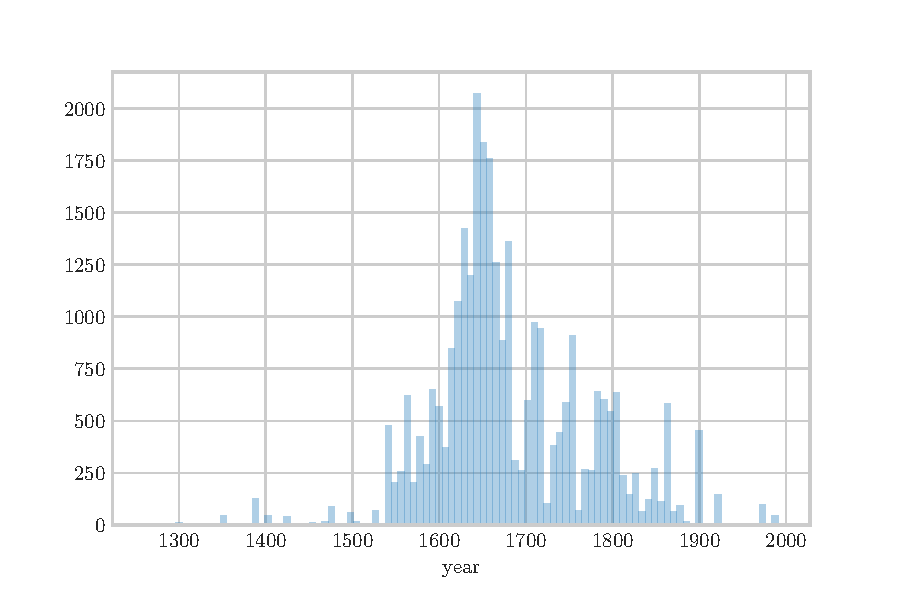
\includegraphics[scale=0.9]{histyeartotal}
	\caption{Distribution of the songs by year (1260-1991) in the sample (\textit{n} = 29,590)}
	\label{fig:DistSongs}
\end{figure}

Since the genre of the song was also tagged in the XML-file, I am able to see how the songs are distributed over the various categories (see Table~\ref{table:SongsCat}). A major part of the songs belong to the genre \enquote{religion}, followed at a distance by \enquote{love and sex},  \enquote{seasons and annual events}, \enquote{formal genres} and \enquote{amusement}. One might ask why a study on topics in song lyrics is useful, since we already have these data on categories, but you can argue with that. This categorical division not only seems a bit arbitrary (when does a song belong to \enquote{work}? What is a \enquote{formal genre}? What are the differences between songs on \enquote{seasons and annual events} and songs on \enquote{occasions}?), there are also more than 9000 songs that have not been assigned to a category. These data thus does not give reliable information about the distribution of songs over different genres. Besides that, the wide-ranging categories don't reveal how subdivisions within a category are distributed. Are all religious songs on the same aspects of religion? Does \enquote{love and sex} mean that some songs are on love, and others on sex? Which words are used to describe the one or the other? In summary, there is an important difference between a genre and a topic, since a genre can comprise many different topics. Topic modeling can give answers to the above questions.

\begin{table}
	\centering
	\begin{tabular}{lr}
		\toprule
		category                  & id        \\
		\midrule
		None                  &  7017 \\
		religion                     &   6914 \\
		love and sex              &   3261 \\
		seasons and annual events &   1033 \\
		formal genres                  &   818 \\
		amusement             &   722 \\
		emotions                &    694 \\
		narratives      &    479 \\
		cycle of life                &    473 \\
		politics and history             &    300 \\
		groups                    &    187 \\
		children                  &    148 \\
		occasions                 &    100 \\
		theatre                   &     90 \\
		work                      &     59 \\
		miscellaneous             &      2 \\
		\bottomrule
	\end{tabular}
	\caption{Number of songs per category (\textit{n} = 22,297)}
	\label{table:SongsCat}
\end{table}

\begin{figure}[hbt!]
	\centering
	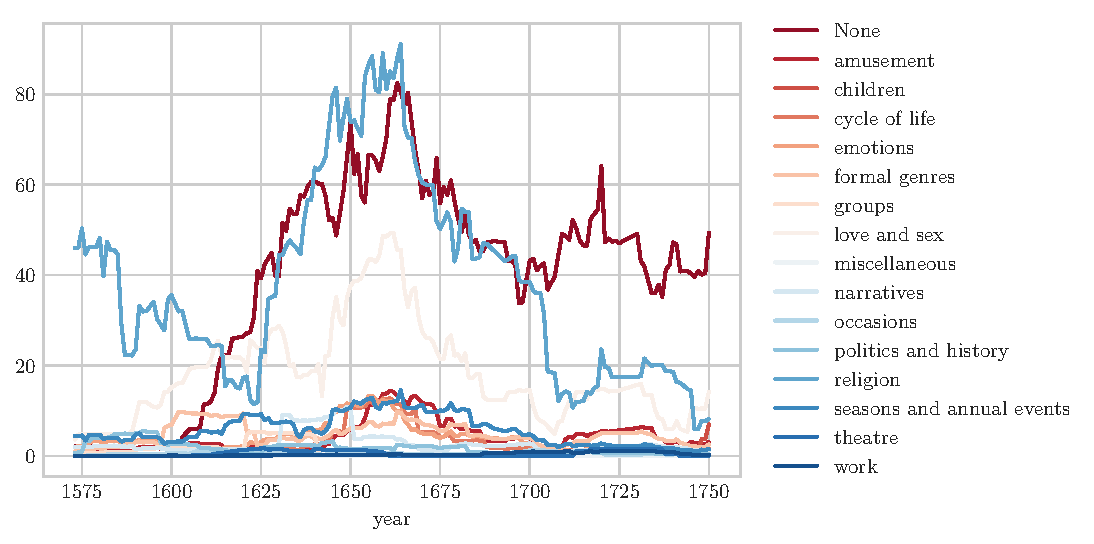
\includegraphics[scale=0.75]{categoriesdist2}
	\caption{Distribution of the categories (\textit{n} = 22,297)}
	\label{fig:CatDist}
\end{figure}

However, the corpus in its current state is not complete yet. It does not include the reprints and appearances of these songs in other songbooks. Since I want to examine which song topics were more prevalent than others, it is necessary to include these data as well. Although the number of lyrics will remain the same, the distribution of the songs can change. Imagine for example that songs on politics and history, which are not very prominent in the corpus based on the data in Table ~\ref{table:SongsCat}, are reprinted so often that their number will increase massively, while songs on love are hardly reprinted. This might influence the distribution of topics. The DSD contains the needed data for this extension of the corpus, but in order to extract them, it is import to understand the terminology that is used in the database. Each first print of a song has a \textit{recordid}, which is the \texttt{id} that is mentioned in the XML-file of a song. A reprint of a song does not contain a \textit{recordid}, but a \textit{herdrukid} instead. Furthermore, each unique song has an \textit{incnormid}. This means that a couple of songs with different \textit{recordid}'s and \textit{herdrukid}'s share the same \textit{incnormid}. I added songs to my corpus with the same \textit{incnormid} and/or \textit{recordid} as the ones already in the corpus, resulting in a corpus of 43,772 songs. Their distribution over time is visualized in Figure~\ref{fig:DistSongsSample}. The next step is to make the lyrics of these songs ready for building topics from it.

\begin{figure}[hbt!]
	\centering
	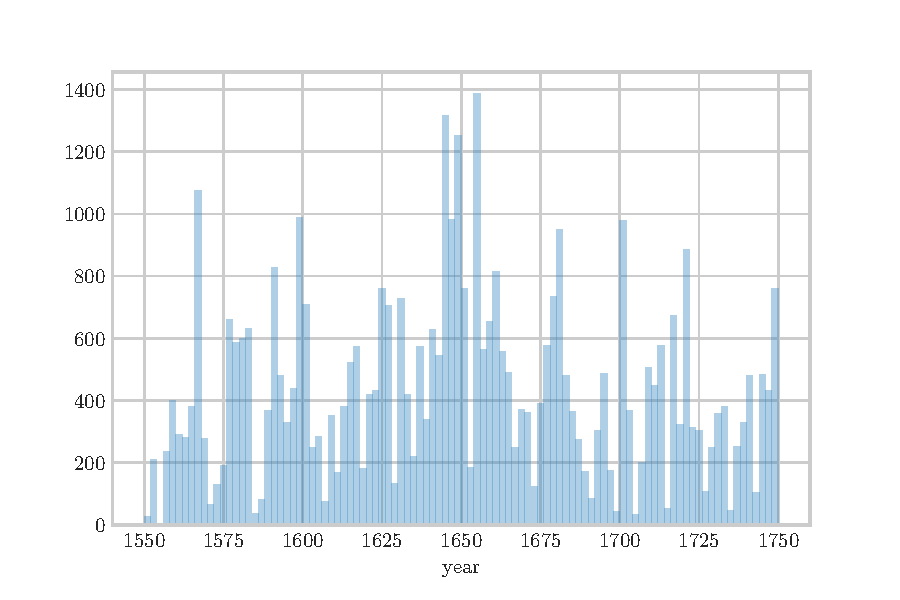
\includegraphics[scale=0.9]{histyearall}
	\caption{Distribution of the songs by year (1550-1750) in the sample (\textit{n} = 43,772)}
	\label{fig:DistSongsSample}
\end{figure}

	\chapter{Spelling normalization}
In the sixteenth and seventeenth century, Dutch authors and printers didn't highly value the consistency of word spellings. This resulted in many different spelling variants of the same word coexisting. Because a topic modeling method only looks at the position of words and how they are distributed through the corpus, it sees different spellings of the same word as different words. For instance, \enquote{Jezus}, \enquote{Jesu} and \enquote{Iesus} are regarded as different words, as well as \enquote{bloed} and \enquote{bloet}. It is easy to understand that this biases the results of the topic modeling process. Therefore normalization of spelling is a crucial step that needs to be taken. Regarding the English language, quite some tools are available for converting historical texts to a standard spelling. For the Dutch language, options are limited, especially methods that are straightforward method and do not cost too much time. The tools that are available, come with both advantages and disadvantages. I have chosen to use two different methods to normalize the spelling of my corpus. After normalization with these two methods, I will perform topic modeling on the two different normalized versions of my corpus, as well on the unnormalized version of my corpus, e.g. the original texts. Hopefully the results of topic modeling will give more insight which version of the corpus is the most productive to work with. Below I discuss the two tools that I will use for spelling normalization. To illustrate the performance of both tools, I will show the normalized spelling versions of one particular song lyric\footnote{\texttt{id} = 186989.} later on. Here I show the original version of this song:

\begin{quote}
	Daar de gulde zon en maan\\
	En de mindre hemelvieren,\\
	Die het stargewelf vercieren,\\
	Gods geboden gadeslaan:\\
	Daar de felle noordewinden\\
	In het bruissend element\\
	Op die stem zig laten binden:\\
	Wie roept dat hy God niet kent?\\
	
	'T aards gezinde en dwaze rot\\
	Op het vroom geslagt verbolgen\\
	En geneigt zijn lust te volgen,\\
	Durft zig uiten, daar 's geen God.\\
	Welkers oordeel sta te vreezen\\
	Als het lighaam zinkt in 't graf.\\
	Want de ziel verliest haar wezen,\\
	Als wy leggen 't leven af.\\
	
	Aartsverraders schrikt, ziet toe\\
	Gods gedult, en hand te tergen.\\
	Voor zijn oog is geen verbergen.\\
	Vreest, vreest 's Hemels strenge roe!\\
	Eenmaal zal de dag genaken.\\
	(Is zijn wrake traag in 't gaan)\\
	Die u zal te schande maken,\\
	En door blixemvuur verslaan.
\end{quote}

\section{INL}
The first method I have used to modernize spelling is a tool built by Marijn Schraagen and Martijn van der Klis. The modernization is performed by querying all words in the corpus using the INT Lexicon Service\footnote{http://sk.taalbanknederlands.inl.nl/LexiconService/.} and replacing the words with the lemma resulting from the query. An important note is that the tool cannot be trained: the first result of the query in the Lexicon Service is always chosen as output, and this can not be manipulated. This means that it's hard to correct the mistakes that are made by the tool. In addition, all verbal words are normalized to the infinitive, which means that the difference between past and present forms disappears. After normalization with INL, the song mentioned above looks like this:

\begin{quote}
	Daar de gild zon en maan\\
	En de minder hemelvieren\\
	Die het stergewelf versieren\\
	Gods geboden gadeslaan :\\
	Daar de fel noordewinden\\
	In het bruissend element\\
	Op die stem zek laten binden :\\
	Wie roepen dat hei God niet ken ?\\
	
	'T aards gezinde en dwaas rot\\
	Op het vroom geslacht verbolgen\\
	En neigen zijn lust te volgen\\
	Durft zek uiten daar de geen God\\
	Welkers oordeel staan te vrees\\
	Als het lichaam zinken in 't graf\\
	Want de ziel verliezen haar wezen\\
	Als wi leggen 't leven af\\
	
	Aartsverraders schrikken zeer toe\\
	Gods geduld en hand te tergen\\
	Voor zijn oog is geen verbergen\\
	Vreest vrezen de Hemels streng roede !\\
	Eenmaal zullen de dag genaken\\
	( Is zijn wraak traag in 't gaan )\\
	Die u zullen te schande maken\\
	En door blixemvuur verslaan
\end{quote}

\noindent Although this song's lyrics were already quite easy to read, the tool has changed some words to a modern form (\enquote{vercieren} becomes \enquote{versieren}, \enquote{geslagt} becomes \enquote{geslacht}). It also made several mistakes. In the first line, \enquote{gulde} is normalized to \enquote{gild}, but that should have been \enquote{gulden} or \enquote{gouden}. The word \enquote{zig} is normalized to \enquote{zek}, which is not even a word. Other mistakes include the changing of \enquote{hy} into \enquote{hei}, and \enquote{'s} into \enquote{de}. Furthermore, this example shows that verbal forms are changed into the infinitive: \enquote{verliest} becomes \enquote{verliezen}, \enquote{zal} becomes \enquote{zullen}. Strange is that \enquote{Vreest, vreest} is normalized to \enquote{Vreest vrezen} instead of \enquote{vrezen vrezen}. That might be caused by the capital \enquote{V}. Figure~\ref{fig:NormWordtypes} shows the reduction of unique words after normalizing the original corpus with the INL tool -- this number has only decreased with 1\% (1,832 unique words).

\begin{figure}[hbt!]
	\centering
	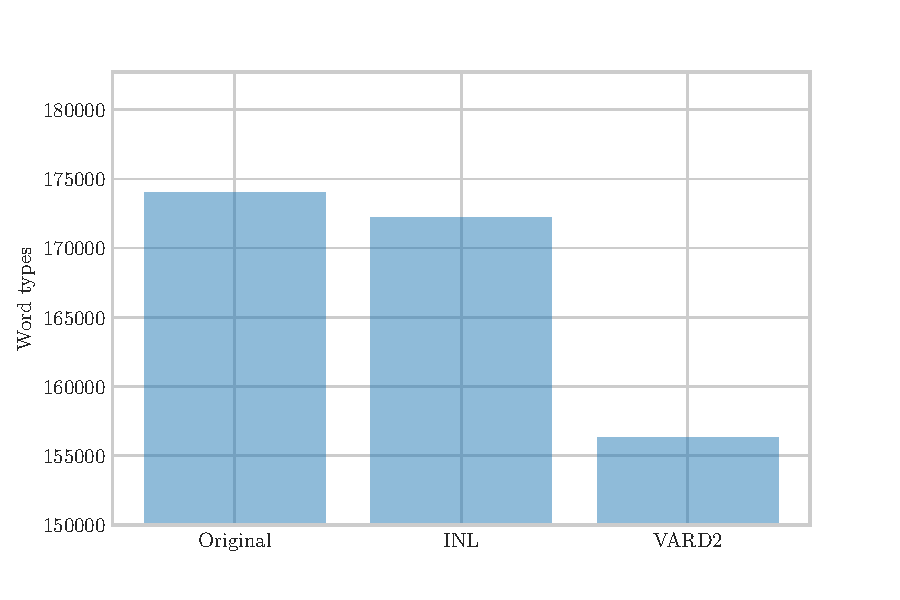
\includegraphics[scale=0.9]{Effect_normalization}
	\caption{Effect of normalization on number of word types}
	\label{fig:NormWordtypes}
\end{figure}

\section{VARD2}
A more reliable tool seems the semi-automatic tool VARiant Detector (VARD), in 2005 introduced by Alistair Baron and Paul Rayson. The tool uses two lists (a normalized word list and a variant list) to suggest or replace variant words with their normalized counterparts. VARD \textit{(i)} reads a given text, \textit{(ii)} distinguishes variants within the text, \textit{(iii)} chooses the most appropriate normalized form for each variant found and \textit{(iv)} matches the variant with the normalized form.\autocite{archer_guidelines_2015} This first version of the tool used a manually created list of variants to modern equivalent mappings in order to search for and replace any spelling variants found within a text. However, it was impossible to include all possible spelling variants in a pre-defined list and therefore the tool was not of use when dealing with spelling variations in other languages than Early Modern English. Therefore, a more recent version of the tool, VARD2, was developed with a more flexible approach which allows the tool to deal with a much larger variety of spelling variants. The normalization suggestions are given, based on a combination of four different methods: \textit{(i)} known variant replacements, \textit{(ii)} character edit distance, \textit{(iii)} letter rules and \textit{(iv)} phonetic distance. \autocite{baron_vard_nodate}

In this thesis I use a setup of VARD2 that is trained to perform spelling normalization on Dutch historical texts. It was built by Ivan Kisjes and Tessa Wijckmans, as a result of a collaboration between the CREATE-project of the University of Amsterdam and the Dutch digital research platform \textit{Nederlab}. Kisjes and Wijckmans presented the setup in a paper titled \enquote{Adapting a Spelling Normalization Tool Designed for English to 17th Century Dutch} during the Digital Humanities Conference in Mexico City in 2018.\autocite{kisjes_adapting_2018} Kisjes and Wijckmans created a Dutch configuration of VARD2, using the modifiable parts of VARD2: the letter rules, the variant list and the normalized word list. As a training set they used the 1657 edition of the Dutch translation of the Bible. There were two important reasons for this choice: first, there was a modern translation of the bible available that stuck rather closely to the original word order, and second, since there was another edition of the bible printed in 1637 available, it would be possible to easily find more spelling variants for the words they had manually respelled or checked in the 1637 edition.

In the VARD2 tool it is possible to manually process a single text as well as to process a big corpus of texts. Words of texts are placed either manually or automatically into one of the following three categories: \textit{variants}, \textit{non variants} and \textit{normalized words}. VARD2 adds words to the variant category when they are not found in its real word list. Moreover, the user can add words to this category manually as well. The variant category contains all words which the system considers necessary to normalize. The normalized category contains all words which have been normalized by the user or through automatic processing. The non variants category contains all words which are in the modern lexicon. Besides the option to processing a single text, VARD2 also offers the opportunity to process a batch of texts. In that case, the manual normalization option is not available, only the automatic normalization option.

\begin{table}[]
	\centering
	\begin{tabular}{lllll}
		\toprule
		Threshold (\%) & Variants & Variants (\%) & Normalized & Normalized (\%) \\ \midrule
		30             & 122      & 12.18         & 345        & 34.43           \\
		40             & 122      & 12.18         & 345        & 34.43           \\
		50             & 123      & 12.28         & 344        & 34.33           \\
		60             & 144      & 14.37         & 323        & 32.24           \\
		70             & 152      & 15.17         & 315        & 31.44           \\
		80             & 219      & 21.86         & 248        & 24.75           \\
		90             & 263      & 26.25         & 204        & 20.36   \\  
		\bottomrule     
	\end{tabular}
	\caption{VARD2-results at different thresholds (\texttt{id} = 11218, number of tokens = 467, number of non variants = 535)}
	\label{table:VardTresholds}
\end{table}

VARD2 will generally find numerous potential normalizations for a given variant. Each of these suggestions is given a confidence score. In the case of automatic processing, the suggested normalization with the highest confidence score is used to replace each variant. However, if the system's normalization methods \enquote{struggle} with a particular variant, the highest confidence score may be relatively low -- in these cases a threshold is required, which is the minimum confidence score needed for a normalization to take place. If the threshold is not met by the top normalization suggestion, the word is left as a variant. To get a feel for a suitable threshold for my corpus, I used a single text of my corpus and checked which number of words were normalized at different thresholds. A higher threshold will increase precision (less variants will be normalized) but reduce recall. In Table~\ref{table:VardTresholds} the results are shown for different thresholds when processing one particular song (id = 11218).\footnote{I chose this song because it has a high number of word types.} These results show that there is hardly any difference between a threshold of 30\% and 50\%. The higher the threshold, the less variants are normalized. Since I observed that the tool didn't perform any wrong normalizations, I decided to set the threshold rather low, at 50\%. The above mentioned song contains the following lyrics after normalization with VARD2:

\begin{quote}
	Daar de gulde zon en maan\\
	En de mindre hemelvieren,\\
	Die het stargewelf versieren,\\
	Gods geboden gadeslaan:\\
	Daar de felle noordewinden\\
	In het bruissend element\\
	Op die stem zig laten binden:\\
	Wie roept dat hij God niet kent?\\
	
	Het aards gezinde en dwaze rot\\
	Op het vroom geslagt verbolgen\\
	En geneigd zijn lust te volgen,\\
	Durft zig uiten, daar des geen God.\\
	Welkers oordeel sta te vrezen\\
	Als het lighaam zinkt in het graf.\\
	Want de ziel verliest haar wezen,\\
	Als wij leggen het leven af.\\
	
	Aartsverraders schrikt, ziet toe\\
	Gods geduld, en hand te tergen.\\
	Voor zijn oog is geen verbergen.\\
	Vreest, vreest des Hemels strenge roe!\\
	Eenmaal zal de dag genaken.\\
	(Is zijn wrake traag in het gaan)\\
	Die u zal te schande maken,\\
	En door blixemvuur verslaan.\\
\end{quote}

\noindent Most of the wrong normalizations that the INL tool performed, are not made by the VARD2 tool: \enquote{gulde} and \enquote{zig} stay the same, as well as the verbal forms. The words \enquote{vercieren} and \enquote{hy} are correctly changed into \enquote{versieren} and \enquote{hij}. Besides that, the VARD2-tool replaces \enquote{'t} with \enquote{het}. Although in this example less words are substituted with the VARD2- tool, Figure~\ref{fig:NormWordtypes} shows that, after normalization with VARD2, the number of unique words in the corpus was reduced with 17,692, which is 10\% of the total number of unique words. This suggests that the VARD2 tool obtains better results than the INL tool, but the topic modeling results should give more insight in this case.
	\chapter{Topic models and turnovers}

\section{LDA}
To perform topic modeling, I use the Python package \texttt{gensim}, which contains \texttt{models.wrappers.ldamallet}, a wrapper for Latent Dirichlet Allocation (LDA) from MALLET, a Java topic modeling toolkit. The module uses an optimized version of collapsed Gibbs sampling from MALLET. MALLET (Machine Learning for Language Toolkit) is a package for several machine learning applications to text, such as statistical natural language processing, document classification and clustering. LDA is the most commonly used topic modeling method. \enquote{Latent} refers to the concept of latent distributions in the model, and \enquote{Dirichlet} is the name of the most common used prior distribution, named after the German mathematician Johann Dirichlet (1805-1859). It consists of a nested multilevel structure, in which the following three levels need to be distinguished:\autocites[995]{blei_latent_nodate}{blei_probabilistic_2010}
\begin{itemize}
	\item A \textit{word} is an item from a vocabulary indexed by \{$1,...,V$\}. Words are represented using unit-basis vectors that have a single component equal to one and all other components equal to zero. Thus, using superscripts to denote components, the \textit{v}th word in the vocabulary is represented by a \textit{V}-vector \textit{w} such that $w^{v} = 1$ and $w^{u} = 0$ for $u \neq v$.
	\item A \textit{document} is a sequence of \textit{N} words denoted by \textit{d} $= (w_{1},w_{2},...,w_{N})$, where $w_{n}$ is the $n$th word in the sequence.
	\item A \textit{corpus} is a collection of \textit{M} documents denoted by $D = \{\textit{d}_{1},\textit{d}_{2},...,\textit{d}_{M}\}$.
\end{itemize}
Furthermore, a \textit{topic} $\phi$ is a distribution over a fixed vocabulary of \textit{V} words. The words \textit{w} of each document \textit{d} will be associated with a mixture of \textit{K} distributions. \textit{K} stands for the number of topics you want the model to create, and is the only parameter that has to be fixed in advance.\footnote{There are also topic models which infer \textit{K} from data.} The probability of an individual word is the sum over all topics of the word's probability in a topic times the probability of a topic in the current document. The probability of a document is written as follows: \autocite[277]{karsdorp_humanities_2019}

\begin{equation}
p\left(\vec{w}_{d}\right)=\prod_{i}^{n_{d}} p\left(w_{d, i}\right)=\prod_{i}^{n_{d}} \sum_{k}^{K} \theta_{d, k} \operatorname{Categorical}\left(w_{d, i} | \vec{\phi}_{k}\right)
\end{equation}

\noindent where $\operatorname{Categorical}\left(x | \vec{\phi}_{k}\right)=\prod_{v}^{V} \phi_{k, v}^{x(v)}$. However, this is just the beginning. The equation above is a model of the words associated with a single document, but I need to model all \textit{N} words in the \textit{M} documents in my corpus \textit{D}. In this way I will be able to model the topological homogeneity which exists across documents. Furthermore, I need to allow each document to have distinct topic weights, since some documents will feature certain latent distributions more prominently than others. The following steps need to be taken:

\begin{enumerate}
	\item For each topic \textit{k}, sample a probability distribution $\phi_{k}$ from Dirichlet($\eta$).
	\item For each document \textit{d}:
	\begin{enumerate}
		\item Sample a document-specific set of topic proportions, $\theta_{d}$, from a Dirichlet distribution with parameter $\alpha$.
		\item For each word $w_{d,i}$ in document \textit{d}:
		\begin{enumerate}
		\item Sample a word-specific latent mixture component, $z_{d,i}$ from the document-specific topic proportions $\theta_{d}$.
		\item Sample a word from the latent distribution, $w_{d,i} \sim \operatorname{Categorical}(\eta_{z_{d,i}})$.
		\end{enumerate}
	\end{enumerate}
\end{enumerate}

\noindent The probability of the entire corpus is then written as follows:

\begin{equation}
\begin{aligned} p\left(w_{1 : D} | \theta_{1 : D}, \phi_{1 : K}\right)=\prod_{d=1}^{D} p\left(w_{d}\right) &=\prod_{d=1}^{D} \prod_{i}^{n_{d}} p\left(w_{d, i} | \theta_{d}, \phi_{1 : k}\right) \\ &=\prod_{i}^{n_{d}} \sum_{k}^{K} \theta_{d, k} \operatorname{Categorical}\left(w_{d} | \phi_{k}\right) \end{aligned}
\end{equation}
\noindent The earlier mentioned three levels in a LDA representation (word, document, corpus) have their own variables. The parameters $\alpha$ and $\phi$ are corpus-level parameters, the variables $\theta_{d}$ are document-level variables and the variables $z_{d,i}$ and $w_{d,i}$ are word-level variables. The three-level-structure of LDA ensures that one document can be associated with multiple topics, not with just one. \autocite[997]{blei_latent_nodate} With LDA, a document collection is analyzed by examining the posterior distribution of the latent variables. Posterior inference means that the generative process is reversed several times. Conditioned on a corpus, the goal of posterior inference is to find the posterior distribution over alternative topical structures that generated its document.\autocite{blei_probabilistic_2010} Posterior modes of the topics $\phi_{1:K}$ identify corpus-wide patterns of words; posterior modes of the topic proportions $\theta_{d}$ identify how the $d$th document expresses those patterns; posterior modes of the topic assignments $z_{d,i}$ identify which topics the $n$th word of the $d$th document is associated with.\autocite{blei_probabilistic_2010}

\section{Calculating turnover series}
For the calculation of turnover profiles in the context of this study, I draw inspiration from a chapter on turnover in \textit{Humanities Data Analysis} (to be published) from Folgert Karsdorp, Mike Kestemont and Alan Riddel. They state that turnover \enquote{can be defined as the number of new names that enter a popularity-ranked list at position \textit{n} at a particular moment in time \textit{t}.}\autocite[126]{karsdorp_humanities_2019} To compute a turnover series, they distinguish the next three steps:

\begin{quote}
	first, we can calculate an annual popularity index, which contains all unique names of a particular year ranked according to their frequency of use in descending order. Subsequently, the popularity indexes can be put in chronological order, allowing us to compare the indexes for each year to the previous year. For each position in the ranked lists, we count the number of \enquote{shifts} in the ranking that have taken place between two consecutive years. This \enquote{number of shifts} is called the turnover. Computing the turnover for all time steps in our collections yields a turnover series.\autocite[126]{karsdorp_humanities_2019}
\end{quote}

\noindent This method can be applied to the subject of this research, although some preliminary steps need to be taken. The following procedure needs to be carried out:

\begin{enumerate}
	\item For each song in the corpus:
	\begin{enumerate}
		\item Calculate the topic distribution using MALLET.
		\item Connect the year of print of the song to this topic distribution.
	\end{enumerate}
	\item Calculate an annual popularity index, containing all song topics, ranked according to their frequency of appearance in descending order.
	\item Put the annual popularity indexes in chronological order, in order to compare the indexes for each year to the previous year.
	\item For each position in the ranked lists, count the number of \enquote{shifts} in the ranking that have taken place between two consecutive years. This \enquote{number of shifts} is called the turnover.
	\item Compute the turnover for all time steps, which yields a turnover series.
\end{enumerate}

\noindent In Chapter 8, I will carry out this procedure and see if a certain transmission bias can be derived from the shape of the turnover plot.
\part{Analysis and results}
	\chapter{Dominant topics}
With the three versions of my corpus (original, INL-normalized and VARD2-normalized), I continue my analysis. To build topic models with \texttt{gensim}, I have to take a few preliminary steps. In this chapter I will therefore first explain how a corpus needs to be prepared in order to perform topic modeling and how I have chosen the optimal settings. Afterwards, I will build the final topic models and discuss the results.

\section{Preparation of data and choosing settings}
At first, a corpus needs to be tokenized. This means that each text will be converted to a list with separate words, and that punctuation will be removed. Besides that, it is useful to filter \enquote{stop words} from the corpus. Stop words are the very common words in a corpus, which are in this case mostly function words such as \textit{ik} (personal pronoun), \textit{de} (preposition) and \textit{en} (conjunction). Content words, which have a more specific meaning, are often less frequent than function words. I created a list with the 150 most frequent words, using the Python package \texttt{nltk.FreqDist} after tokenization with \texttt{nltk.tokenize.word\_tokenize(language="dutch")}. I did this once for each version of my corpus. I checked each list manually and removed the function words from it (see Table~\ref{table:RemovedWords}). The three stop lists can be found in the appendix. I used the code below:\footnote{In this paragraph I show the code and results from the preprocess of the VARD2-normalized corpus. For building topic models from the other corpora, I used the same settings.}

\begin{lstlisting}
	import glob
	import nltk
	from utils import is_punct
	
	TOKENIZER = nltk.tokenize.word_tokenize
	CORPUS_PATH = "Corpus/VARDnormalized/varded50/*.txt"
	STOP_WORDS_PATH = "stoplists/stoplist_VARD2.txt"
	STOP_WORDS = [s.lower() for s in open(STOP_WORDS_PATH, "r", encoding="utf-8").read().splitlines()]
	
	remove_stopwords = lambda x: [word.lower() for word in x if word.lower() not in STOP_WORDS and not is_punct(word) and len(word) > 1]
	
	texts = glob.glob(CORPUS_PATH, recursive=False)
	tokenized_texts = [TOKENIZER(open(text, "r", encoding="utf-8").read(), language="dutch") for text in texts]
	tokenized_texts = [remove_stopwords(text) for text in tokenized_texts]
\end{lstlisting}

\noindent I added \texttt{len(word) > 1} to the function \texttt{remove\_stopwords} to make sure that no punctuation was left that for some reason was not included in the function \texttt{is\_punct}. After tokenization and punctuation removal, the song that was also discussed in the previous chapter, looked like this:

\begin{lstlisting}
["gulde", "zon", "maan", "mindre", "hemelvieren", "stargewelf", "versieren", "gods", "geboden", "gadeslaan", "felle", "noordewinden", "bruissend", "element", "stem", "zig", "laten", "binden", "roept", "god", "kent", "aards", "gezinde", "dwaze", "rot", "vroom", "geslagt", "verbolgen", "geneigd", "lust", "volgen", "durft", "zig", "uiten", "god", "welkers", "oordeel", "sta", "vrezen", "lighaam", "zinkt", "graf", "ziel", "verliest", "leggen", "leven", "af", "aartsverraders", "schrikt", "gods", "geduld", "hand", "tergen", "oog", "verbergen", "vreest", "vreest", "hemels", "strenge", "roe", "eenmaal", "genaken", "wrake", "traag", "schande", "maken","blixemvuur", "verslaan"]
\end{lstlisting}

\begin{table}[]
	\centering
	\begin{tabular}{ll}
		\toprule
		Corpus & removed words \\
		\midrule
		Original & \makecell{godt, heer, god, hert, leven, liefde, ziel, gods, heere, lief,\\min, heeren, godts, recht, mensch, menschen, lust}                                  \\
		INL      & \makecell{leven, heer, godt, hert, ziel, vreugde, hart, liefde, mens, tijd,\\gods, heere, kwaad, lief, zondaar, dag, dood, grond, eeuwig,\\kracht, wereld, hand} \\
		VARD2    & \makecell{god, gods, leven, hert, ziel, liefde, tijd, vreugd, here, geest,\\woord, lief, min, kwaad, zonden, heren, lof, hand, wereld,\\mens, mensen, recht} \\
		\bottomrule
	\end{tabular}
	\caption{Removed words from stop lists}
	\label{table:RemovedWords}
\end{table}

\noindent The two main inputs to a LDA topic model are \texttt{dictionary} and \texttt{corpus}. A dictionary is a commonly used \texttt{python} data type, containing \textit{key: value} pairs. Keys can be any immutable type, with the requirement that keys are unique within one dictionary. The keys of this dictionary are all unique tokens that exist in \texttt{tokenized\_texts}. The corresponding values are the number of times the words appear in \texttt{tokenized\_texts}. \texttt{gensim} creates a unique id for each word in a text. With \texttt{corpus}, a corpus is produced from \texttt{dictionary}, resulting in a mapping of [word\_id, word\_frequency].

\texttt{gensim} gives the opportunity to remove terms from the dictionary that appear too frequently or too infrequently in the corpus. This can be done with the functions \texttt{no\_below} and \texttt{no\_above}. The input for \texttt{no\_above} needs to be a number between 0 and 1: if \texttt{no\_above = 0.80}, terms that appear in more than 80\% of the documents are ignored. The input for \texttt{no\_below} needs to be an absolute number, corresponding with an actual number of documents: if \texttt{no\_below = 20}, terms that appear in less than 20 documents are ignored. The \texttt{no\_above} function can be seen as a tool to remove \enquote{corpus-specific stop words}. Since I already created a list with corpus-specific words, using the \texttt{no\_above} function is unnecessary. I therefore use \texttt{no\_above = 1}, implying that only tokens are removed that appear in more than 100\% of the documents, which, in fact, are zero tokens. Deciding what the right setting for \texttt{no\_below} is, is a bit of trial and error. I built three dictionaries (with \texttt{no\_below = 2}, \texttt{no\_below = 5} and \texttt{no\_below = 10}), using the following code:

\begin{lstlisting}
import gensim
from gensim import corpora
from gensim.corpora import Dictionary

NO_BELOW = 2 #and 5 and 10. minimum document frequency (absolute)
NO_ABOVE = 1 #maximum document frequency (fraction)

dictionary = Dictionary(tokenized_texts)
dictionary.filter_extremes(no_below=NO_BELOW, no_above=NO_ABOVE)
corpus = [dictionary.doc2bow(text) for text in tokenized_texts]
\end{lstlisting}

\noindent Table~\ref{table:DictSizesDifferentNB} contains the dictionary sizes at different settings for \texttt{no\_below}. It turns out that a rather big amount of tokens are discarded in all cases. At \texttt{no\_below = 2}, all tokens are removed that appear in only one text. This number of tokens is already quite high: 117,045. The number of discarded tokens only grows extensively when increasing \texttt{no\_below}. At \texttt{no\_below = 10}, only 19,912 tokens remain. This seems a really small number, but when we keep in mind that only those words are removed that appear in less than ten songs (out of a total number of 22,297 songs), this cut-off seems very reasonable.

\begin{table}[]
	\centering
	\begin{tabular}{llll}
		\toprule
		no\_below & 10 & 5 & 2 \\
		\midrule
		Discarded tokens & 174,247                & 160,705                & 117,045                \\
		Kept tokens      & 19,912                 & 33,454                 & 77,114          \\
		\bottomrule      
	\end{tabular}
	\caption{Dictionary sizes at different no\_below's}
	\label{table:DictSizesDifferentNB}
\end{table}

To make more sense of these numbers, I built a topic model for each setting of \texttt{no\_below} and compared the coherence score of each topic model.  The topic coherence provides a measure to judge how good a given topic model is. The output is a number between 0 and 1. The higher this number, the better the topic model. For the time being, I let the model create 50 topics. To build the topic model and to compute the coherence score, I used the following code:

\begin{lstlisting}
from gensim.models import CoherenceModel
from gensim.models.wrappers import LdaMallet

N_TOPICS = 50
ITERATIONS = 2000
OPTIMIZE_INTERVAL = 20
EVAL_EVERY = 3 #for regular LDA
N_WORKERS = 3 #number of CPU'S for multiprocessing

lda = LdaMallet("/Users/alielassche/applications/mallet/bin/mallet", corpus=corpus, id2word=dictionary, num_topics=N_TOPICS, iterations=ITERATIONS, workers=N_WORKERS, optimize_interval=OPTIMIZE_INTERVAL)

# Compute Coherence score
coherence_model_ldamallet = CoherenceModel(model=lda, texts=tokenized_texts, dictionary=dictionary, coherence="c_v")
coherence_ldamallet = coherence_model_ldamallet.get_coherence()
\end{lstlisting}

\noindent The results are stored in Table~\ref{table:CSDiffNB}. It turns out that the topic model made with \texttt{no\_below = 2} has the highest coherence score. Therefore I continue with that parameter setting.

\begin{table}[]
	\centering
	\begin{tabular}{ll}
		\toprule
		no\_below & Coherence score  \\
		\midrule
		2 & 0.50571         \\
		5 & 0.49573     \\
		10 & 0.49014 \\
		\bottomrule      
	\end{tabular}
	\caption{Coherence score at different no\_below's}
	\label{table:CSDiffNB}
\end{table}

The next step is to choose the number of topics. Since this parameter can highly influence the results, I use the coherence score here as well. With the code below, I calculate the coherence score for 10 topic models with different values for \texttt{num\_topics}, in the range 10:100.

\begin{lstlisting}
def compute_coherence_values(dictionary, corpus, texts, limit, start=2, step=3):

	coherence_values = []
	model_list = []
	for num_topics in range(start, limit, step):
	model = gensim.models.wrappers.LdaMallet
	("/Users/alielassche/applications/mallet/bin/mallet", corpus=corpus, num_topics=num_topics, id2word=dictionary, iterations=ITERATIONS,  
	workers=N_WORKERS, optimize_interval=OPTIMIZE_INTERVAL)
	model_list.append(model)
	coherencemodel = CoherenceModel(model=model, texts=tokenized_texts, dictionary=dictionary, coherence="c_v")
	coherence_values.append(coherencemodel.get_coherence())
	
	return model_list, coherence_values
	
	# model_list: List of LDA topic models
	# coherence_values: Coherence values corresponding to the LDA model with respective number of topics
	
model_list, coherence_values = compute_coherence_values(dictionary=dictionary, corpus=corpus, texts=tokenized_texts, start=10, limit=110, step=10)
\end{lstlisting}

\begin{figure}[hbt!]
	\centering
	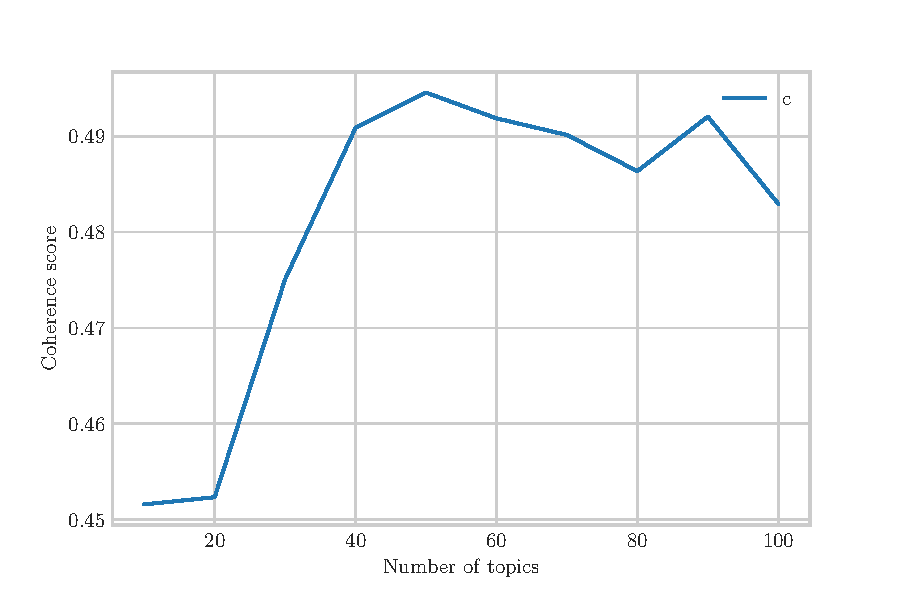
\includegraphics[scale=0.9]{coherence_values_2_10_100}
	\caption{Choosing an optimal number of topics with coherence scores}
	\label{fig:ChoosingTopicsWithCS}
\end{figure}

\noindent The results are plotted in Figure~\ref{fig:ChoosingTopicsWithCS}. The highest coherence score is obtained at \texttt{num\_topics = 50}. I therefore decided to build the final topic models using this setting. 

\section{Building the final topic models}
I built the final topic models for the three versions of my corpus with the following code:

\begin{lstlisting}
NO_BELOW = 2 #minimum document frequency
NO_ABOVE = 1 #maximum document frequency

N_TOPICS = 50
ITERATIONS = 2000
OPTIMIZE_INTERVAL = 20
EVAL_EVERY = 3 # for regular LDA 
N_WORKERS = 3 # number of CPU'S for multiprocessing

lda = LdaMallet("/Users/alielassche/applications/mallet/bin/mallet", 
corpus=corpus, id2word=dictionary, num_topics=N_TOPICS, iterations=ITERATIONS, workers=N_WORKERS, optimize_interval=OPTIMIZE_INTERVAL)
\end{lstlisting}

\noindent The most basic and important output of the function \texttt{LdaMallet} is two dataframes: one with the keys of a topic model, the other one with the composition. The dataframe \texttt{keys} contains 50 rows, for each topic one, and 2 columns: one for the topic number, the other one for the words that form a specific topic. The dataframe \texttt{composition} contains as many rows as there are texts in the corpus: in this case 22,297. The columns are numbered from 0 to 49, corresponding with the numbers of the topics from \texttt{keys}. The cells from each row contain the composition of the 50 topics in that text. The higher a value, the more dominant a topic is in a text. Other characteristics of the model, the topics or the texts can be obtained, but I will discuss that in more detail below, where I analyze the results of \texttt{LdaMallet} by the version of the corpus.

\subsection{Original corpus}
The dictionary that was built from the original corpus, contained at first 218,027 unique tokens, but after discarding 127,936 tokens (the number of tokens with a value of \texttt{1} in the dictionary, a result of the setting \texttt{no\_below = 2}), 90,091 tokens remained. I let the tool build 50 topics from this corpus and dictionary. The coherence score of the model was 0.5097. All topics with their corresponding words can be find in the appendix, but the most self-explanatory topics I show in some word clouds in the Figures~\ref{fig:topic3Original} to~\ref{fig:topic49Original}. I have to assign a word to each topic, with which the subject of the topic can be described. I assigned the subject \textit{love and sadness} to topic 3, which is pictured in Figure~\ref{fig:topic3Original}, because of the presence of positive words such as \enquote{lief}, \enquote{lieve}, \enquote{min} and \enquote{schoone} on the one hand and negative words as \enquote{smert}, \enquote{tranen}, \enquote{verdriet} and \enquote{pijn} on the other hand. This topic differs from another love-topic, topic 49 (Figure~\ref{fig:topic49Original}), in such way that almost all words in this topic are positive words: \enquote{hert}, \enquote{zoet}, \enquote{min}, \enquote{vreugd} and \enquote{lief}. I assign the subject \textit{love \& happiness} to this topic.

\begin{figure}
	\begin{minipage}[c]{0.48\linewidth}
		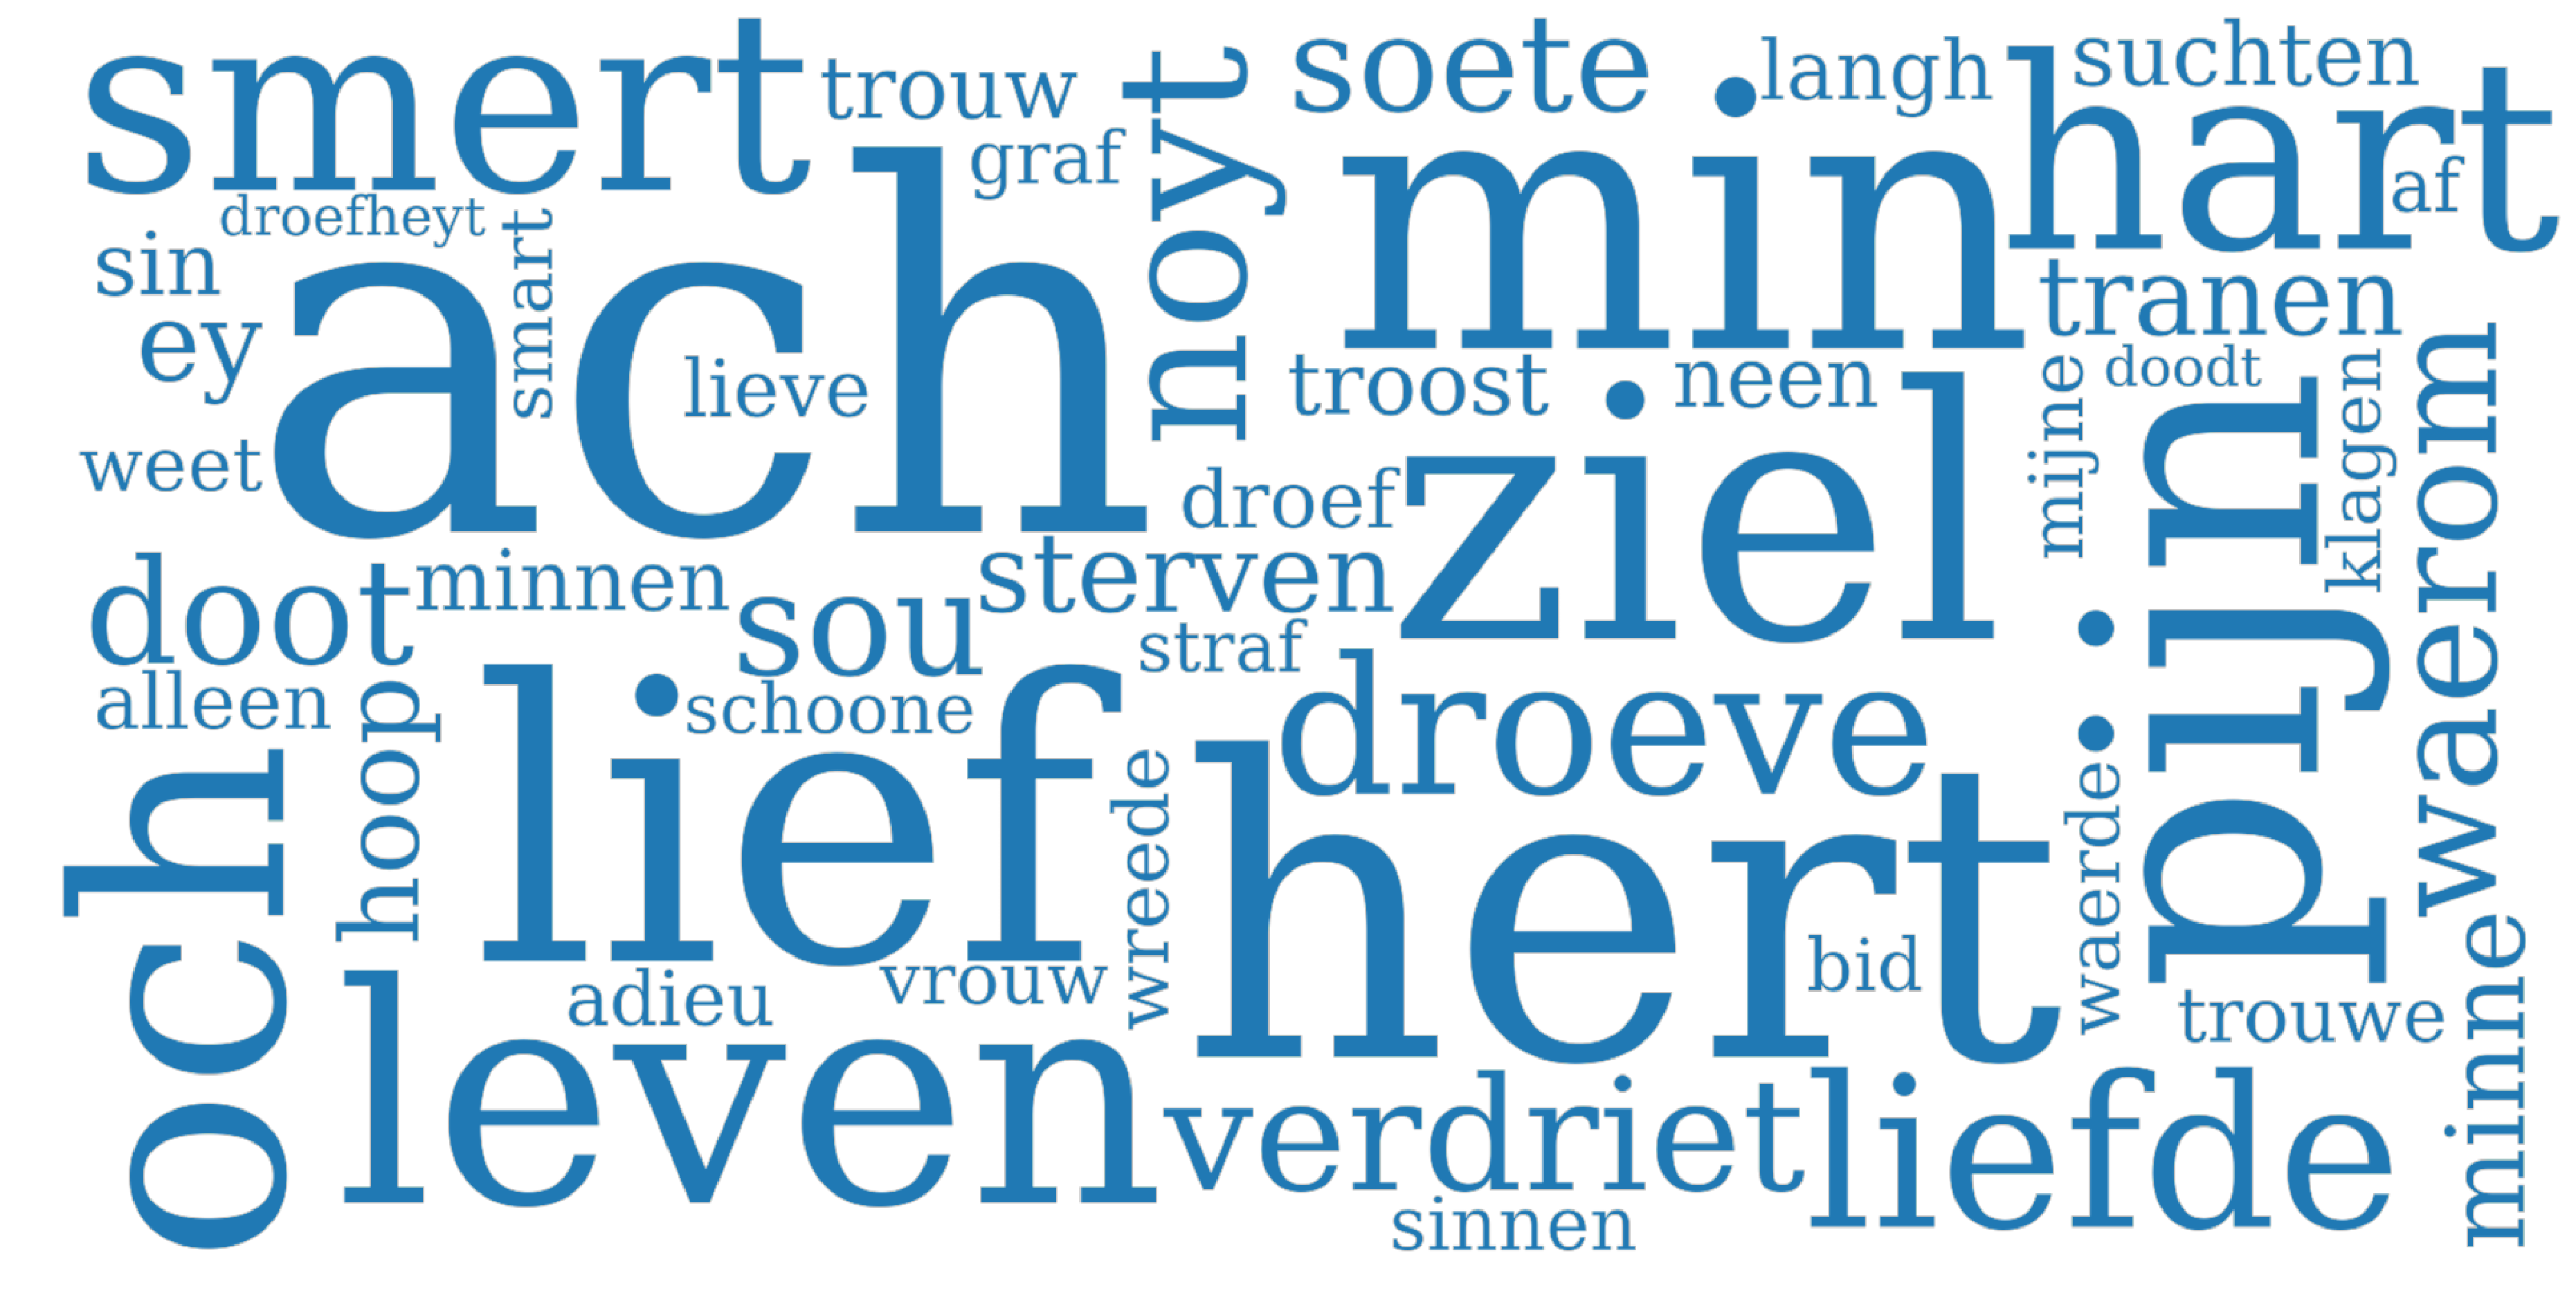
\includegraphics[width=\linewidth]{original_topic3}
		\caption{\textit{love \& sadness} (3)}
		\label{fig:topic3Original}
		\vspace{4ex}
	\end{minipage}%%
	\begin{minipage}[c]{0.48\linewidth}
		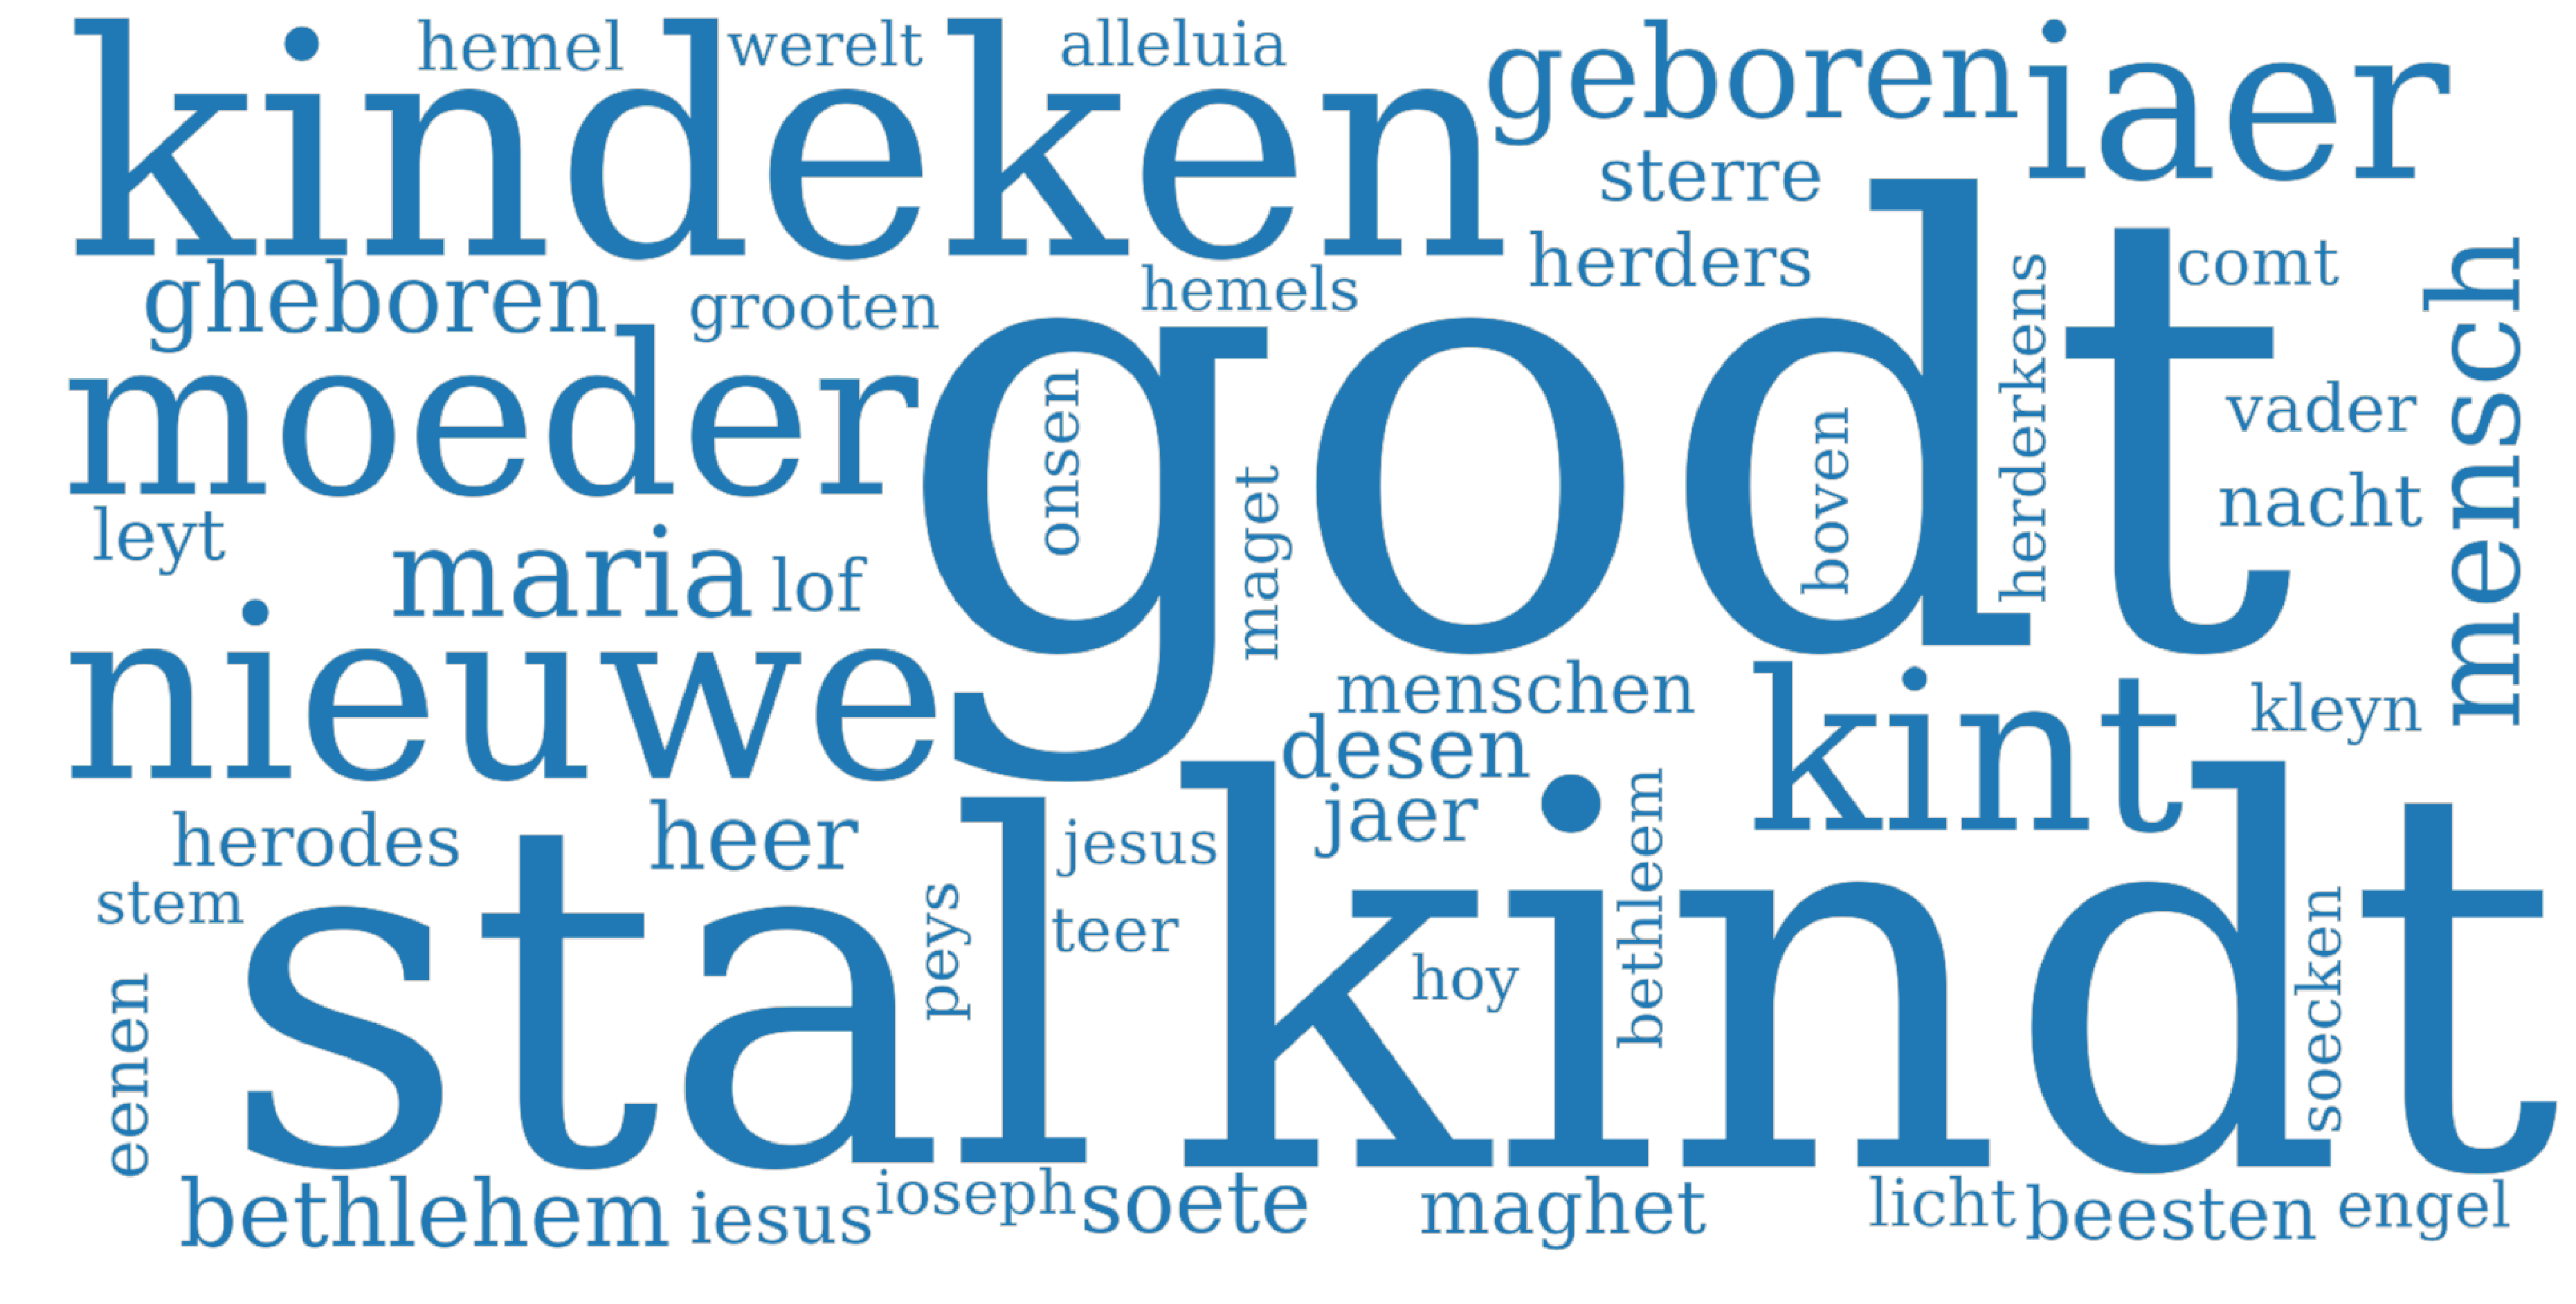
\includegraphics[width=\linewidth]{original_topic7}
		\caption{\textit{Christmas} (7)}
		\label{fig:topic7Original}
		\vspace{4ex}
	\end{minipage}%%
	\hfill
	\begin{minipage}[c]{0.48\linewidth}
		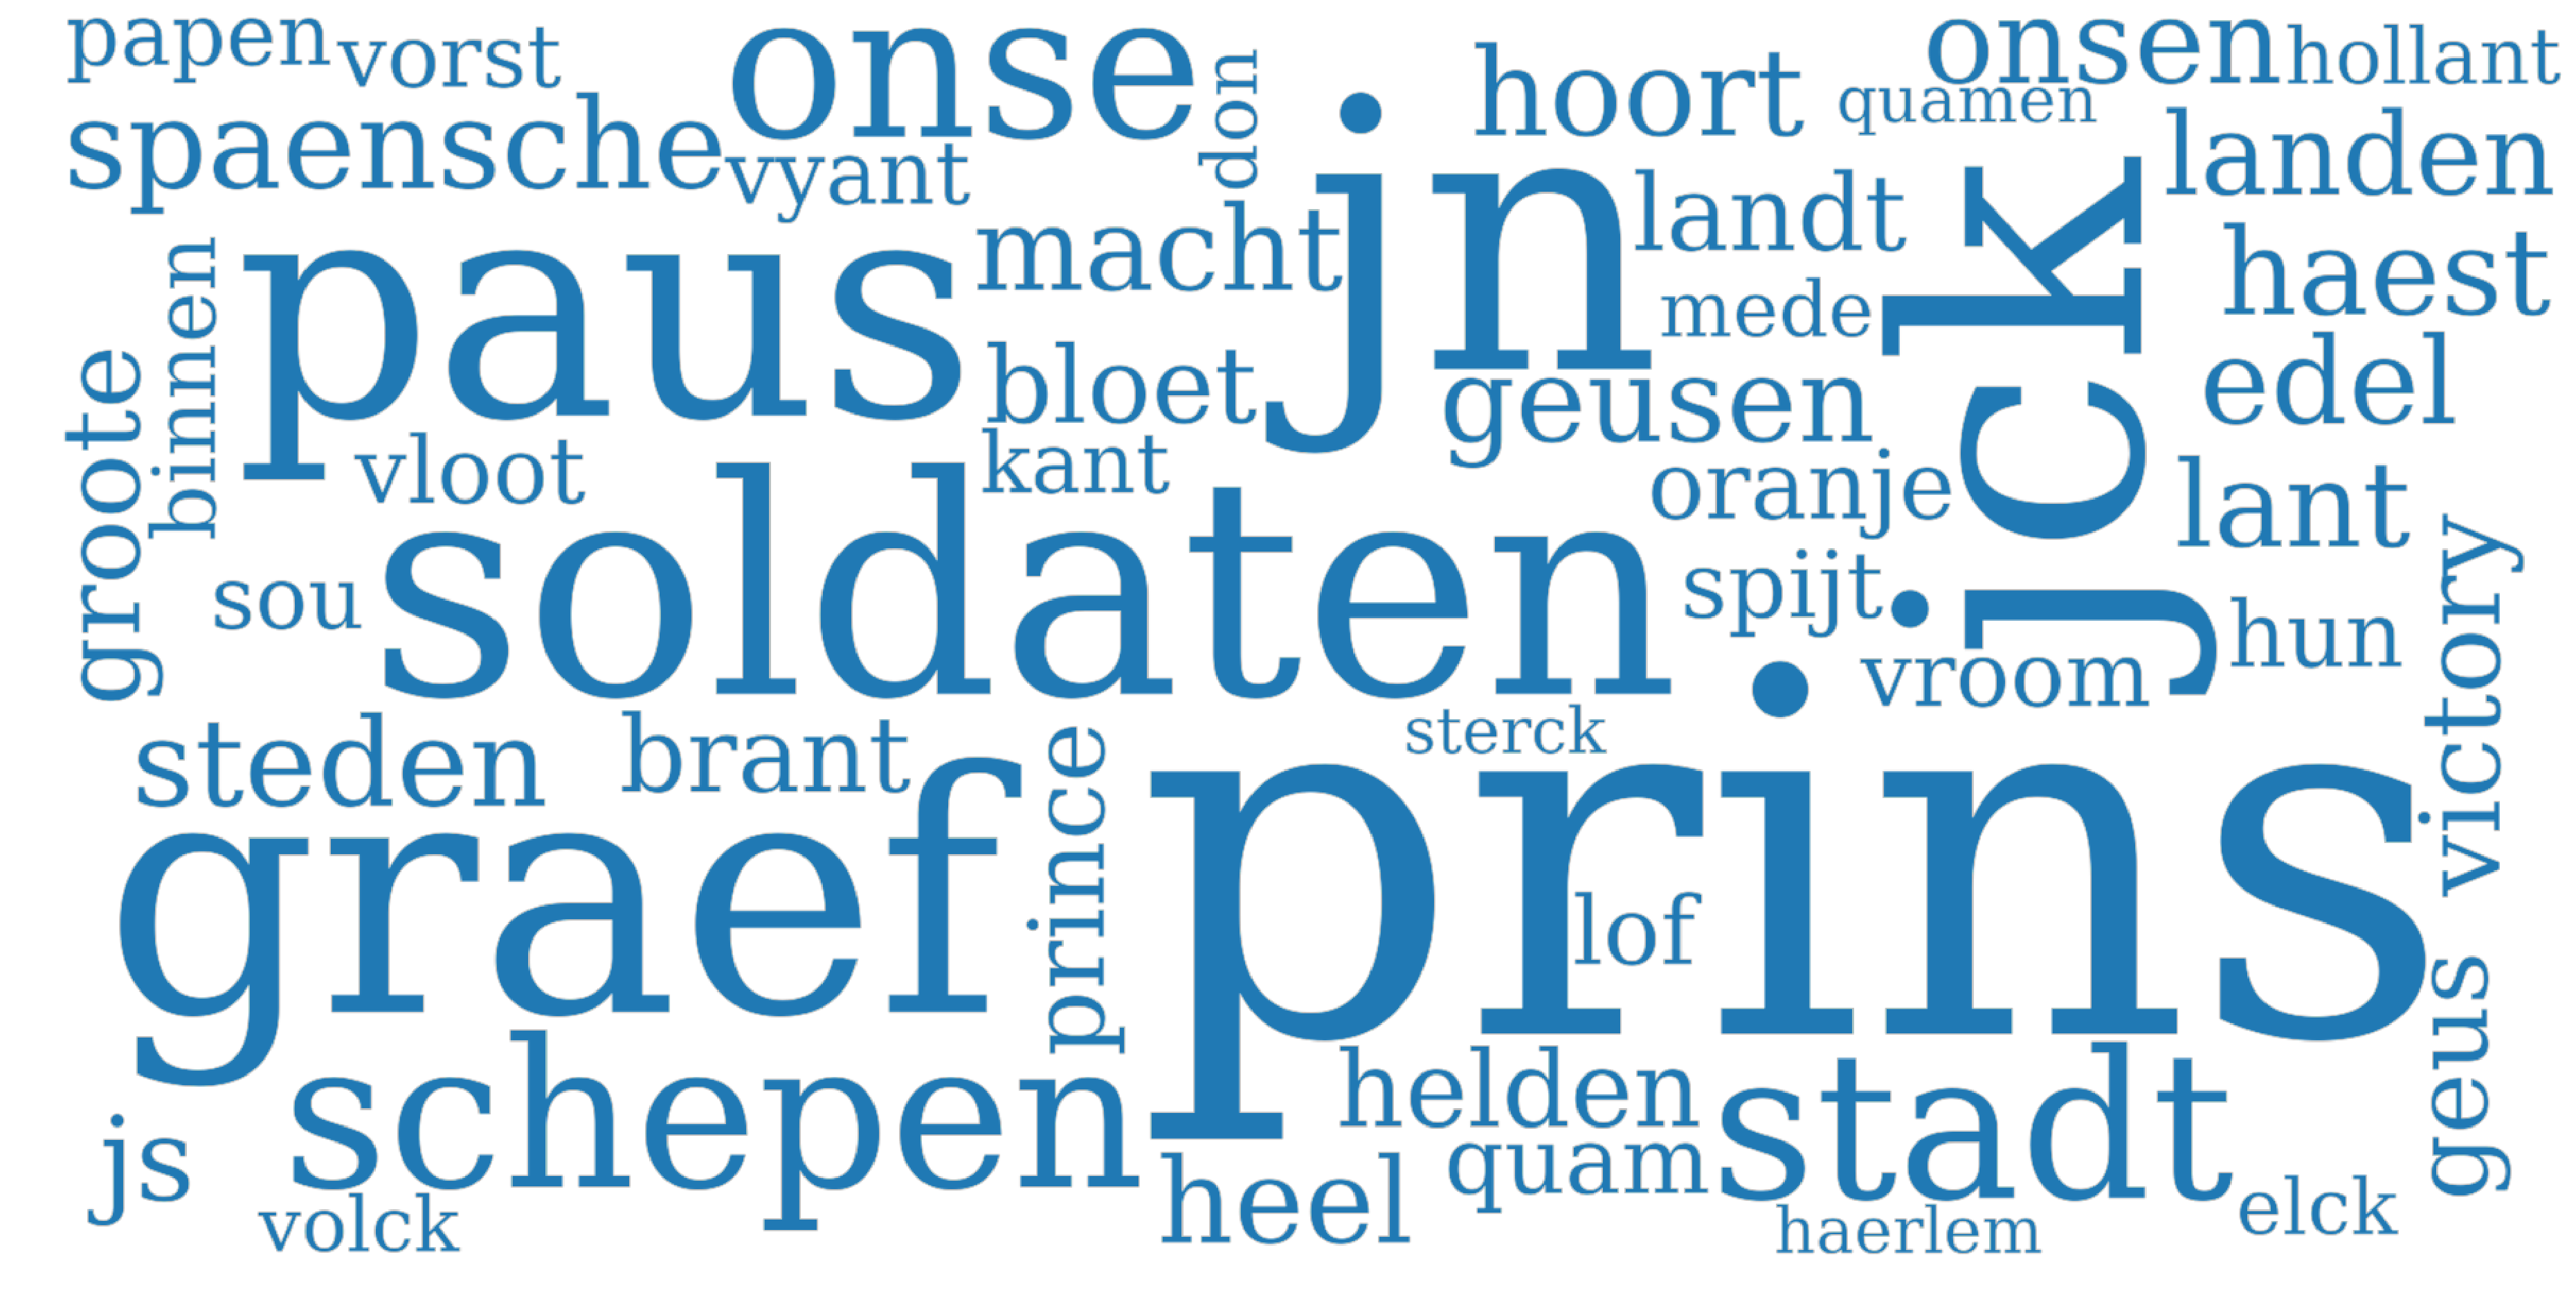
\includegraphics[width=\linewidth]{original_topic10}
		\caption{\textit{nation \& country} (10)}
		\label{fig:topic10Original}
		\vspace{4ex}
	\end{minipage}%%
	\begin{minipage}[c]{0.48\linewidth}
		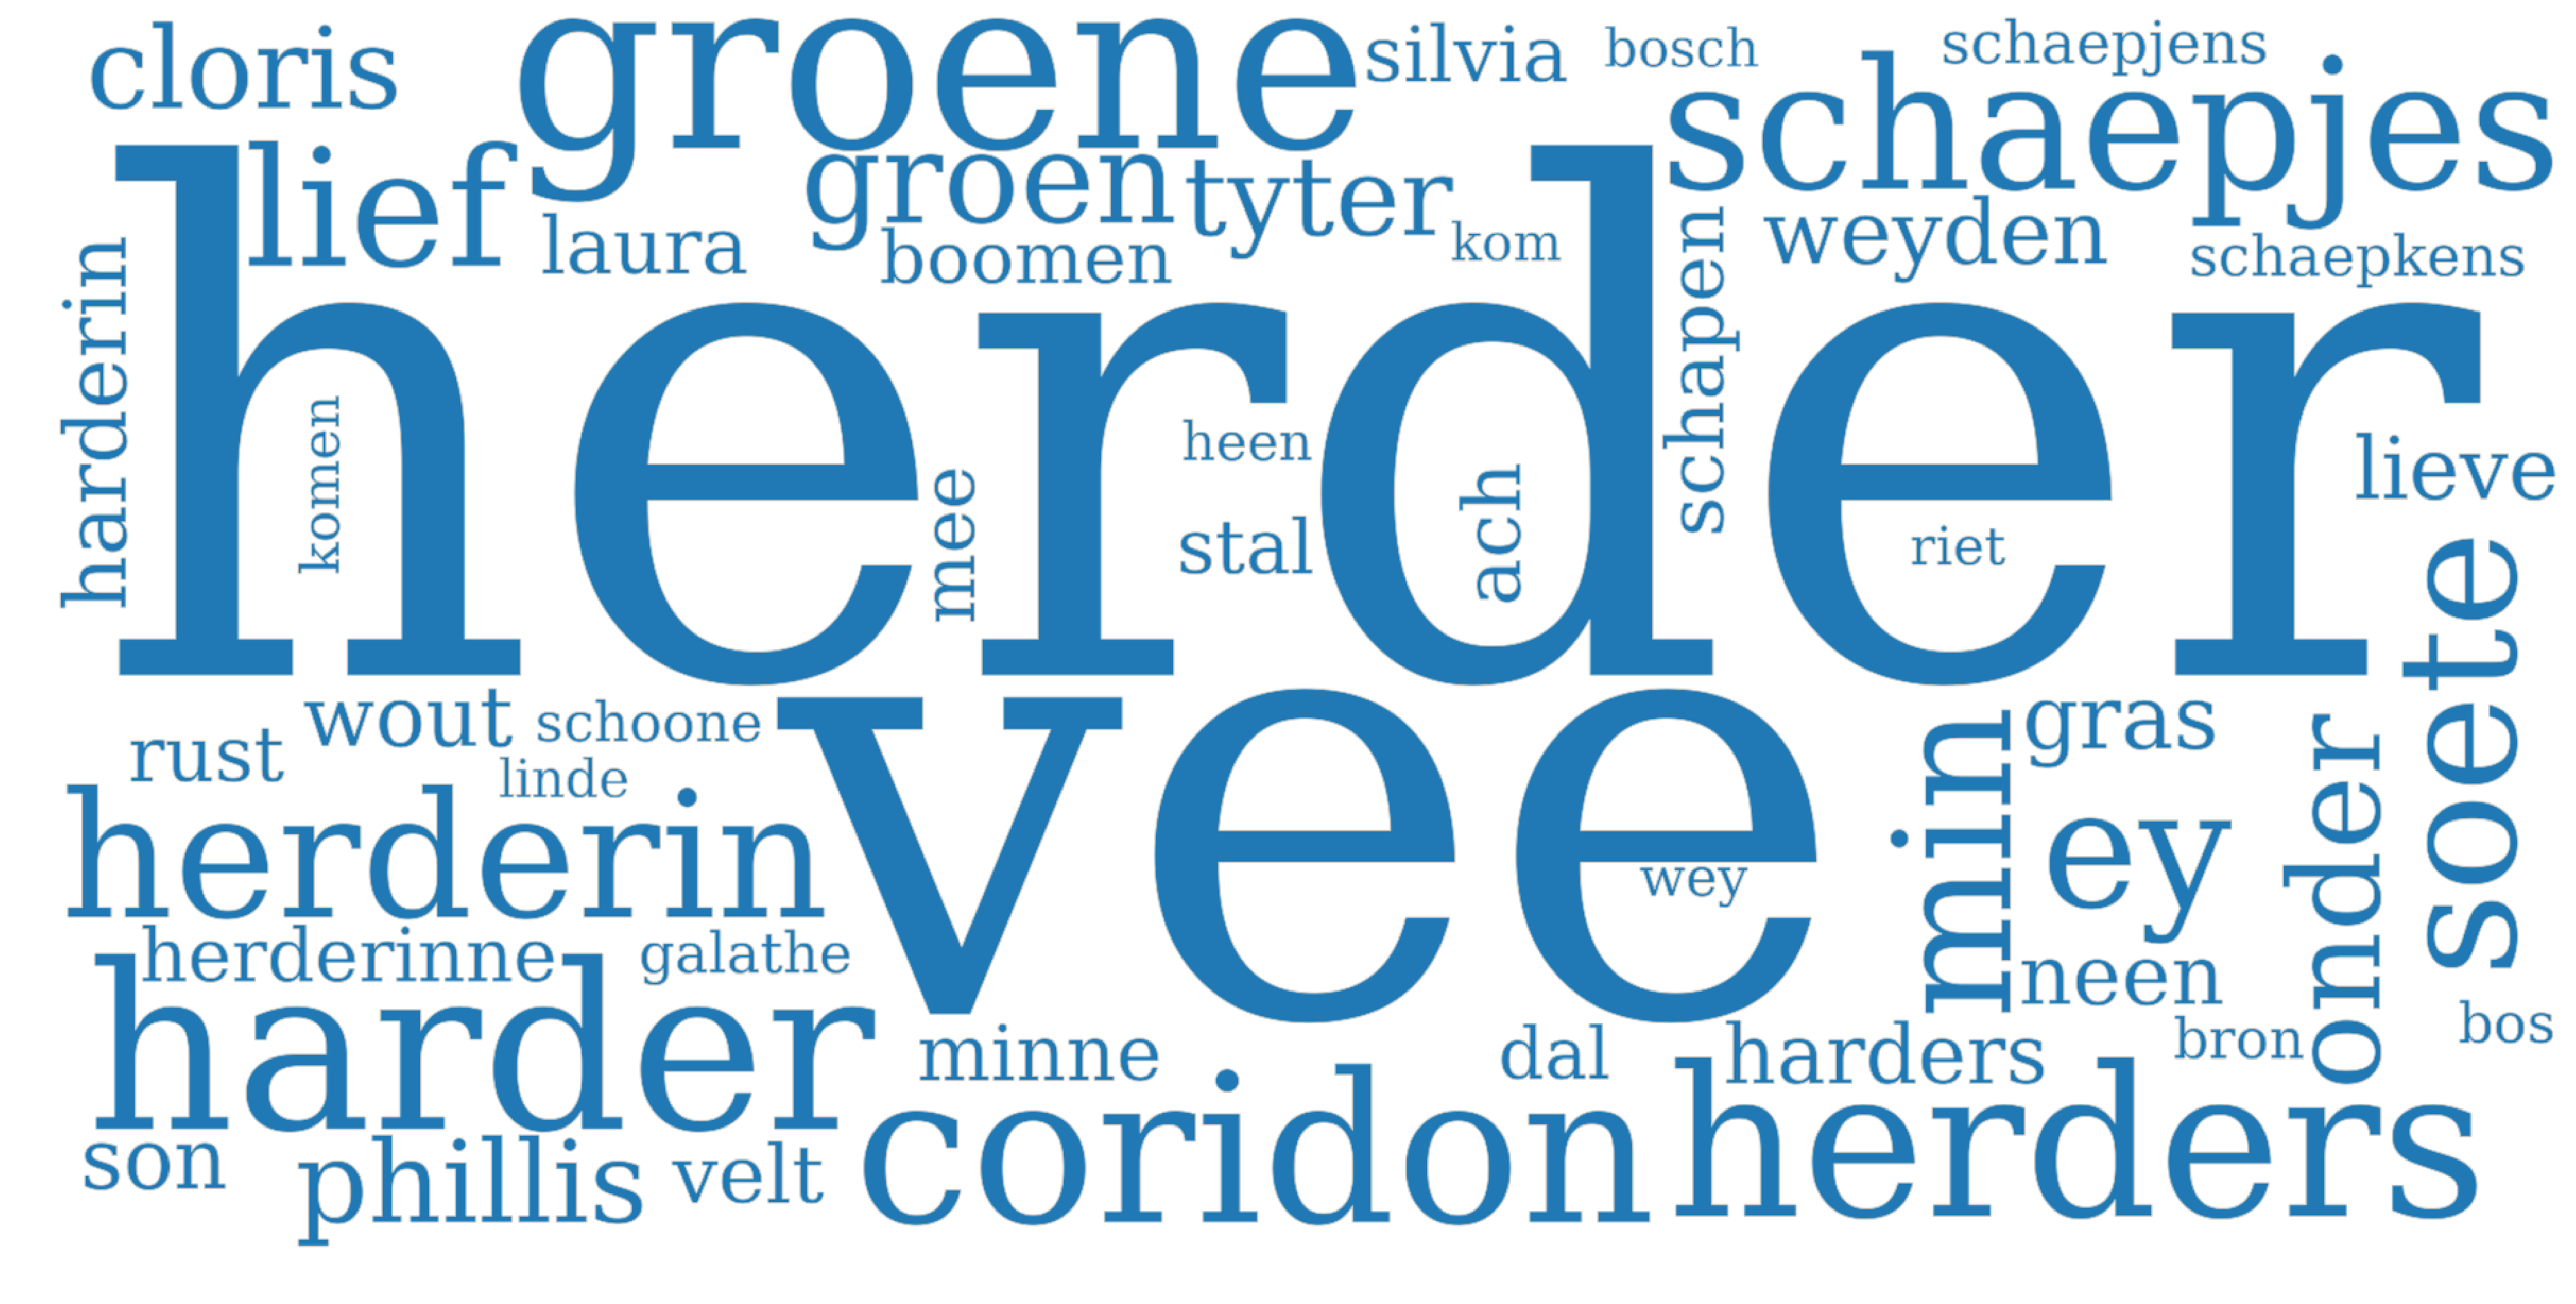
\includegraphics[width=\linewidth]{original_topic12}
		\caption{\textit{bucolic songs} (12)}
		\label{fig:topic12Original}
		\vspace{4ex}
	\end{minipage}%%
	\hfill
	\begin{minipage}[c]{0.48\linewidth}
		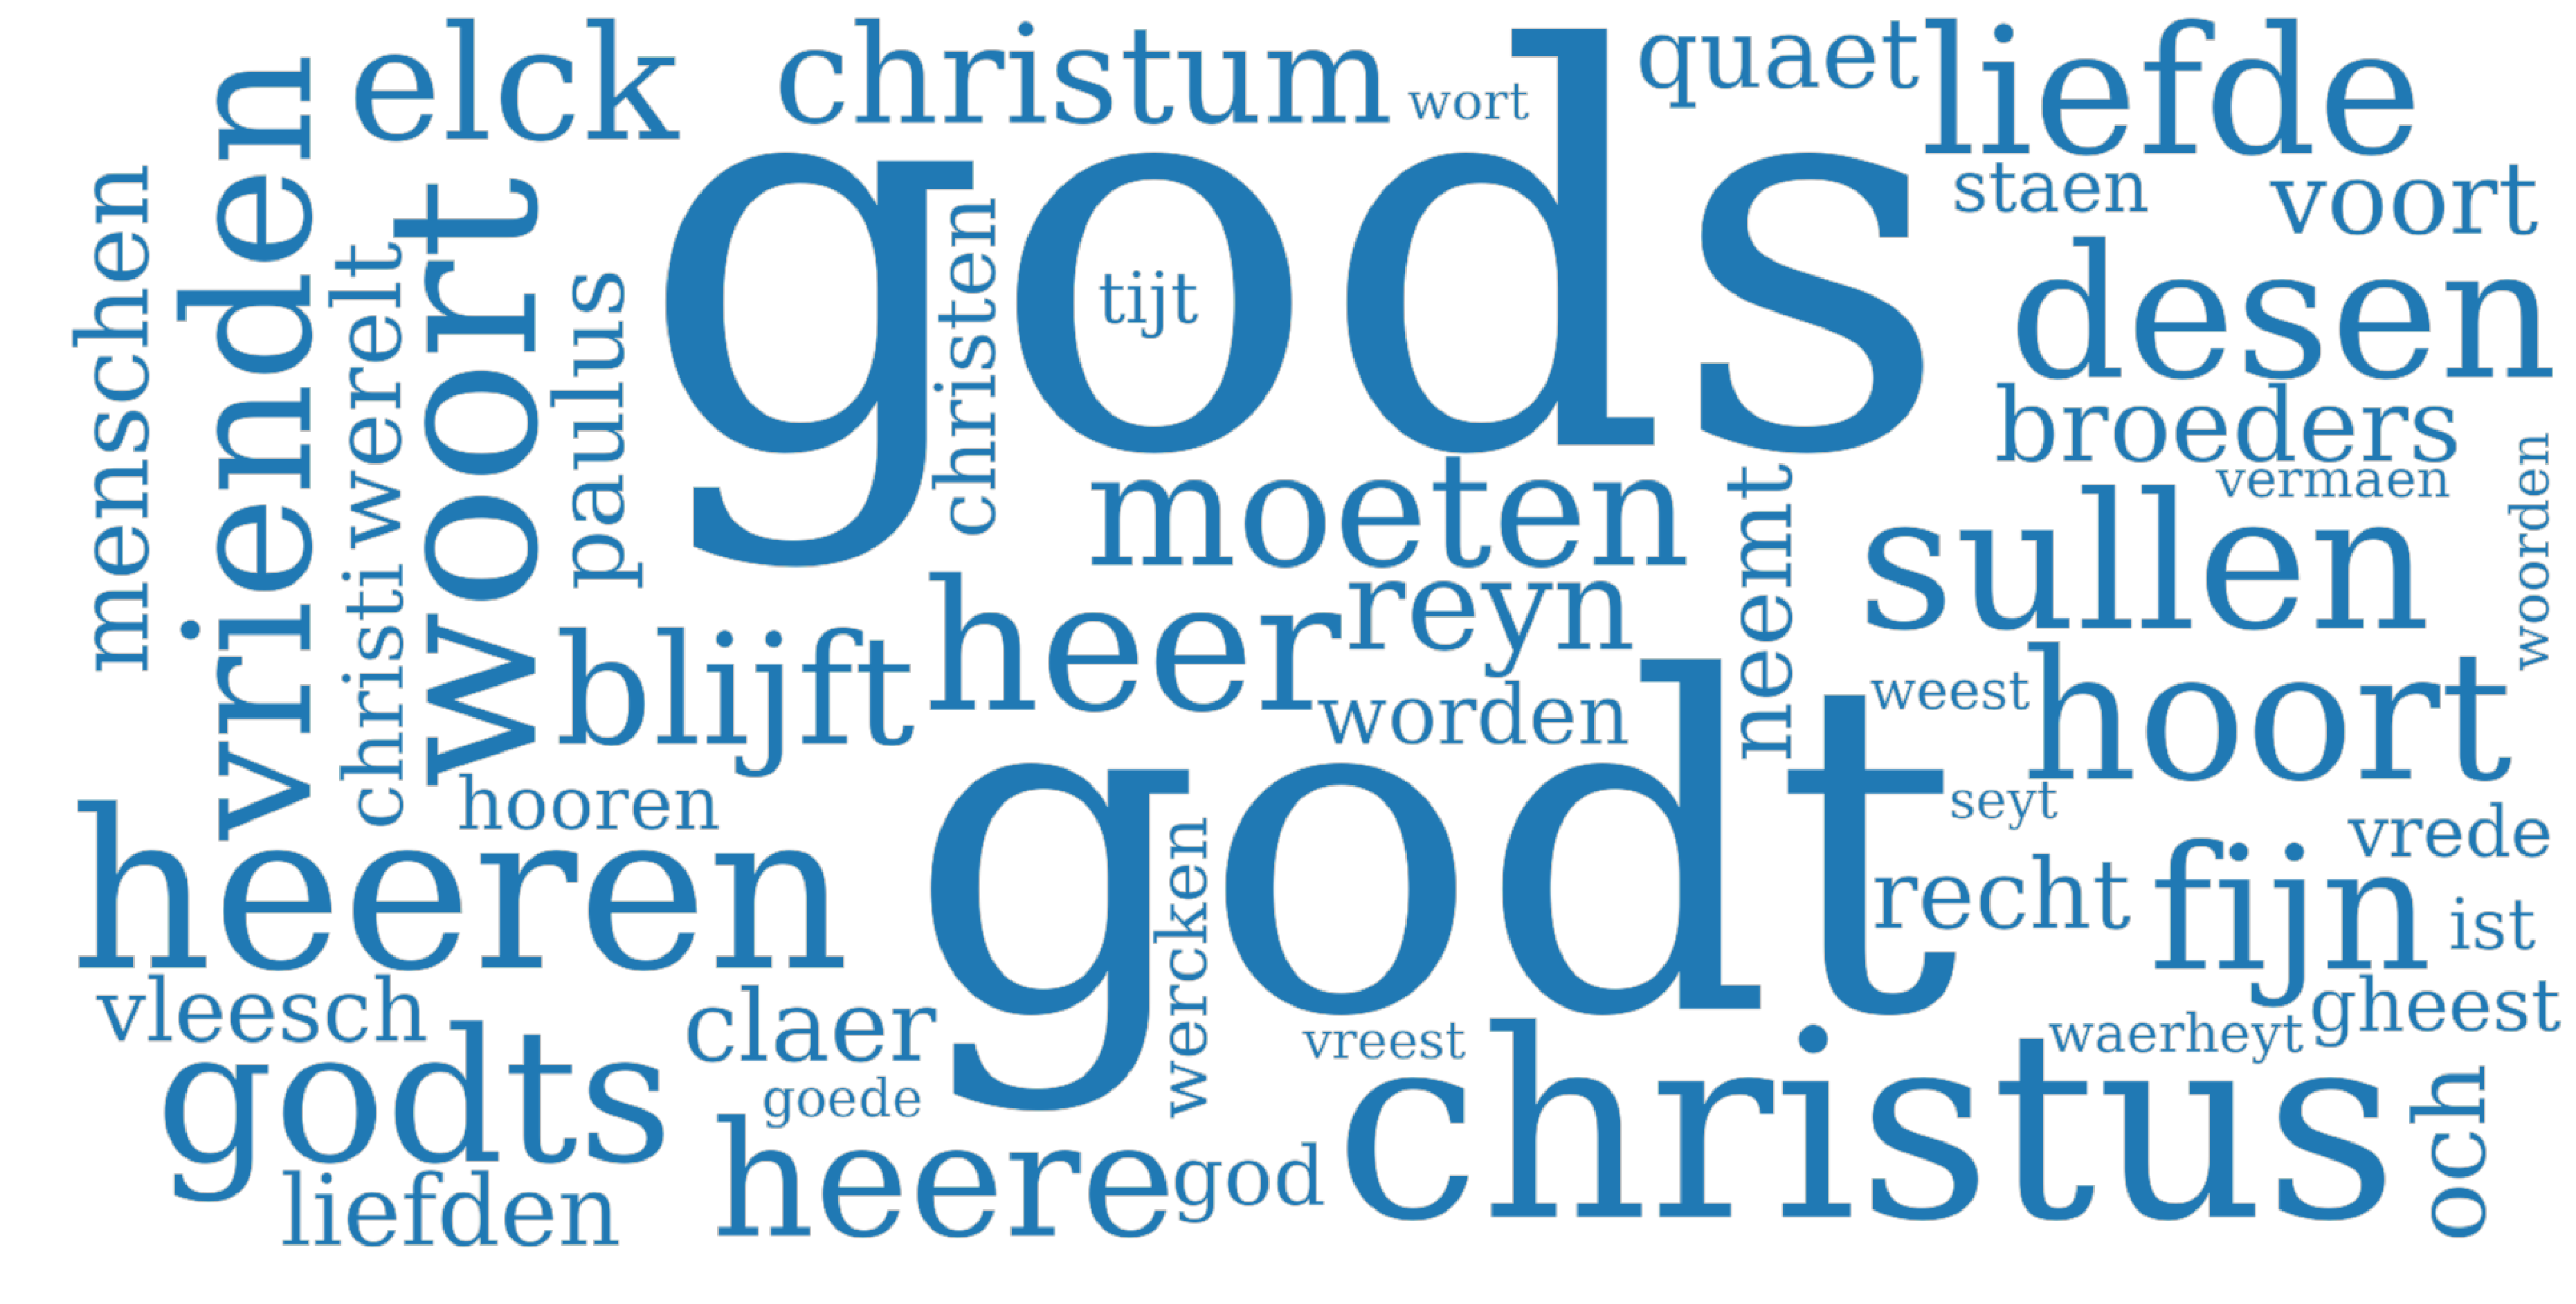
\includegraphics[width=\linewidth]{original_topic42}
		\caption{\textit{religion \& happiness} (42)}
		\label{fig:topic42Original}
		\vspace{4ex}
	\end{minipage}%%
	\begin{minipage}[c]{0.48\linewidth}
		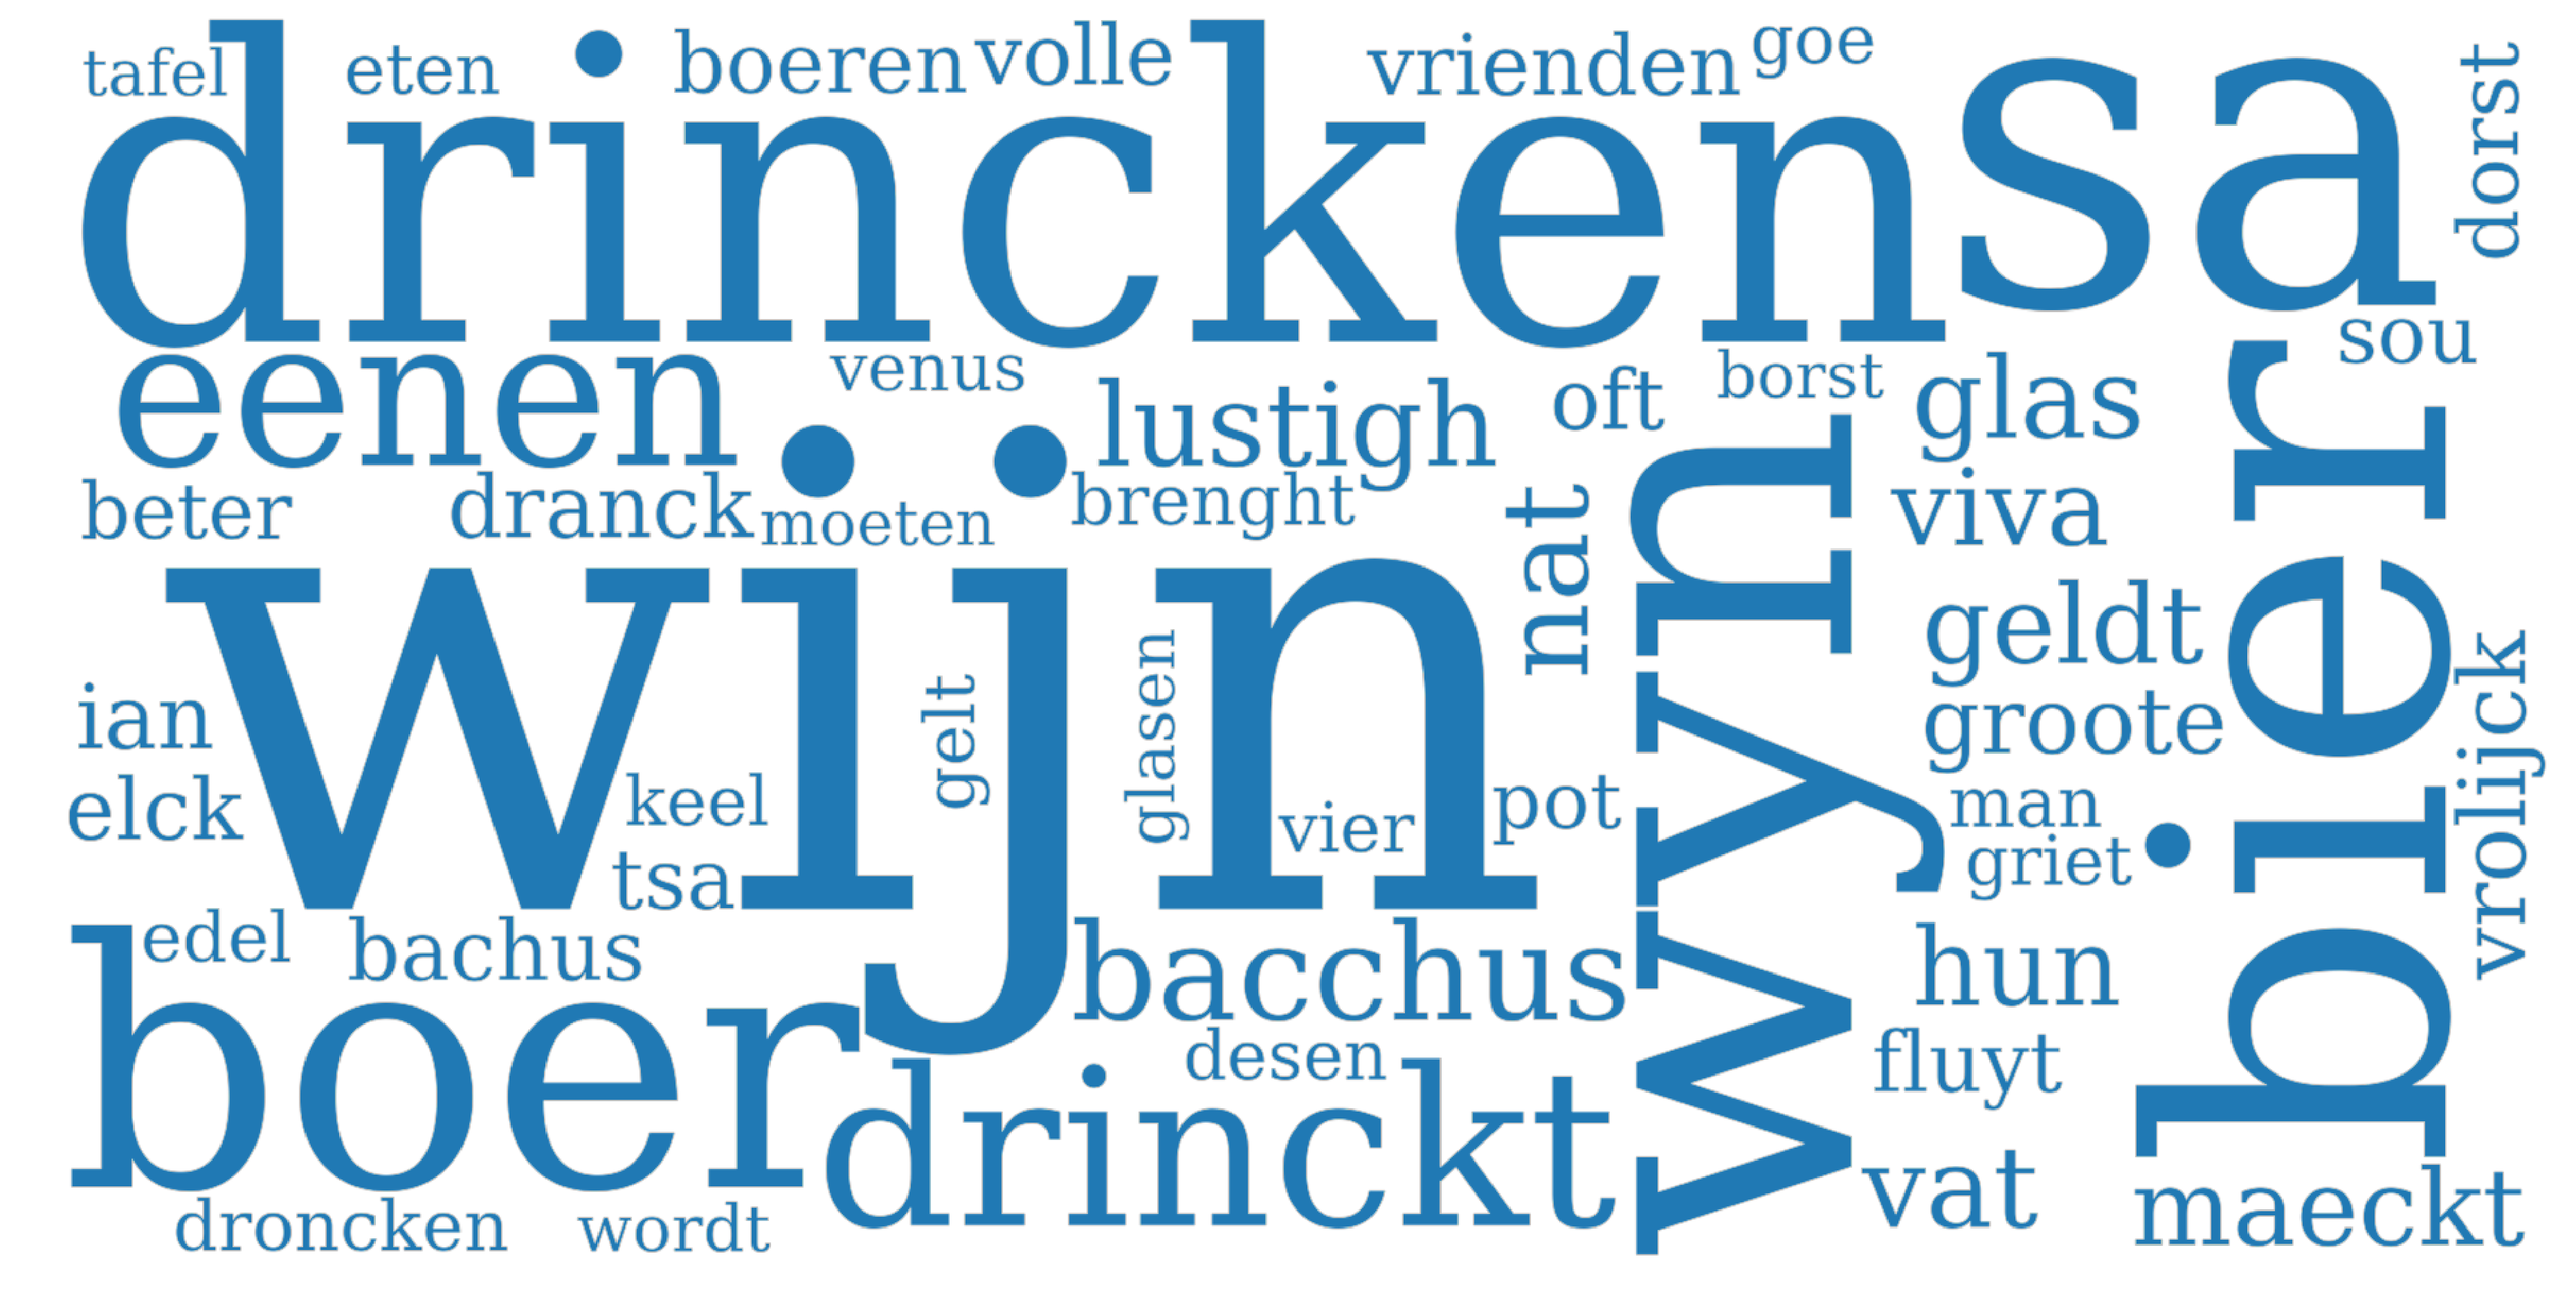
\includegraphics[width=\linewidth]{original_topic43}
		\caption{\textit{drinking} (43)}
		\label{fig:topic43Original}
		\vspace{4ex}
	\end{minipage}%%
	\hfill
	\begin{minipage}[c]{0.48\linewidth}
		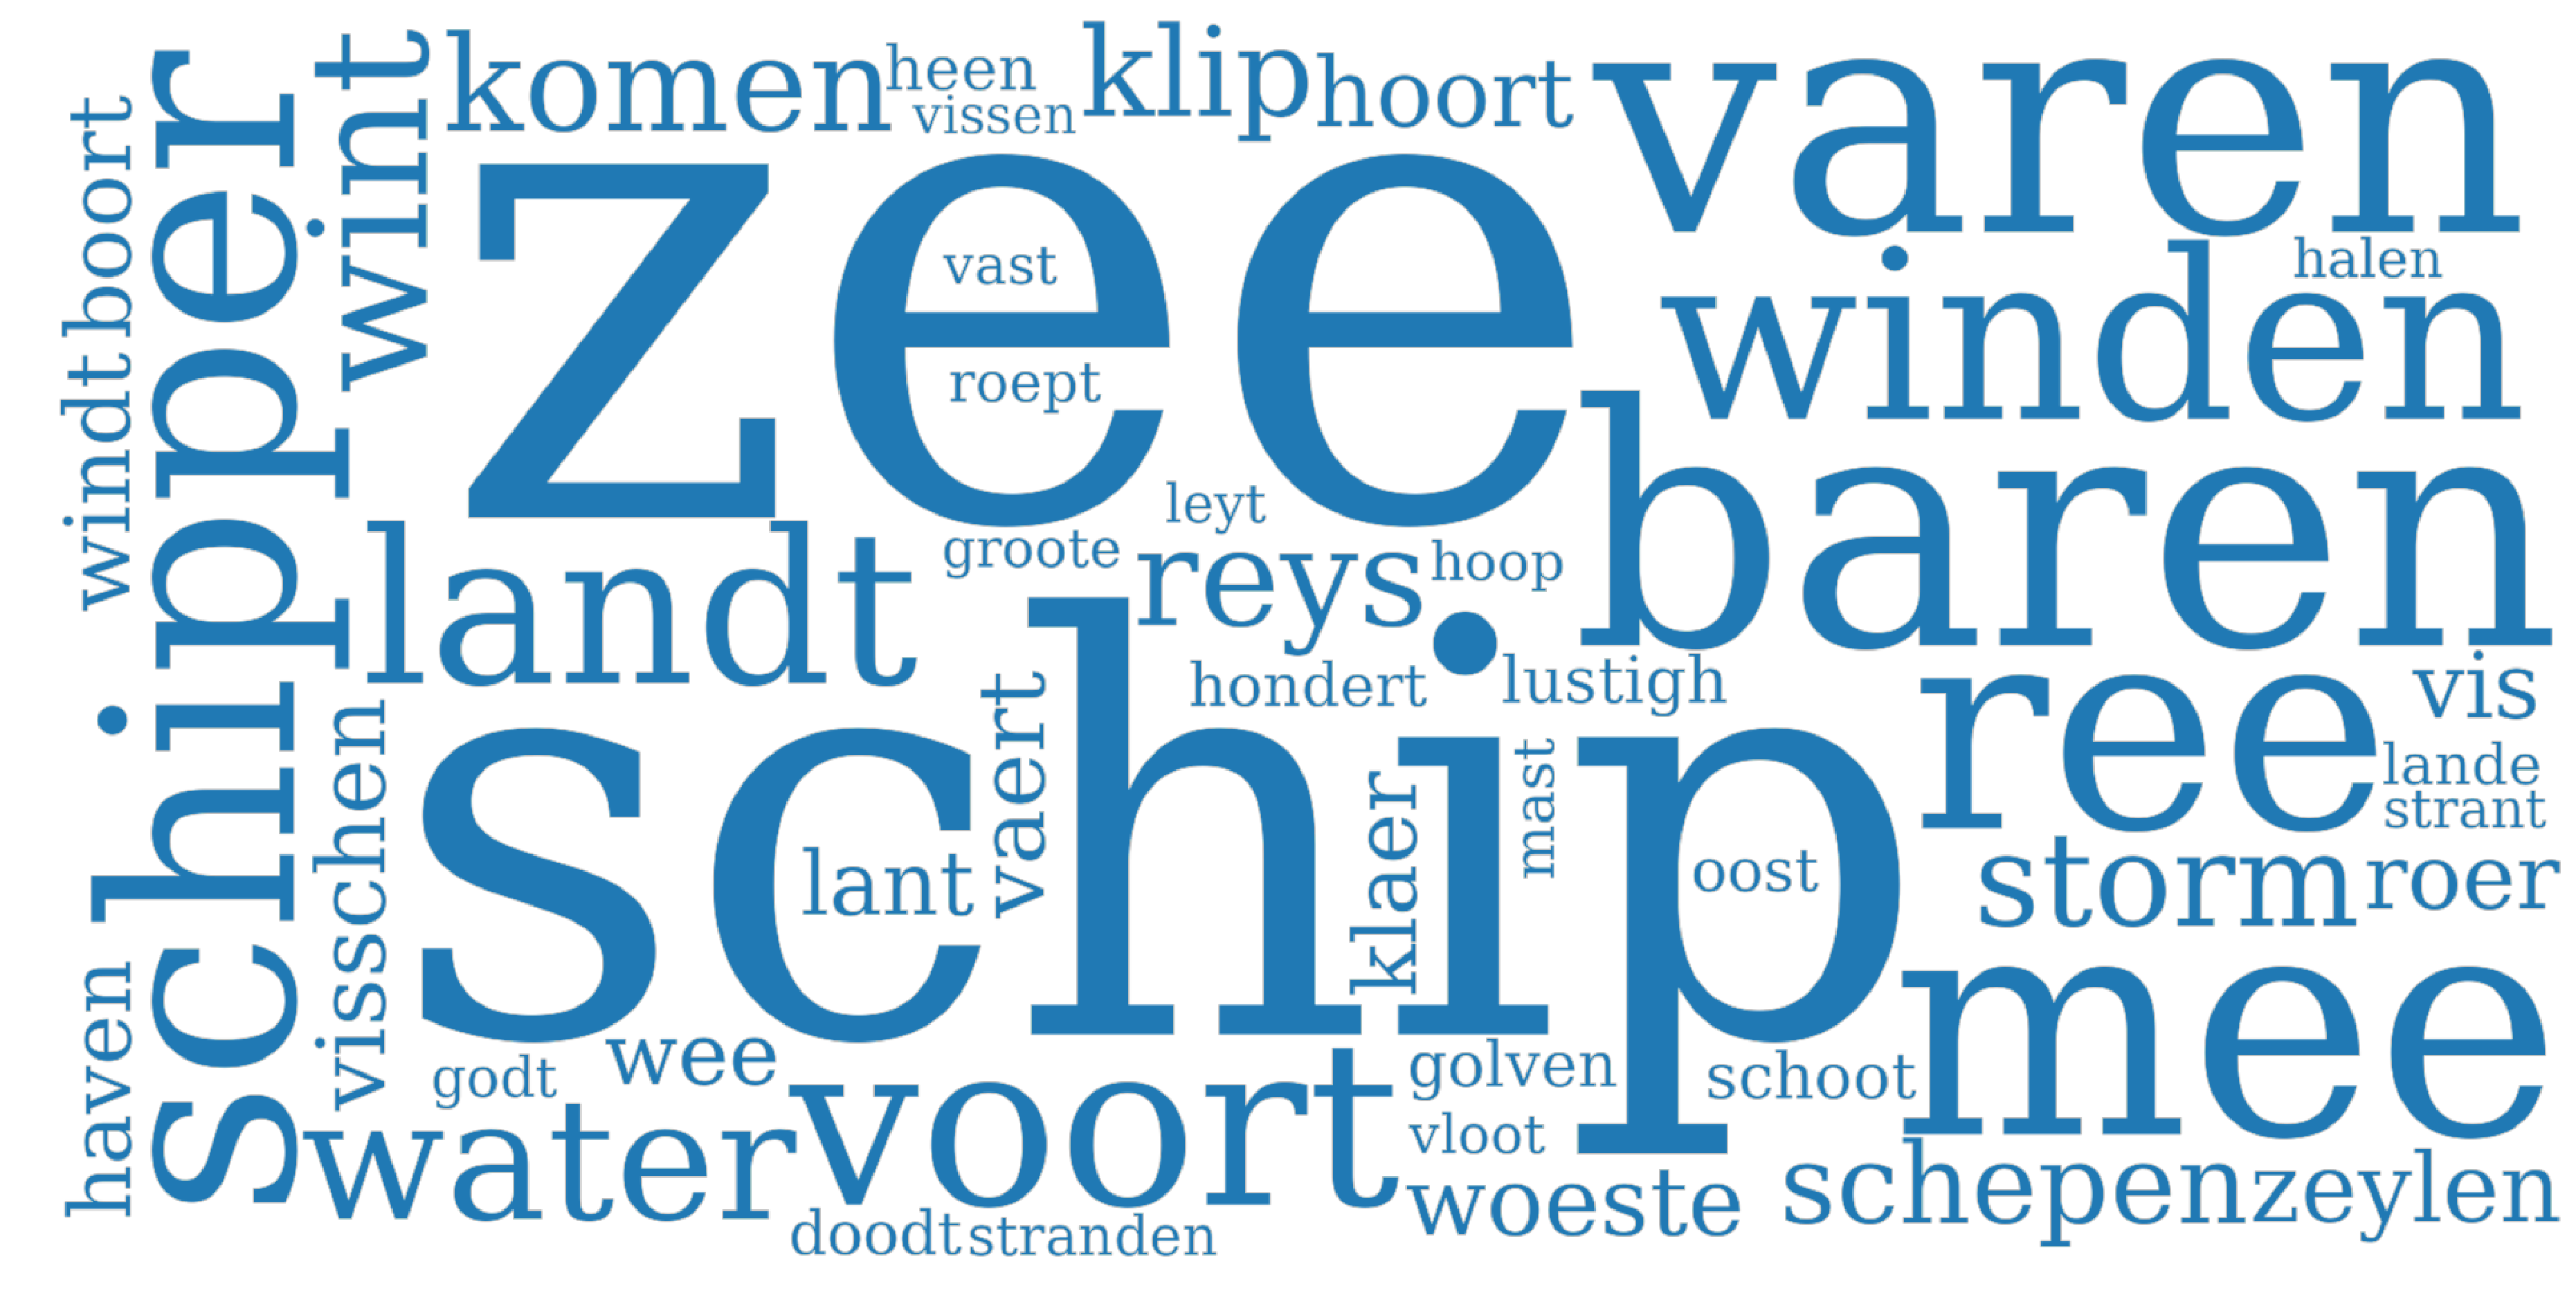
\includegraphics[width=\linewidth]{original_topic46}
		\caption{\textit{sea} (46)}
		\label{fig:topic46Original}
		\vspace{4ex}
	\end{minipage}%%
	\begin{minipage}[c]{0.48\linewidth}
		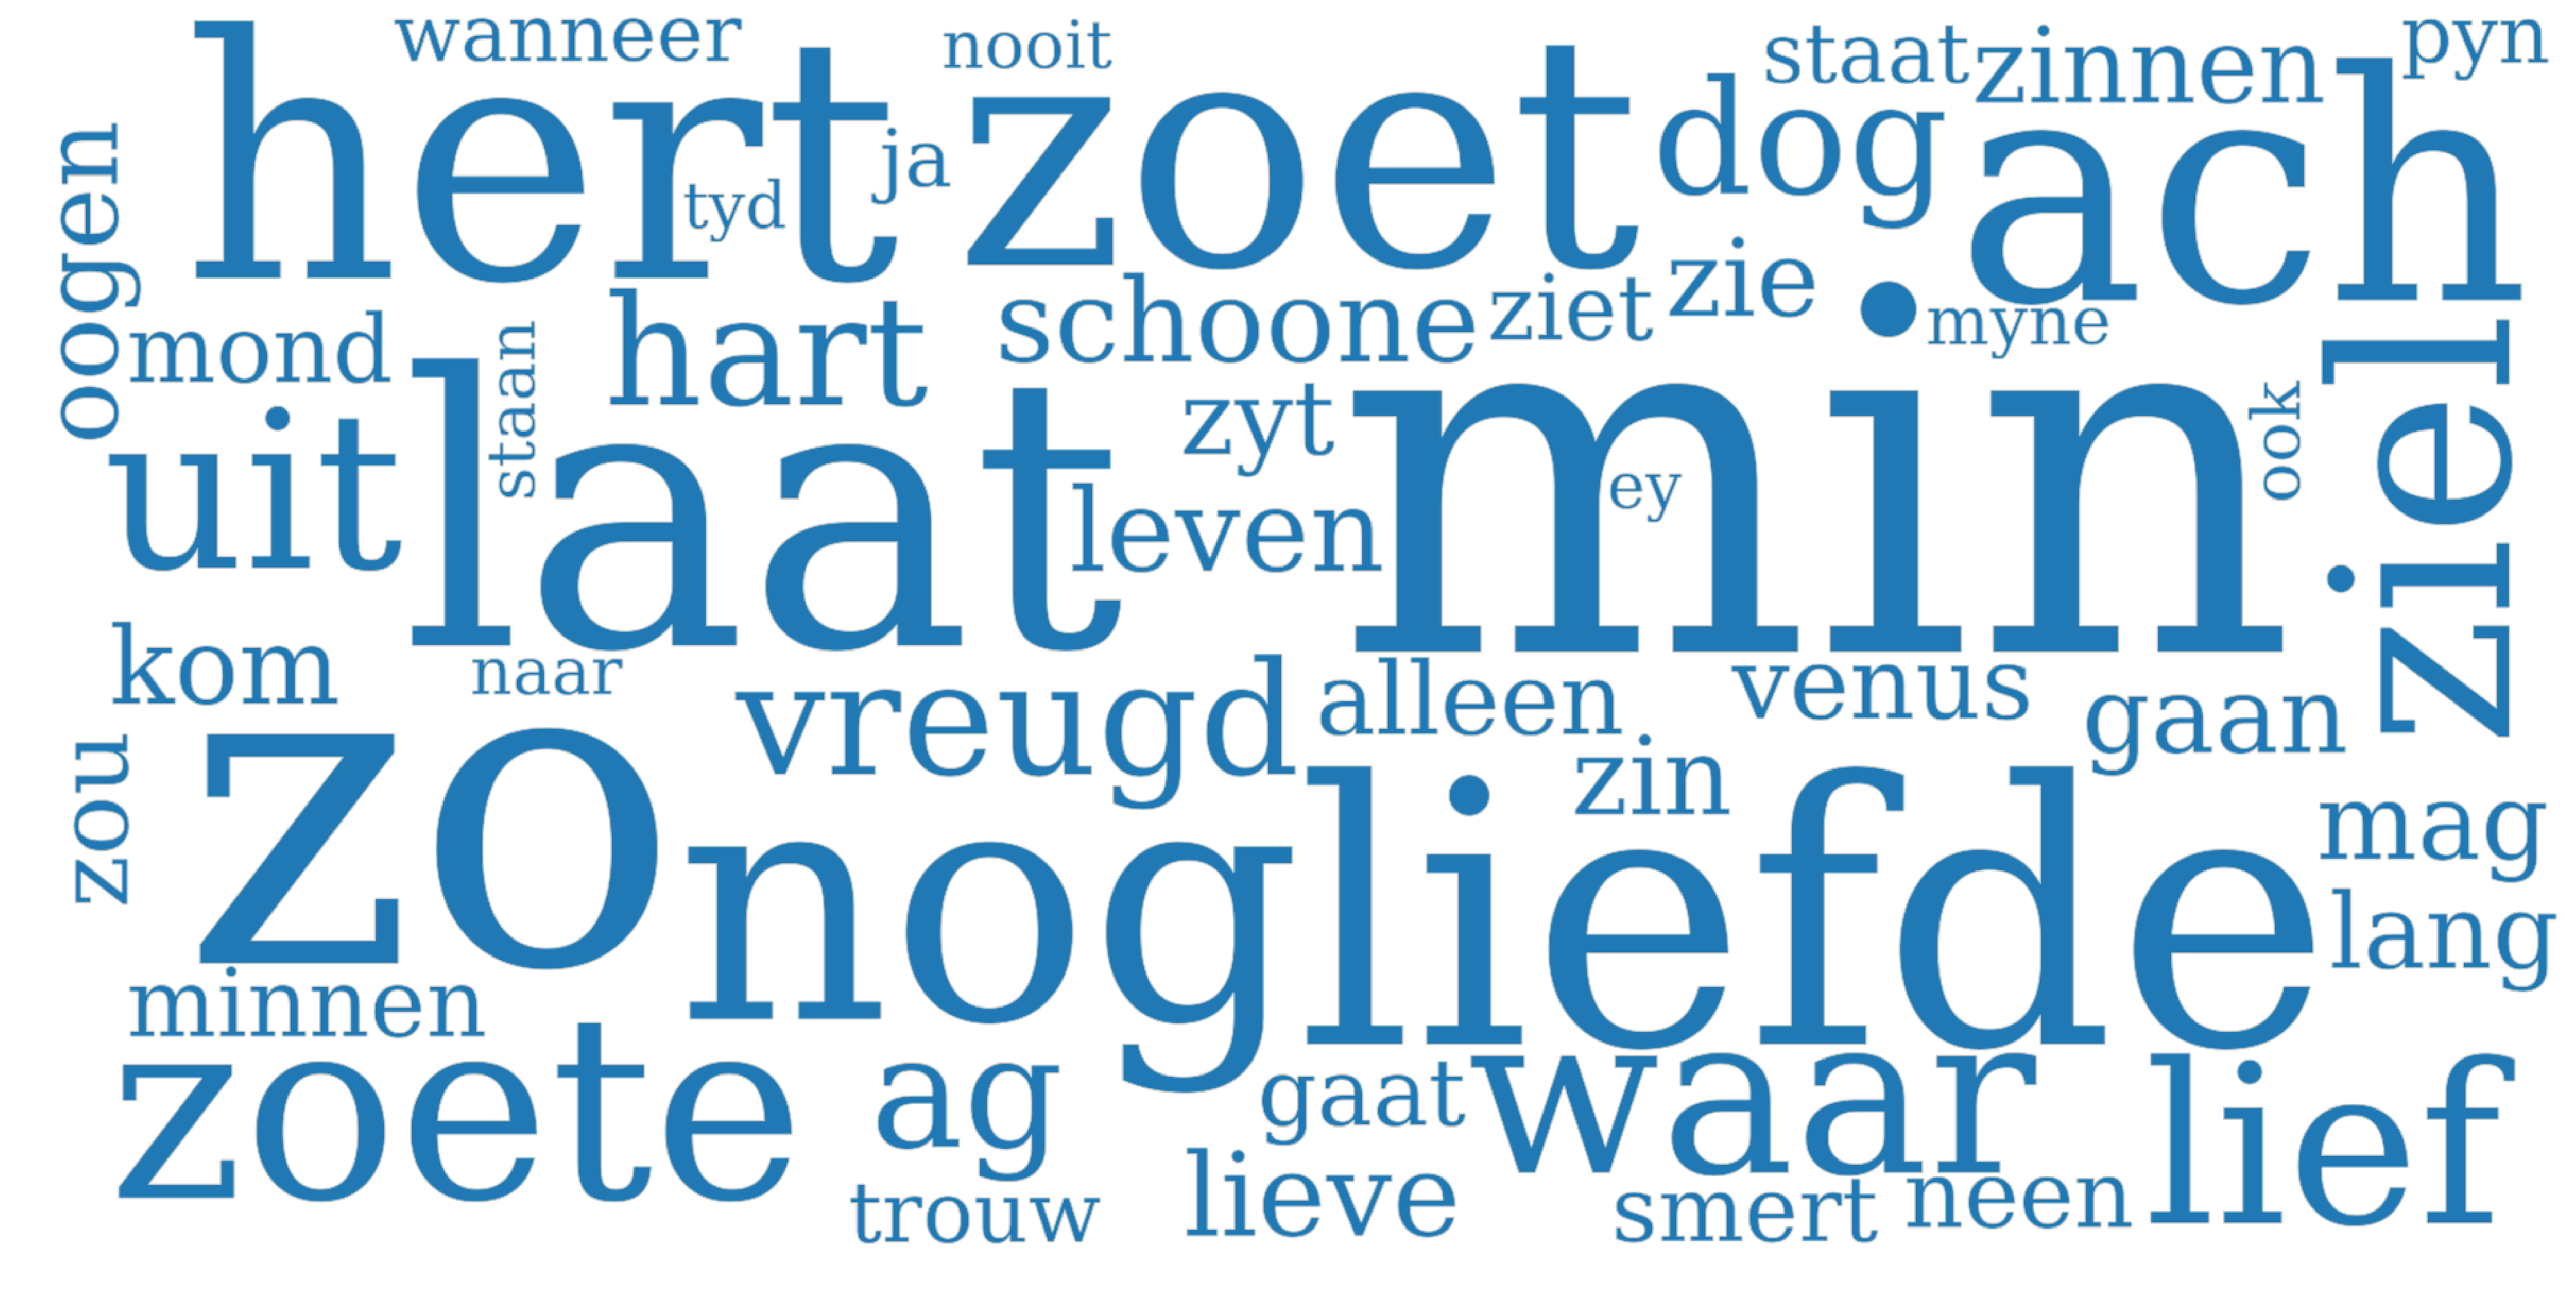
\includegraphics[width=\linewidth]{original_topic49}
		\caption{\textit{love \& happiness} (49)}
		\label{fig:topic49Original}
		\vspace{4ex}
	\end{minipage}%%
\end{figure}

Topic 7 (Figure~\ref{fig:topic7Original}) can easily be recognized as \textit{Christmas}, due to words as \enquote{kindeken}, \enquote{stal}, \enquote{maria}, \enquote{bethlehem}, \enquote{geboren} and \enquote{kindt}. To topic 10 (Figure~\ref{fig:topic10Original}), I refer with \textit{nation \& country}: the words \enquote{prins}, \enquote{soldaten}, \enquote{geusen} and \enquote{oranje} leave no doubt that these are words from political songs. In topic 12 (Figure~\ref{fig:topic12Original}), words from pastoral or bucolic poetry are clustered: many words refer to the shepherd life, such as \enquote{herder}, \enquote{vee} and \enquote{schaepjes}. Less prominent, but still present in this topic, is the name \enquote{laura} and the words \enquote{lieve} and \enquote{lief}, which suggests that not only the love for nature is chanted in these songs. I assign the subject \textit{bucolic songs} to this topic. Topic 42 (Figure~\ref{fig:topic42Original}) seems a very general religious topic with words as \enquote{gods}, \enquote{godt}, \enquote{christus} and \enquote{heeren}, all be it that almost only positive emotions are mentioned: \enquote{reyn}, \enquote{fijn}, \enquote{liefde}, \enquote{vrienden} and \enquote{vrede}. Therefore I assign the subject \textit{religion \& happiness} to this topic. Topic 43 (Figure~\ref{fig:topic43Original}) can easily be recognized as \textit{drinking}. All kinds of references to drinking are clustered in this topic, such as \enquote{drincken}, \enquote{wijn}, \enquote{bier}, \enquote{droncken} and \enquote{glas}, accompanied by words as \enquote{bacchus} (the Roman god of the wine) and \enquote{viva}. In topic 46 (Figure~\ref{fig:topic46Original}) words that refer to the life on sea are found: \enquote{zee}, \enquote{schip}, \enquote{varen}, \enquote{winden} and \enquote{baren}. I assign the word \textit{sea} to this topic. To the groups of words that are not depicted here in word clouds, I assigned a topic as well. It turns out that a lot of topics have something to do with religion. This is not surprising at all, since Table~\ref{table:SongsCat} already showed that almost 40\% of the corpus are songs from the category \enquote{religion}. In some cases it is quite easy to determine a certain subcategory (such as \textit{religion \& eternity}, \textit{religion \& happiness}, \textit{ religion \& sin}), but for a lot of religious topics the difference is not easy to distinguish.

However, I do not know yet which topics are more dominant in the corpus than the others. Each song receives a distribution over all the topics. This means that, for each song,  the sum of contributions of topics is always 1. Ideally, there is for each song one topic which is way more dominant than the 49 others. To see which topics are the most dominant in my corpus, I choose for each song the topic that has the highest contribution, using the following code:

\begin{lstlisting}
	transformed_docs = lda.load_document_topics()
	docs = [[texts[i]] + [r[0] for r in list(zip(max(row, key=lambda x:x[1])))] for i, row in enumerate(transformed_docs)]
	dominant_topics = pd.DataFrame(docs, columns=["document_id", "dominant_topic", "perc_contribution"])
\end{lstlisting}

\begin{table}
	\begin{minipage}{0.5\textwidth}
		\begin{tabular}{ccl}
			\toprule
			Topic & Songs & Subject \\
			\midrule
			49             &  1377 & love \& happiness \\
			3              &  1078 & love \& sadness \\
			21             &   993 & religion \& eternity \\
			0              &   993 & religion \\
			40             &   962 & religion \& emotions \\
			24             &   787 & religion \\
			42             &   770 & religion \& happiness \\
			13             &   753 & rejection \\
			30             &   704 & religion \\
			18             &   703 & ??? \\
			26             &   698 & virtuous life \\
			32             &   695 & physical love \\
			25             &   646 & religion \\
			4              &   643 & religion \& praise \\
			39             &   637 & verbs \\
			29             &   579 & love \& consolation \\
			9              &   511 & religion \\
			23             &   483 & religion \& sin \\
			15             &   429 & religion \& virtues \\
			28             &   413 & religion \\
			27             &   403 & death \& passion\\
			7              &   389 & Christmas \\
			12             &   381 & bucolic songs \\
			44             &   365 & religion \\
			22             &   351 & religion \\
			\vdots & \vdots & \vdots \\
			\bottomrule
		\end{tabular}
	\end{minipage} \hfill
	\begin{minipage}{0.5\textwidth}
		\begin{tabular}{|ccl}
			\toprule
			Topic & Songs & Subject \\
			\midrule
			\vdots & \vdots &\vdots \\
			
			43             &   350 & drinking \\
			19             &   338 & religion \\
			1              &   337 & religion \& Mary \\
			41             &   328 & love \& happiness \\
			8              &   315 & love \\
			48             &   305 & profane love \\
			31             &   265 & marriage \\
			14             &   262 & verbs \\
			10             &   250 & nation \& country \\
			36             &   248 & verbs \\
			38             &   246 & nature \\
			35             &   244 & religion \\
			11             &   241 & religion \\
			20             &   238 & German/French \\
			33             &   219 & God \& nation \\
			2              &   197 & God \& church \\
			47             &   178 & old spelling \\
			6              &   163 & ??? \\
			46             &   144 & sea \\
			16             &   133 & pronouns \\
			37             &   125 & Old Testament \\
			17             &   116 & love \& Jesus \\
			45             &   113 & ??? \\
			34             &   110 & trash \\
			5              &    89 & verbs \\
			\bottomrule
		\end{tabular}
	\end{minipage}
	\caption{Dominant topics in original corpus (\textit{n} = 22,297)}
	\label{table:DomTopOr}
\end{table}

\noindent Subsequently, I group the dominant topics and count how many times they appear in the dataframe \texttt{dominant\_topics}:

\begin{lstlisting}
topic_counts = dominant_topics["dominant_topic"].value_counts()
topic_contribution = round(topic_counts/topic_counts.sum(), 4)
df_dominant_topics = pd.concat([topic_counts, topic_contribution], axis=1)
df_dominant_topics.columns = ["Num_Documents", "Perc_Documents"]
\end{lstlisting}

\noindent The results are stored in Table~\ref{table:DomTopOr}. It is important to realize that the sum of songs in this table is 22,297, which means that, for now, only the \enquote{original} songs are included, and not their reprints and appearances in other songbooks. That is a step I will take in a later stadium, after I have evaluated the three different models.

A tool that can help to get more insight in the topics and how they are related to each other, is the Python package \texttt{pyLDAvis}, which is a library for interactive topic model visualization. The package extracts information from a fitted LDA topic model to inform an interactive web-based visualization. In order to visualize my topic model, made with the MALLET wrapper of \texttt{gensim}, I first have to convert it to a \enquote{normal} LDA model in \texttt{gensim}. Afterwards, I import the converted model into the \texttt{pyLDAvis prepare}-function:

\begin{lstlisting}
model = gensim.models.wrappers.ldamallet.malletmodel2ldamodel(lda)

import pyLDAvis
import pyLDAvis.gensim

pyLDAvis.enable_notebook()
vis = pyLDAvis.gensim.prepare(model, corpus, dictionary, sort_topics=False)
\end{lstlisting}

\noindent With \texttt{sort\_topics=False}, I make sure that the same topics are used as the ones in the original model, made with \texttt{gensim.models.wrappers.LdaMallet}. The output is a so-called Intertopic Distance Map, with multidimensional scaling. The screenshot in Figure~\ref{fig:pyLDAvisOriginal} gives an impression how the interactive visualization looks like. Each bubble on the left-hand side plot represents a topic. The larger the bubble, the more prevalent the topic is. An important note is that \texttt{pyLDAvis} starts counting at 1, while the topics made with \texttt{gensim} start at 0. Each number $x$ in the \texttt{pyLDAvis}-plot therefore corresponds with topic $x-1$. If you hover over the different topics at left, at right the most relevant terms for the topic in question are displayed.

\begin{figure}[hbt!]
	\centering
	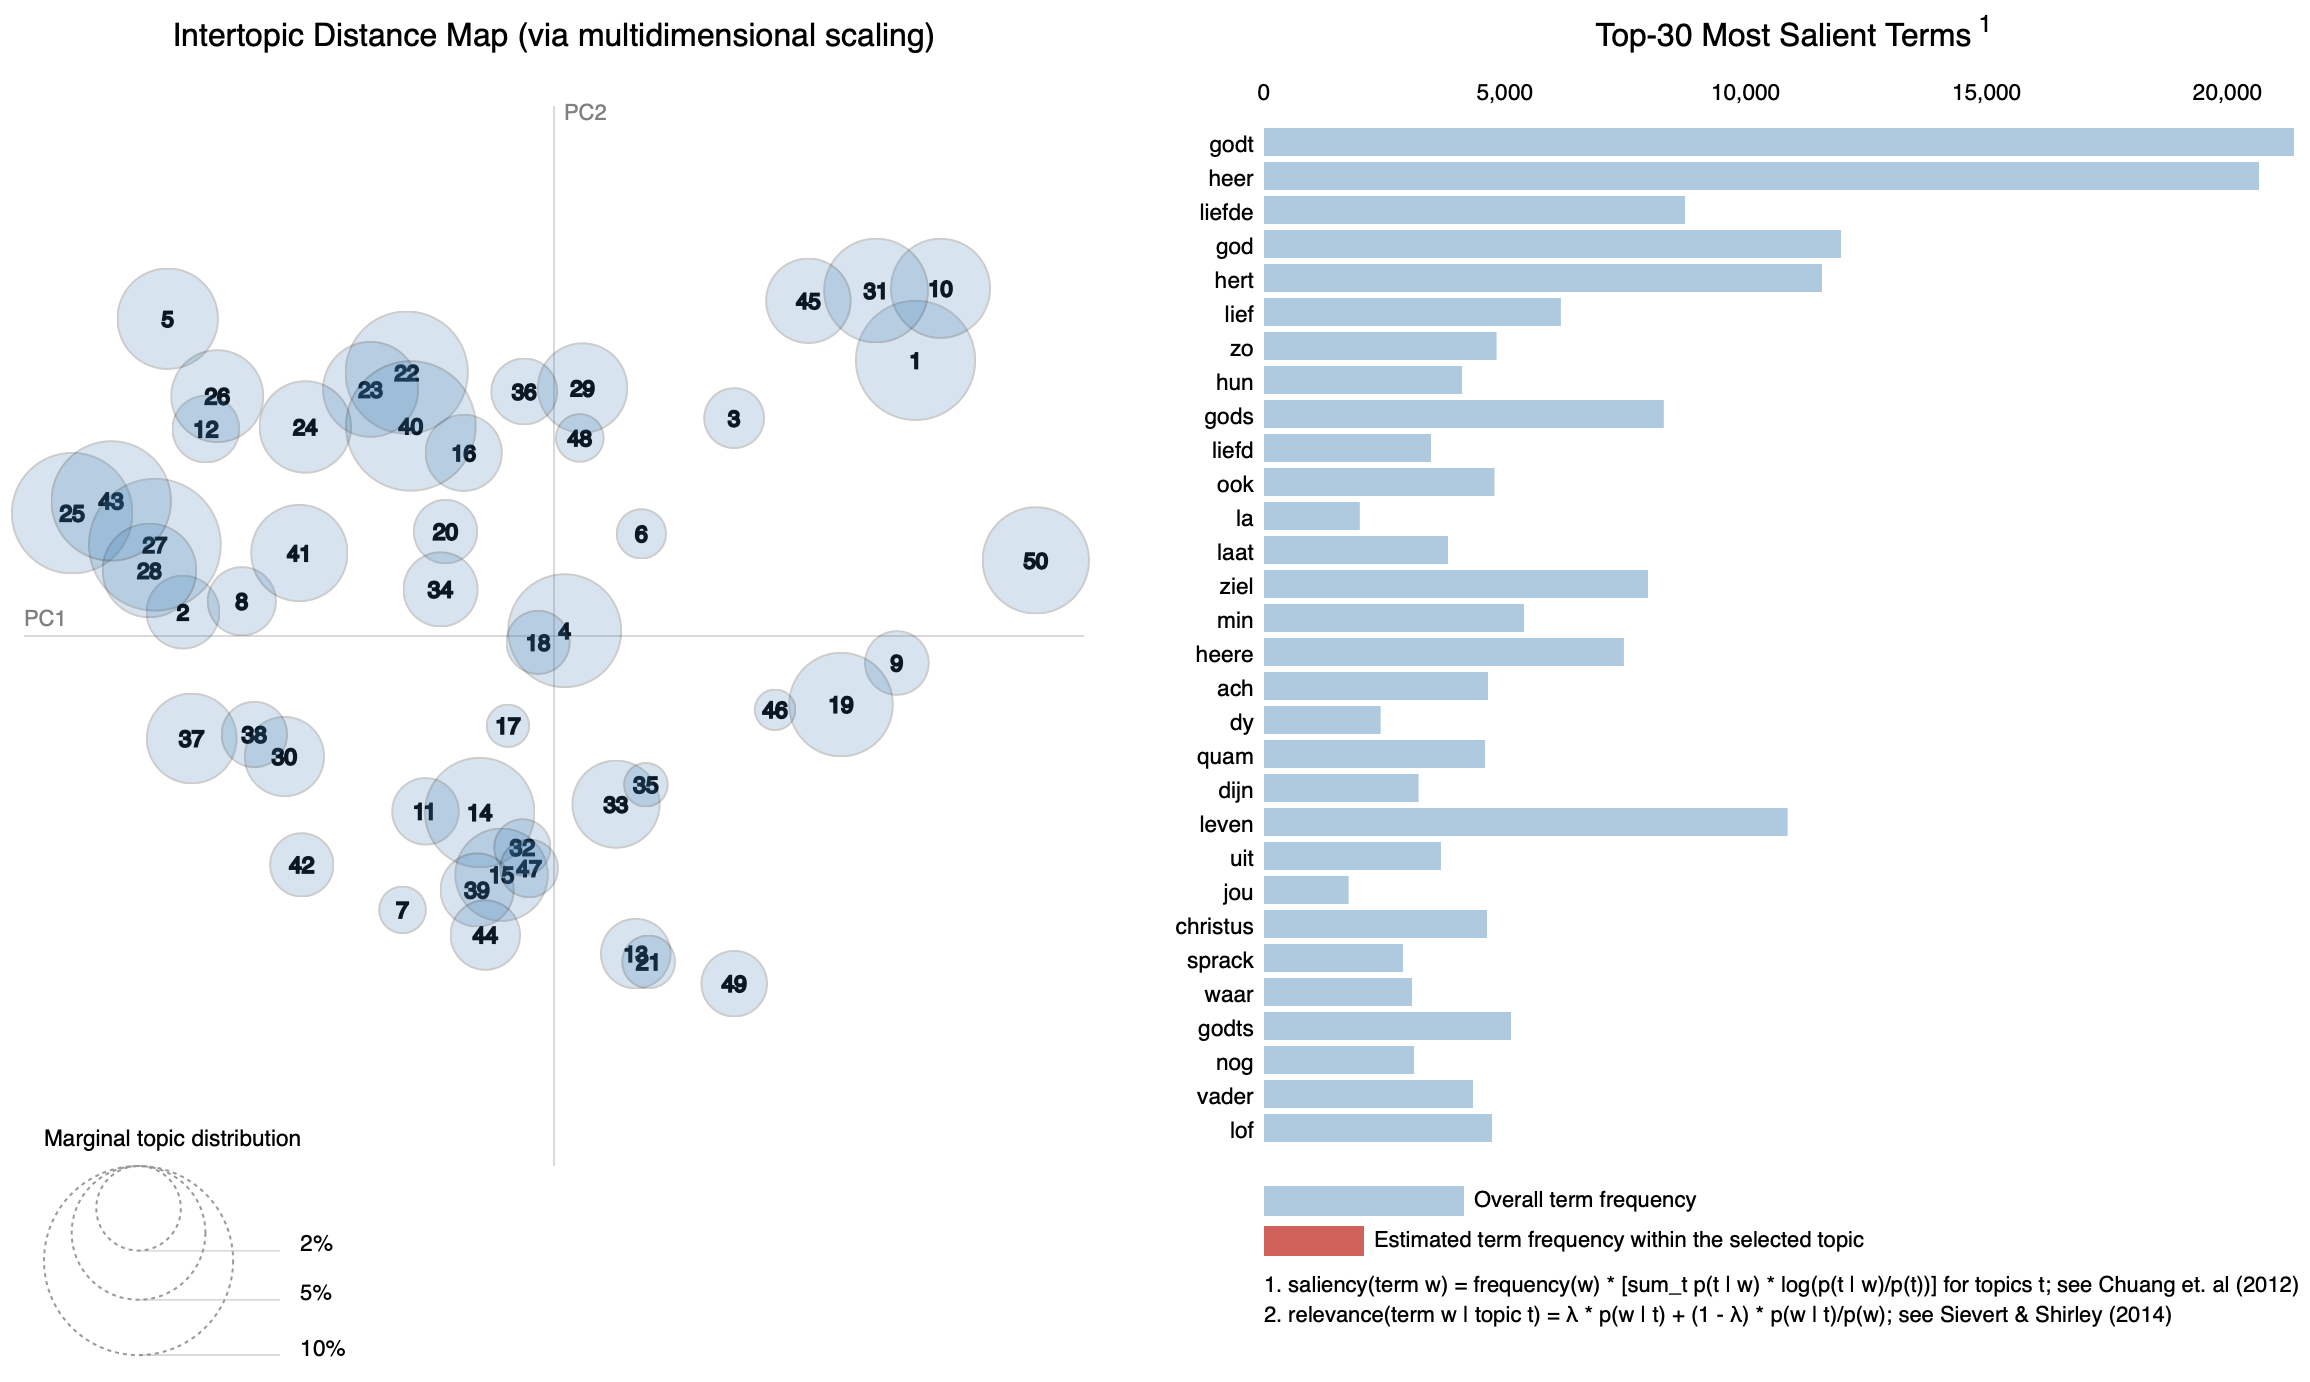
\includegraphics[scale=0.3]{original_pyLDAvis}
	\caption{Visualization of topics in the original corpus with \texttt{pyLDAvis}}
	\label{fig:pyLDAvisOriginal}
\end{figure}

\noindent A good topic model should have bubbles scattered throughout the chart, instead of being clustered in one quadrant. A model with too many topics will typically have many overlapping small sized bubbles clustered in one region of the chart. Although the bubbles in Figure~\ref{fig:pyLDAvisOriginal} are scattered throughout the chart, there are quite a few small sized bubbles, and many of them are overlapping with others. When taking a closer look to the groups with topics, it turns out that the bubbles that cluster together, were also interpreted by me as comparable topics. All bubbles in the top left quadrant are religious topics, as well as some topics in the top right quadrant. When hovering over the most salient terms that are pictured in the right-hand side plot, the topics in which the word in question is represented, are shown. Figure Figure~\ref{fig:pyLDAvisOriginal_godt} confirms the notion that religious topics are clustered in the top left quadrant. The bottom left and right quadrant are filled with the more \enquote{profane} topics, with the two biggest topics on love (49 and 3 or, in Figure~\ref{fig:pyLDAvisOriginal}, 50 and 4) close to the x-axis, as a sort of divider between the two areas. Figure~\ref{fig:pyLDAvisOriginal_liefde} indeed shows that topics on love are scattered throughout the chart, but mainly represented along the x-axis.

\begin{figure}[hbt!]
	\centering
	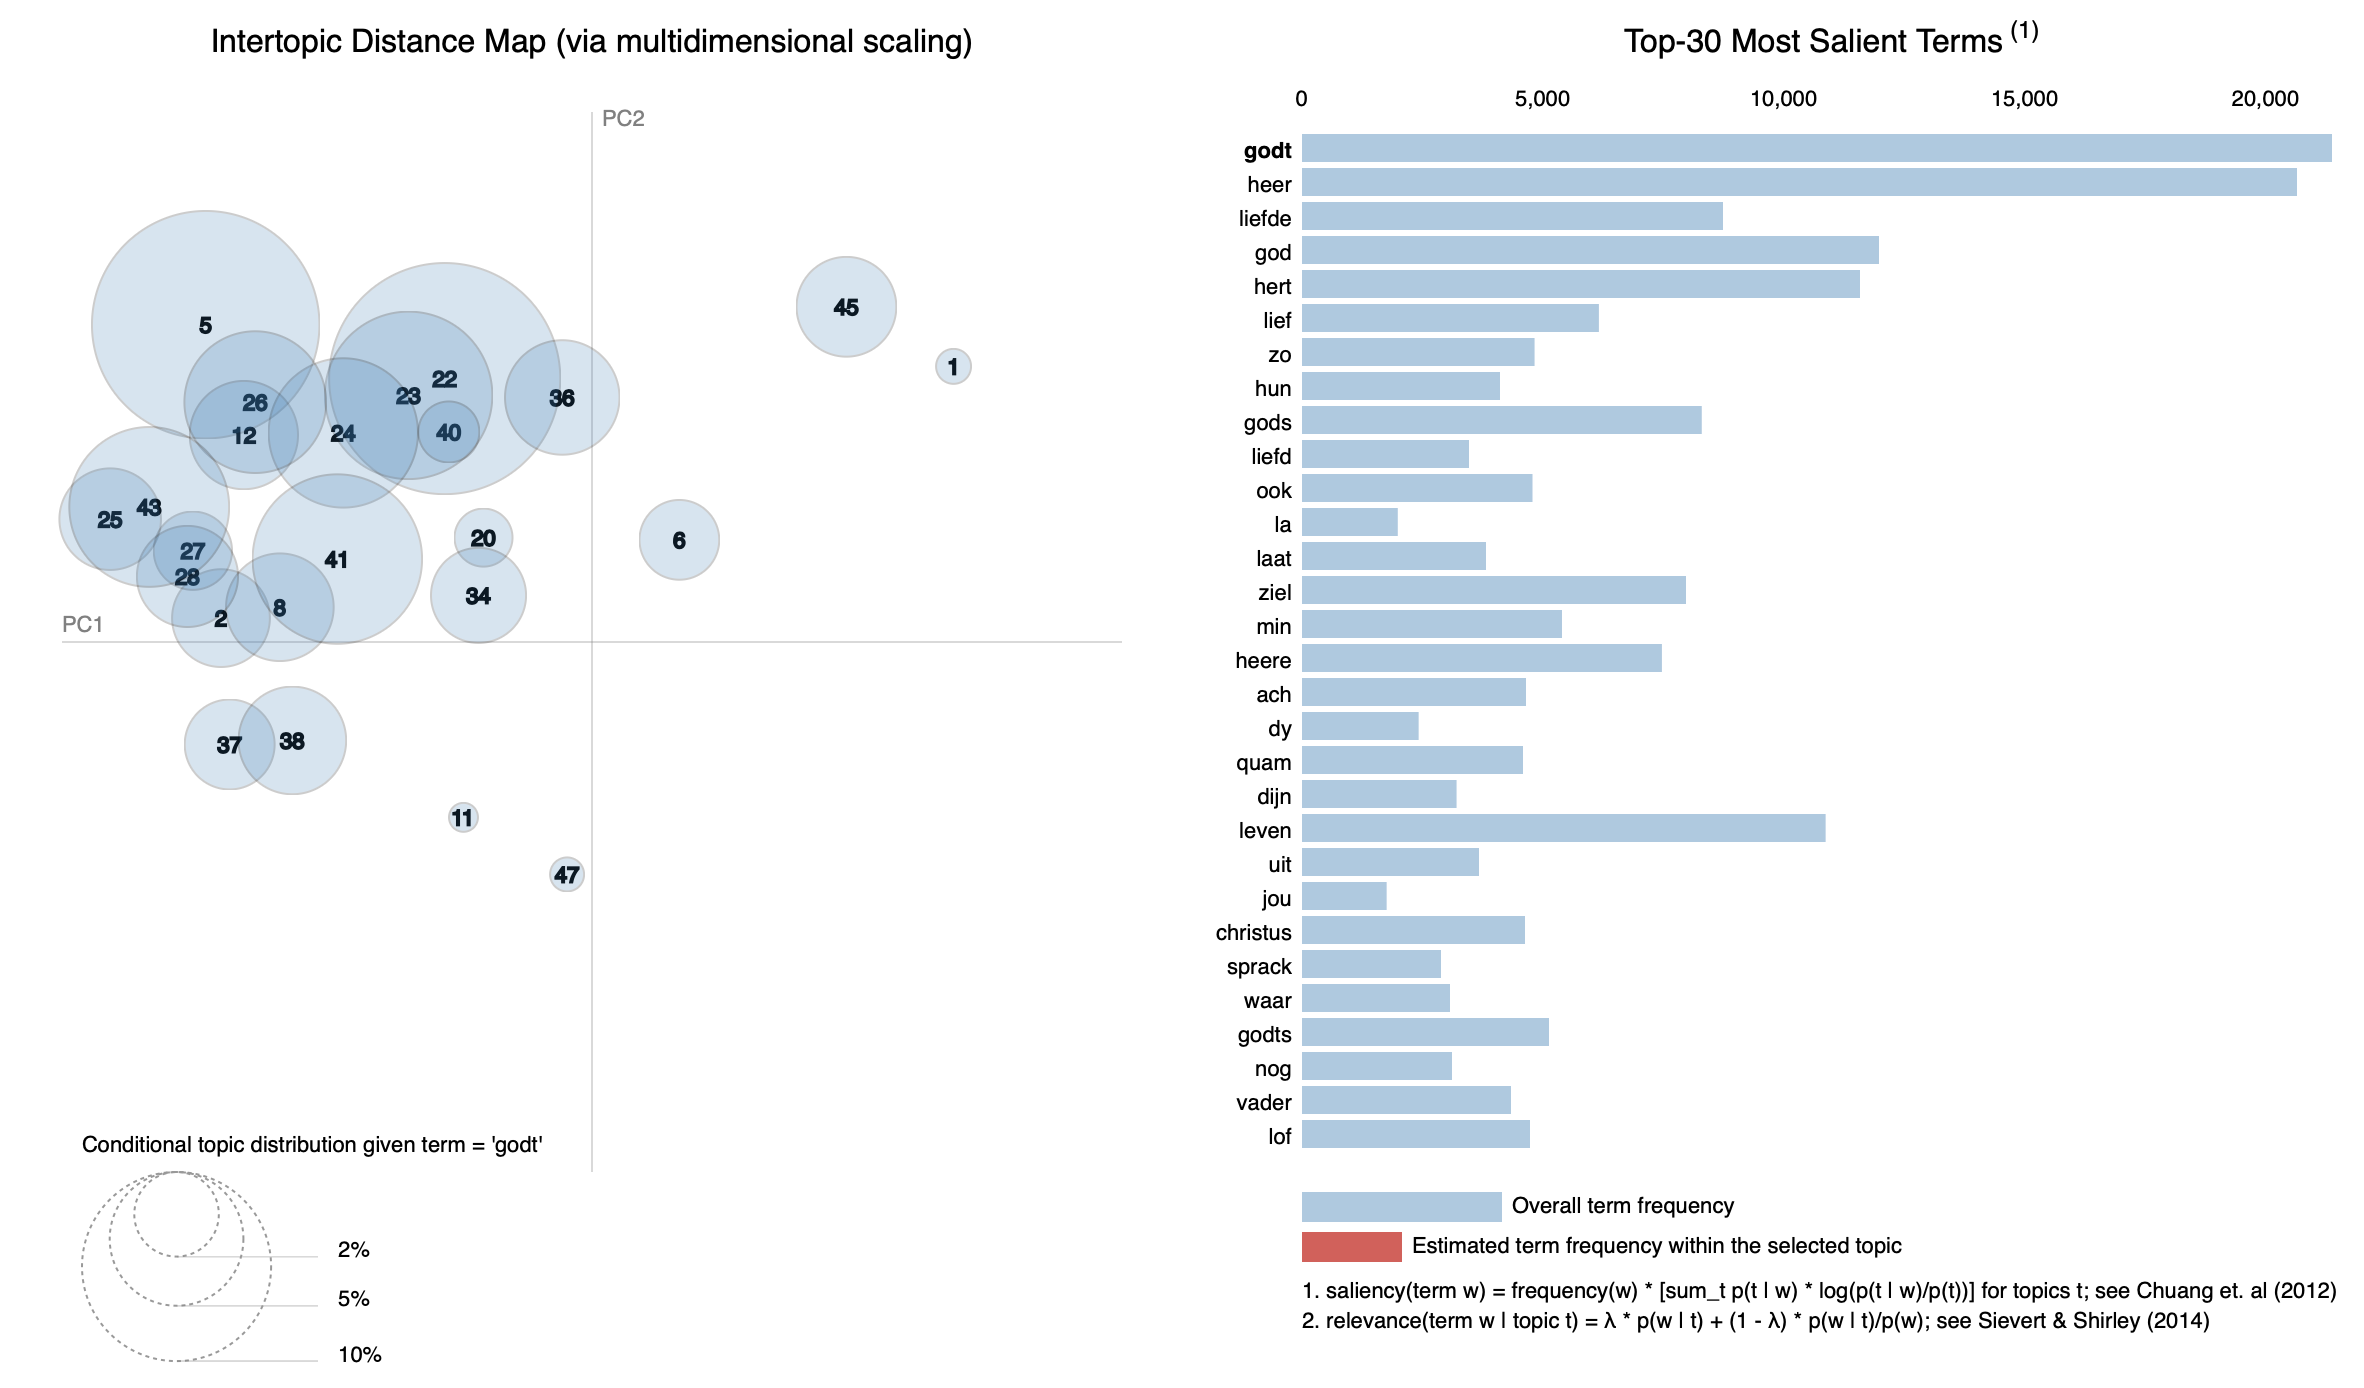
\includegraphics[scale=0.3]{original_pyldavis_godt}
	\caption{Visualization of topics with \textit{godt} in the original corpus}
	\label{fig:pyLDAvisOriginal_godt}
\end{figure}

\begin{figure}[hbt!]
	\centering
	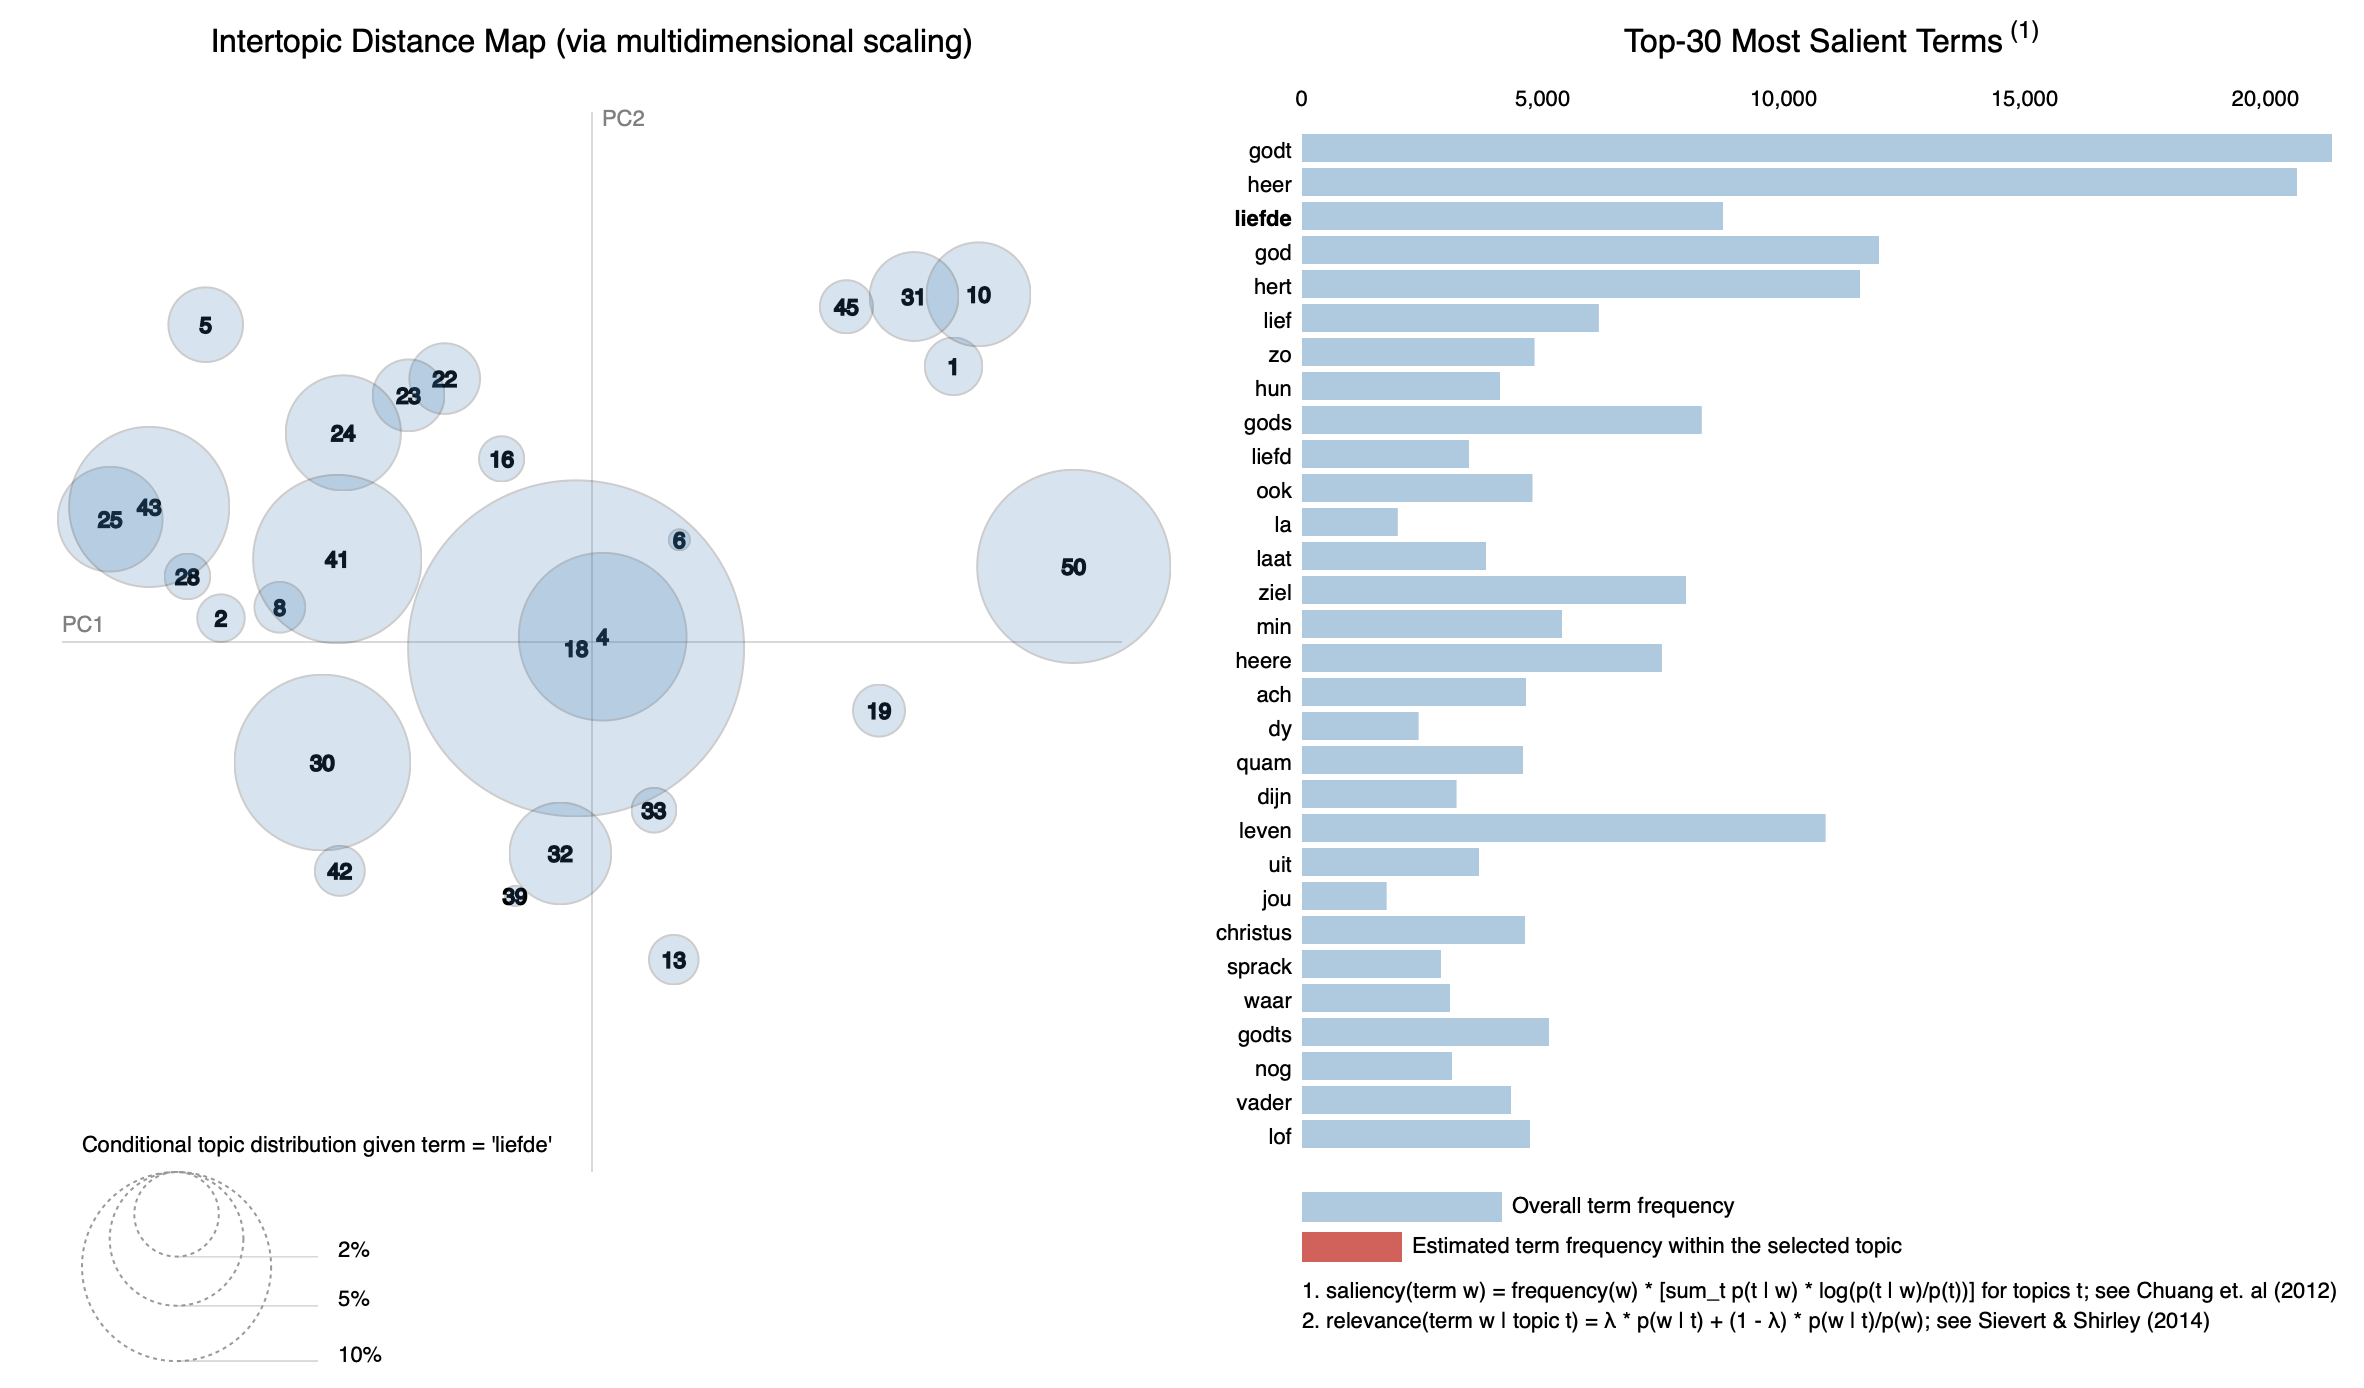
\includegraphics[scale=0.3]{original_pyldavis_liefde}
	\caption{Visualization of topics with \textit{liefde} in the original corpus}
	\label{fig:pyLDAvisOriginal_liefde}
\end{figure}

Since these topics are made from a corpus with unnormalized spelling, there are also topics in which words from a certain time period are clustered, or topics with words that make no sense at all. I shall explain this with a few examples. Topic 47 contains words spelled in a way which was very common in the fifteenth and sixteenth century, such as \enquote{ghoed}, \enquote{dyn}, \enquote{dyne}, \enquote{dyns} and \enquote{dueghd}. To topic 34 I referred as \textit{trash} in Table~\ref{table:DomTopOr}. The words \enquote{dy}, \enquote{yn}, \enquote{soe}, \enquote{uwz} and \enquote{jon} seem to be the result of either a mistake in digitization or tokenization, or a wrong printed lyric. Topic 20 makes clear that there are some songs in the corpus that are written in German or French: there is no other explanation for words such as \enquote{ich}, \enquote{das}, \enquote{je} and \enquote{vous} clustered together. Normalization of the spelling would not solve the problem of foreign songs, but it can reduce the number of topics that are built based on the time-specific spelling of the words that are in it. In the next paragraph I therefore built a topic model from the INL-normalized corpus, to see if this model outstands the one built and discussed in the current paragraph.

\subsection{INL-normalized corpus}
The dictionary that was build from the INL-normalized corpus, contained at first 186,692 unique tokens. The setting \texttt{no\_below = 2} resulted in the elimination of 114,100 tokens (the words with a value of \texttt{1} in the dictionary). The number of remaining tokens was 72,592. That is already 17,000 less words than in the dictionary of the original corpus. Again, I build a model with 50 topics. The coherence score of this model is 0.4683, which is lower than the coherence score from the previous built model. Again, I tried to assign a subject to each topic. Besides that, I investigated also which topic is the dominant for each song, and grouped the dominant topics to count how many times they appear. The results of both actions are stored in Table~\ref{table:DomTopINL}.

While assigning subjects to the topics that were composed from the INL-normalized corpus, I noticed that this time, when compared to the topics composed from the original corpus, much more topics were inconclusive and therefore hard to assign a subject to. Topic 38 and topic 15 for example are in the Top10 most dominant topics, but their subject is almost impossible to distill (see Figures~\ref{fig:Topic38INL} and~\ref{fig:Topic15INL}). The word \enquote{zek}, prominent in topic 15, I already discussed earlier, when pointing out to wrong spelling corrections that were performed by the INL-tool. In the example from Chapter 5, the word \enquote{zig} was normalized to \enquote{zek}. It is possible though, that other words, resembling \enquote{zig}, were also normalized to \enquote{zek}. The same applies to the word \textit{scene} in topic 38. The suspicion prevails that this is also the result of a wrong normalization, since there is no early modern Dutch resembling equivalent for \enquote{scene}. The problem is, though, that there is no actual proof of that. The INL-tool does not give any statistical output containing data on which normalizations were performed on which words. This fact makes that I am going to question the results from the INL-normalized corpus more and more: how do I know that the words that are clustered in these topics still contain the same meaning as they supposed to contain?

\begin{figure}
	\begin{minipage}[c]{0.48\linewidth}
		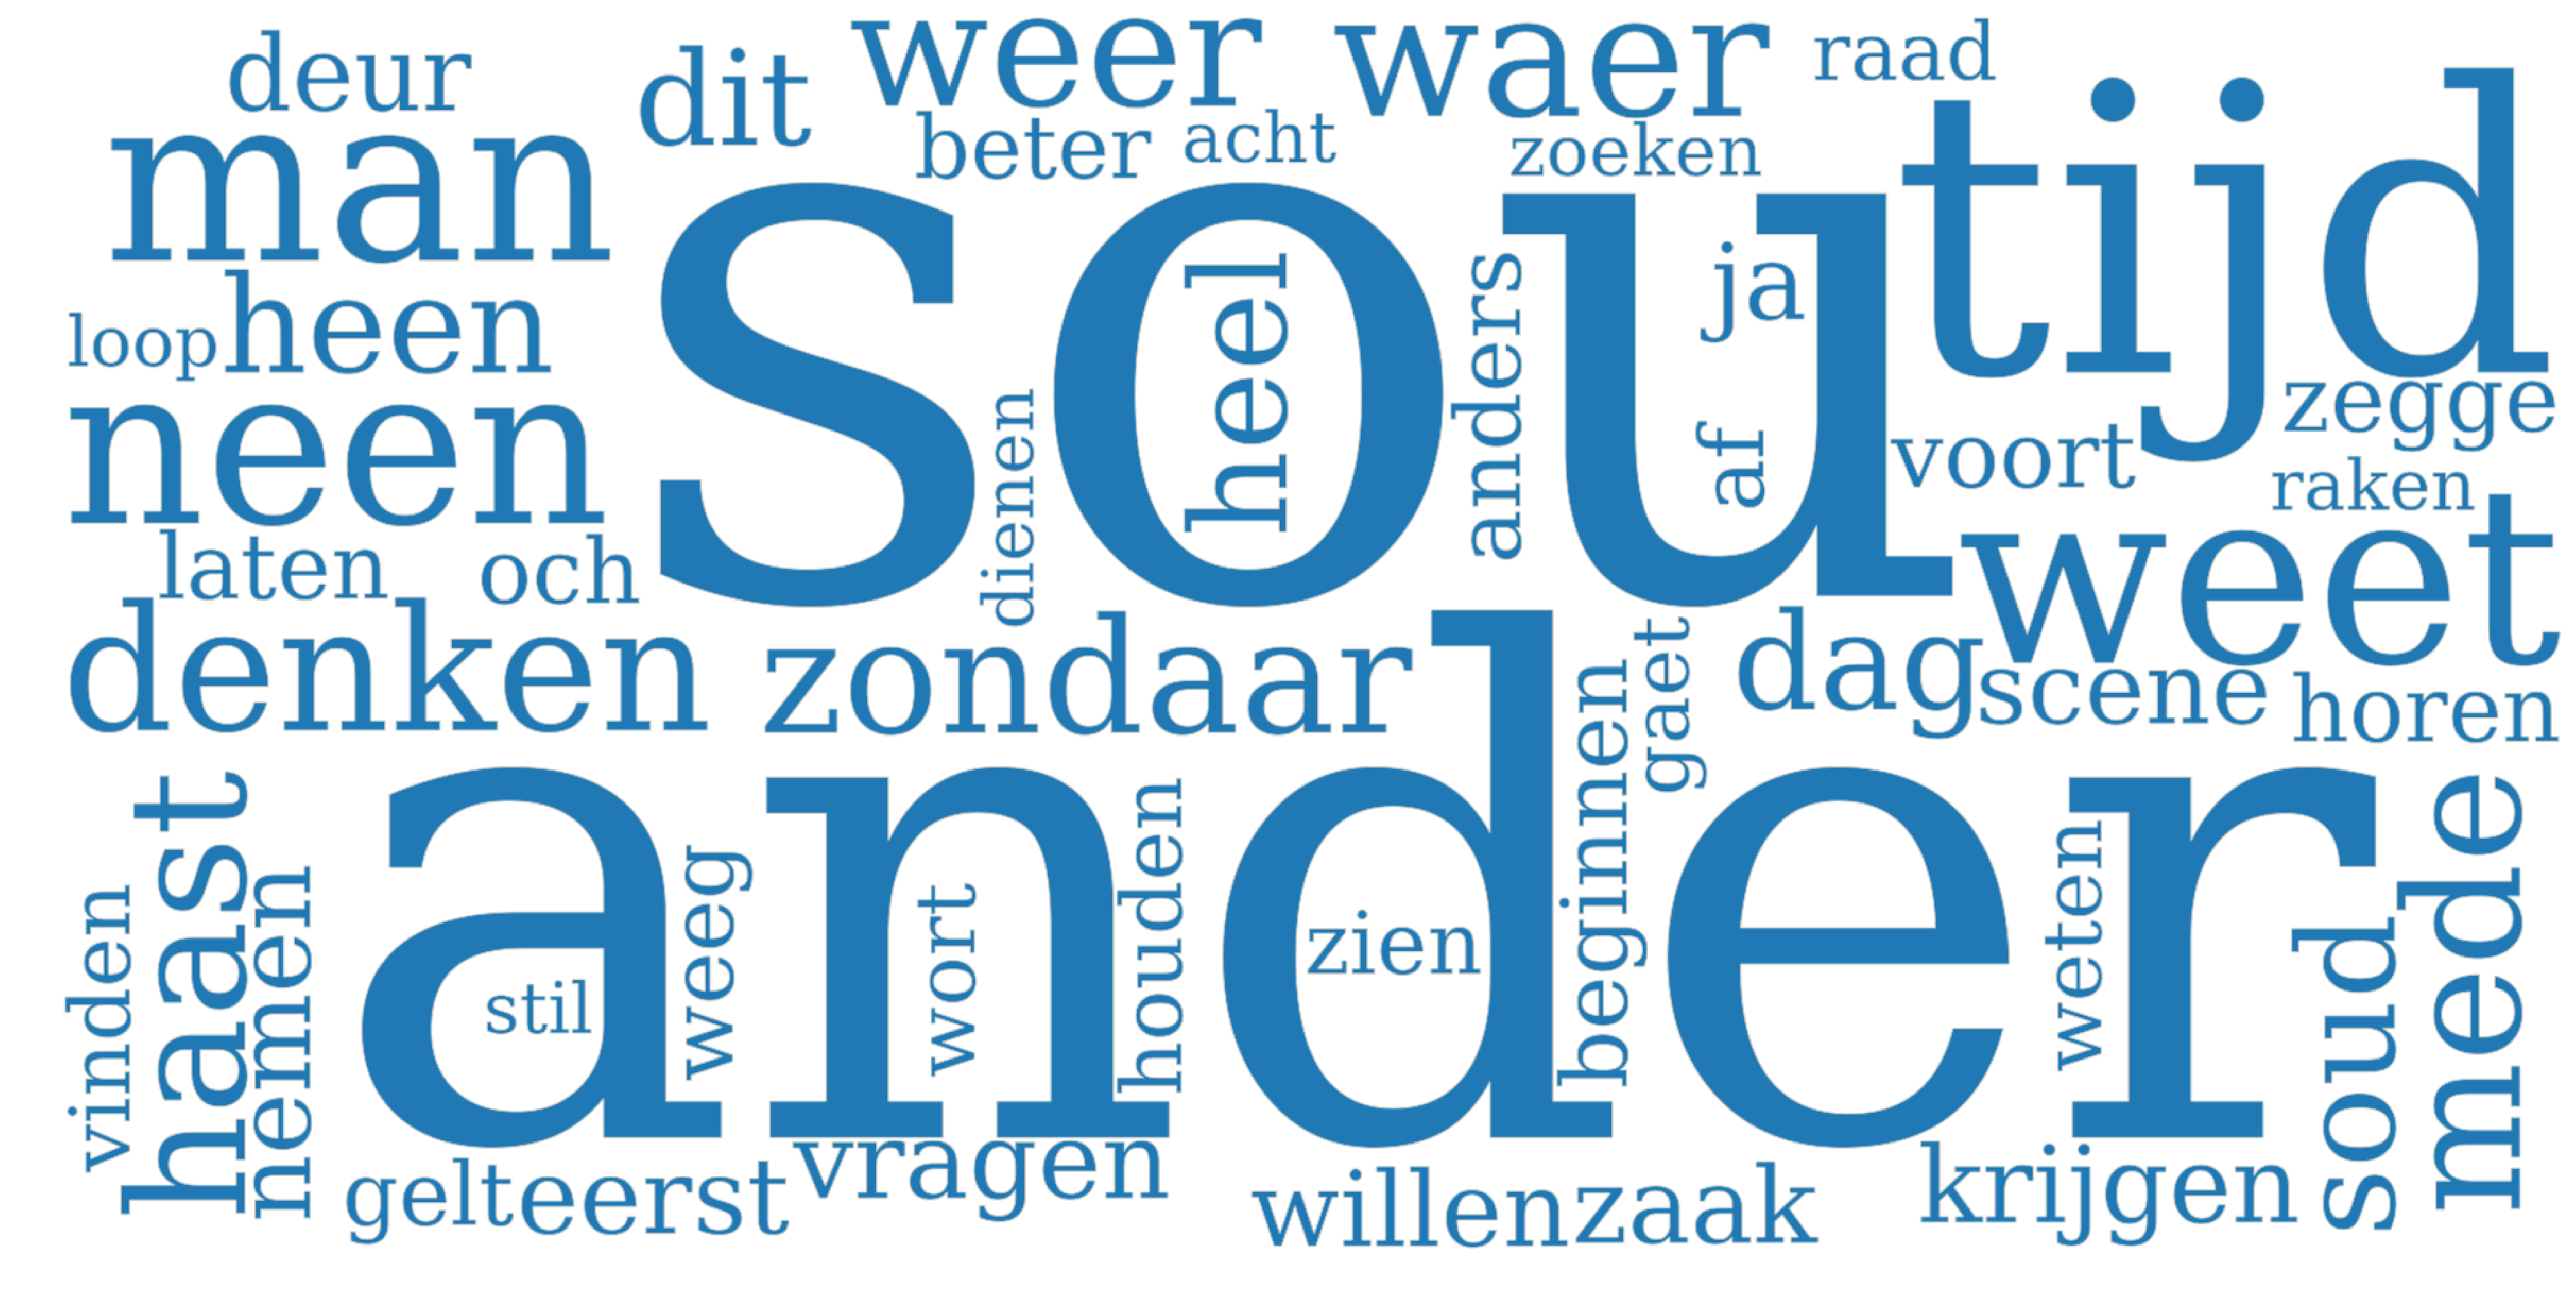
\includegraphics[width=\linewidth]{INL_topic38}
		\caption{\textit{???} (38, INL)}
		\label{fig:Topic38INL}
		\vspace{4ex}
	\end{minipage}%%
	\begin{minipage}[c]{0.48\linewidth}
		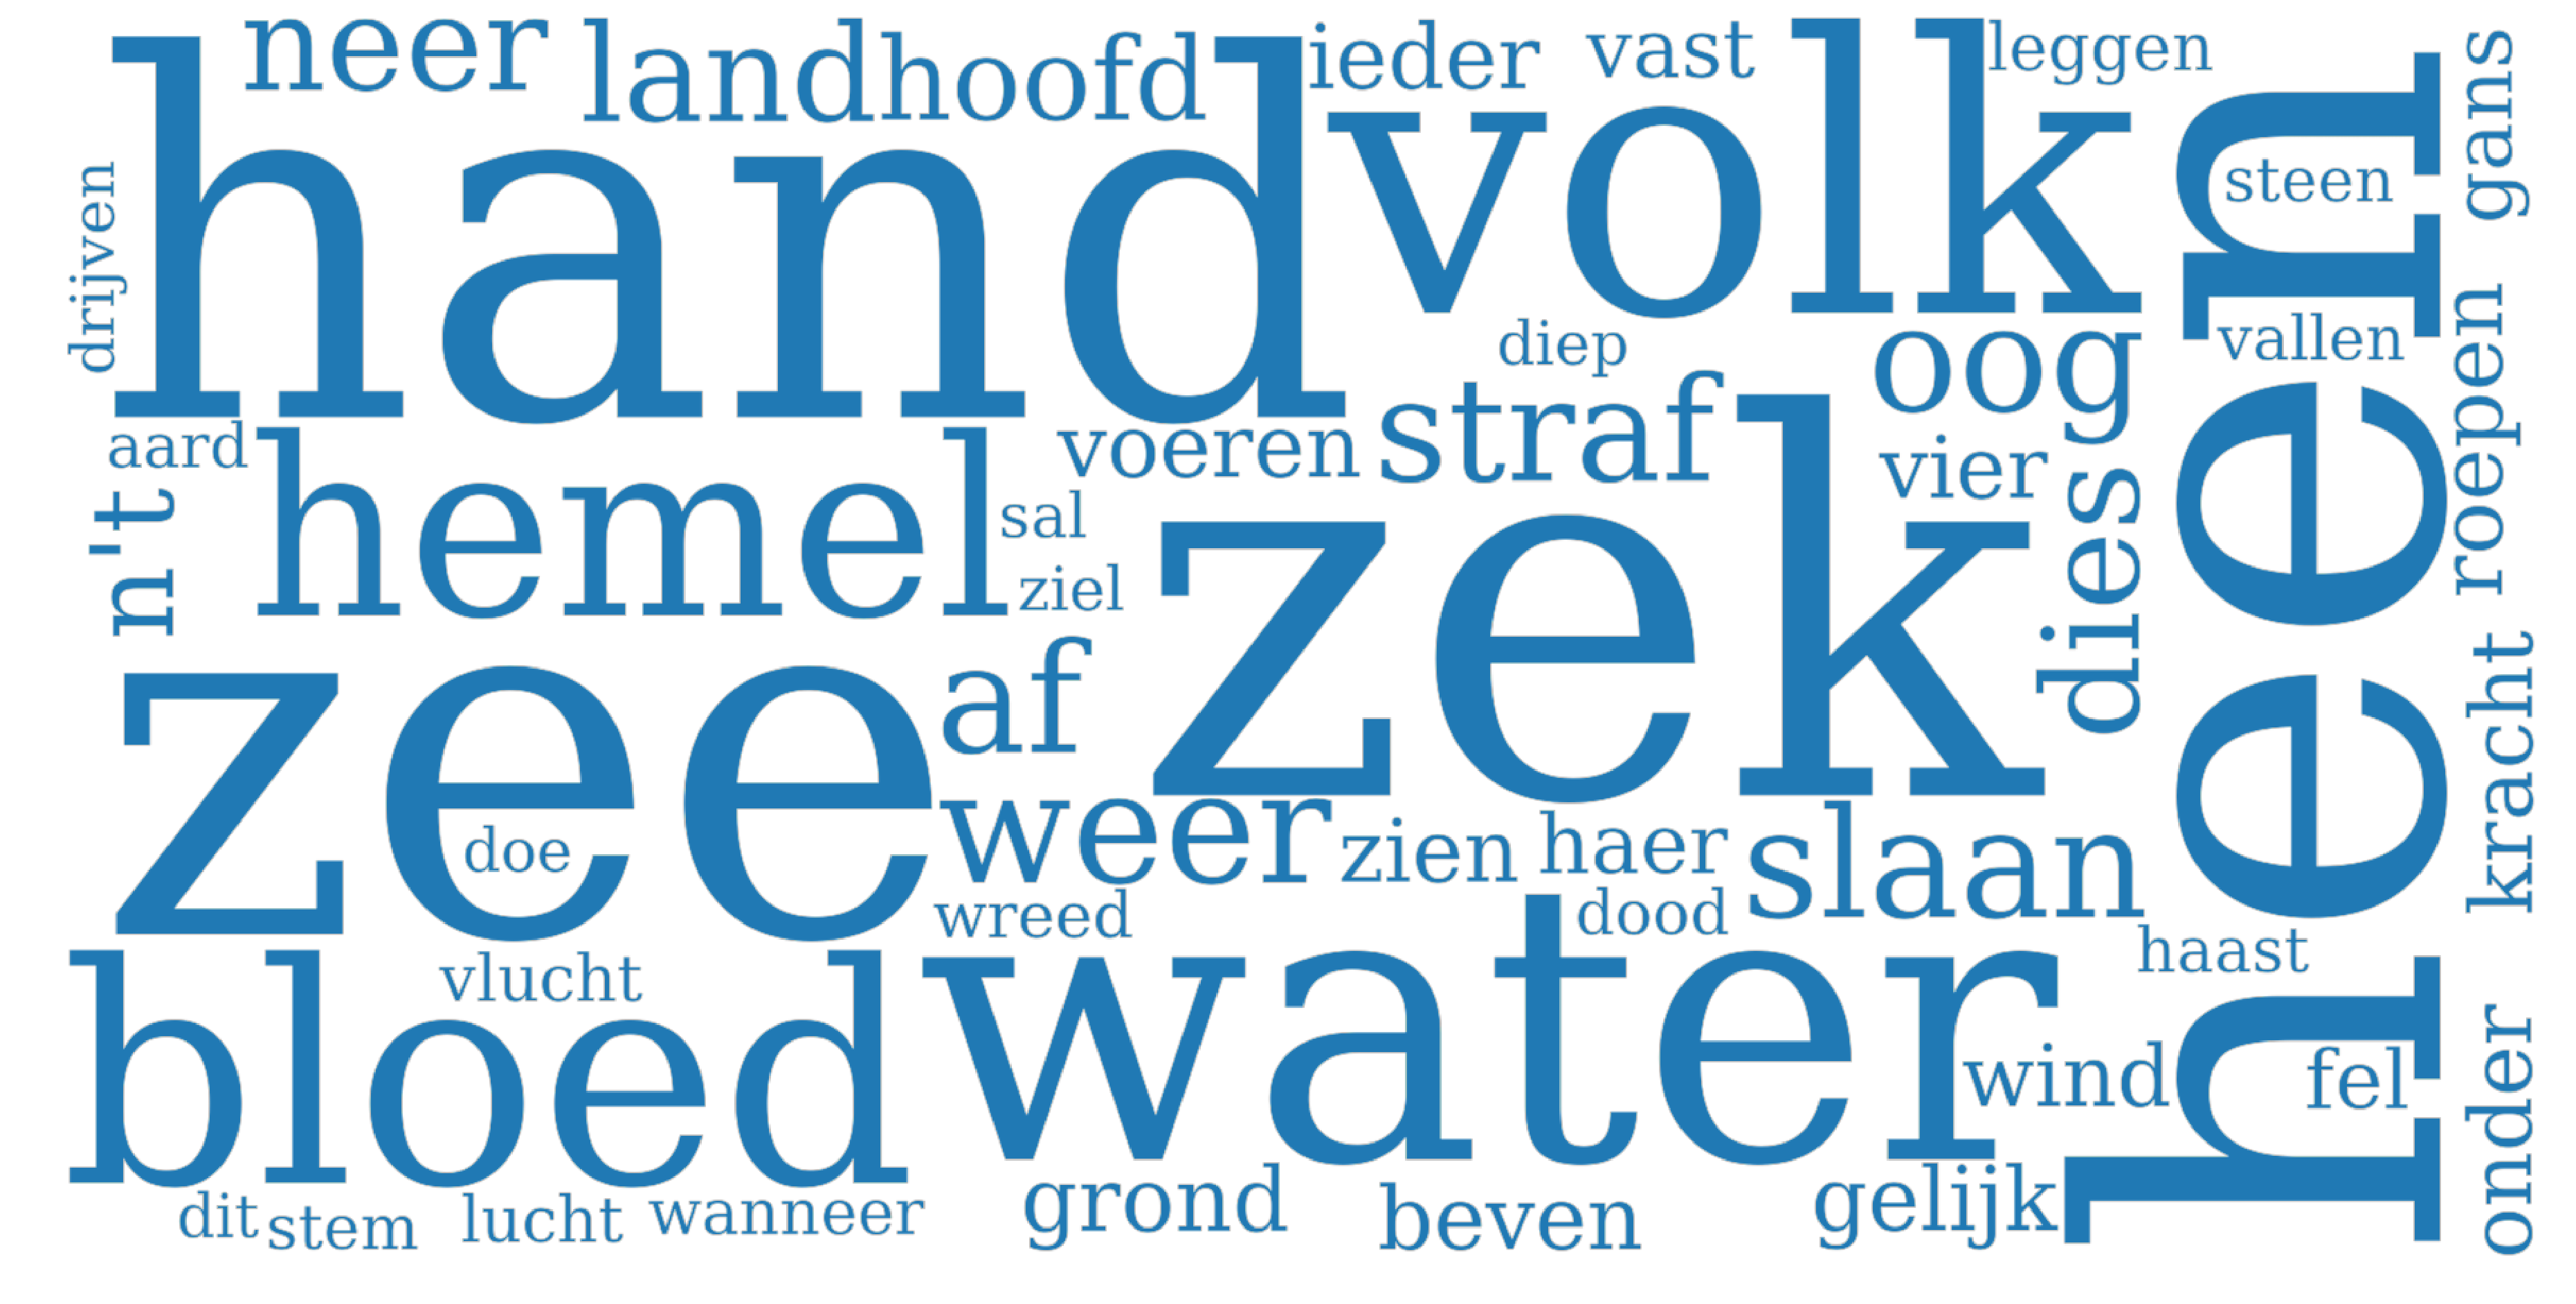
\includegraphics[width=\linewidth]{INL_topic15}
		\caption{\textit{???} (15, INL)}
		\label{fig:Topic15INL}
		\vspace{4ex}
	\end{minipage}%%
\end{figure}

\begin{table}
	\begin{minipage}{0.5\textwidth}
		\begin{tabular}{ccl}
			\toprule
			Topic & Songs & Subject \\
			\midrule
			24             &  1337 & sadness  \\
			39             &  1113 & heart \& soul \\
			21             &   965 & religion \& Christ \\
			4              &   952 & man \& life \\
			25             &   910 & live \& love \\
			38             &   903 & ??? \\
			16             &   862 & religion \\
			26             &   859 & love \\
			33             &   807 & religion \\
			15             &   759 & ??? \\
			30             &   671 & religion \& happiness \\
			42             &   663 & religion \& passion \\
			37             &   576 & physical love \\
			20             &   550 & bucolic songs \\
			22             &   510 & religion \& love \\
			2              &   496 & family??? \\
			11             &   492 & persons \\
			34             &   462 & religion \\
			6              &   459 &  drinking \\
			9              &   452 & live \& die \\
			3              &   430 & religion \\
			8              &   425 & religion \\
			41             &   407 & Christmas \\
			43             &   394 & marriage \\
			29             &   369 & religion \\
			\vdots & \vdots & \vdots \\
			\bottomrule
		\end{tabular}
	\end{minipage} \hfill
	\begin{minipage}{0.5\textwidth}
		\begin{tabular}{|ccl}
			\toprule
			Topic & Songs & Subject  \\
			\midrule
			\vdots & \vdots & \vdots \\
			10             &   354 & beauty??? \\
			28             &   351 & old spelling \\
			40             &   332 & religion \& passion \\
			47             &   330 & religion \\
			45             &   316 & love  \\
			5              &   267 &  truth \& lie \\
			49             &   260 & nature \\
			23             &   256 & religion \& positive emotions \\
			19             &   252 & ??? \\
			32             &   249 & sea \\
			18             &   246 & mother \& father \\
			14             &   241 & nation \& country \\
			13             &   230 & church \\
			17             &   224 & religion \\
			48             &   218 & enemy \\
			7              &   211 & Old Testament \\
			27             &   176 & happiness \& singing \\
			46             &   156 & sun \\
			0              &   147 & eternal life \\
			31             &   144 & French \\
			44             &   128 & mythology \\
			1              &   121 & possessives \\
			12             &   113 & German \\
			36             &    94 & trash \\
			35             &    58 & solfège \\
			\bottomrule
		\end{tabular}
	\end{minipage}
\caption{Dominant topics in INL-normalized corpus (\textit{n} = 22,297)}
\label{table:DomTopINL}
\end{table}

A visualization with \texttt{pyLDAvis} actually confirms these doubts. Figure~\ref{fig:pyLDAvisINL} shows that, instead of an improved scatter plot compared to Figure~\ref{fig:pyLDAvisOriginal}, the topics overlap just as much. It even seems that the bubbles, except the four in the bottom right quadrant, are clustered closer to each other. This also explains the difficulty to assign a specific subject to many topics. I can therefore conclude that a normalization tool as raw and straightforward as the INL-tool does not improve further results of textual analysis. The third option is building topics from the corpus that is normalized with the VARD2-tool.

\begin{figure}[hbt!]
	\centering
	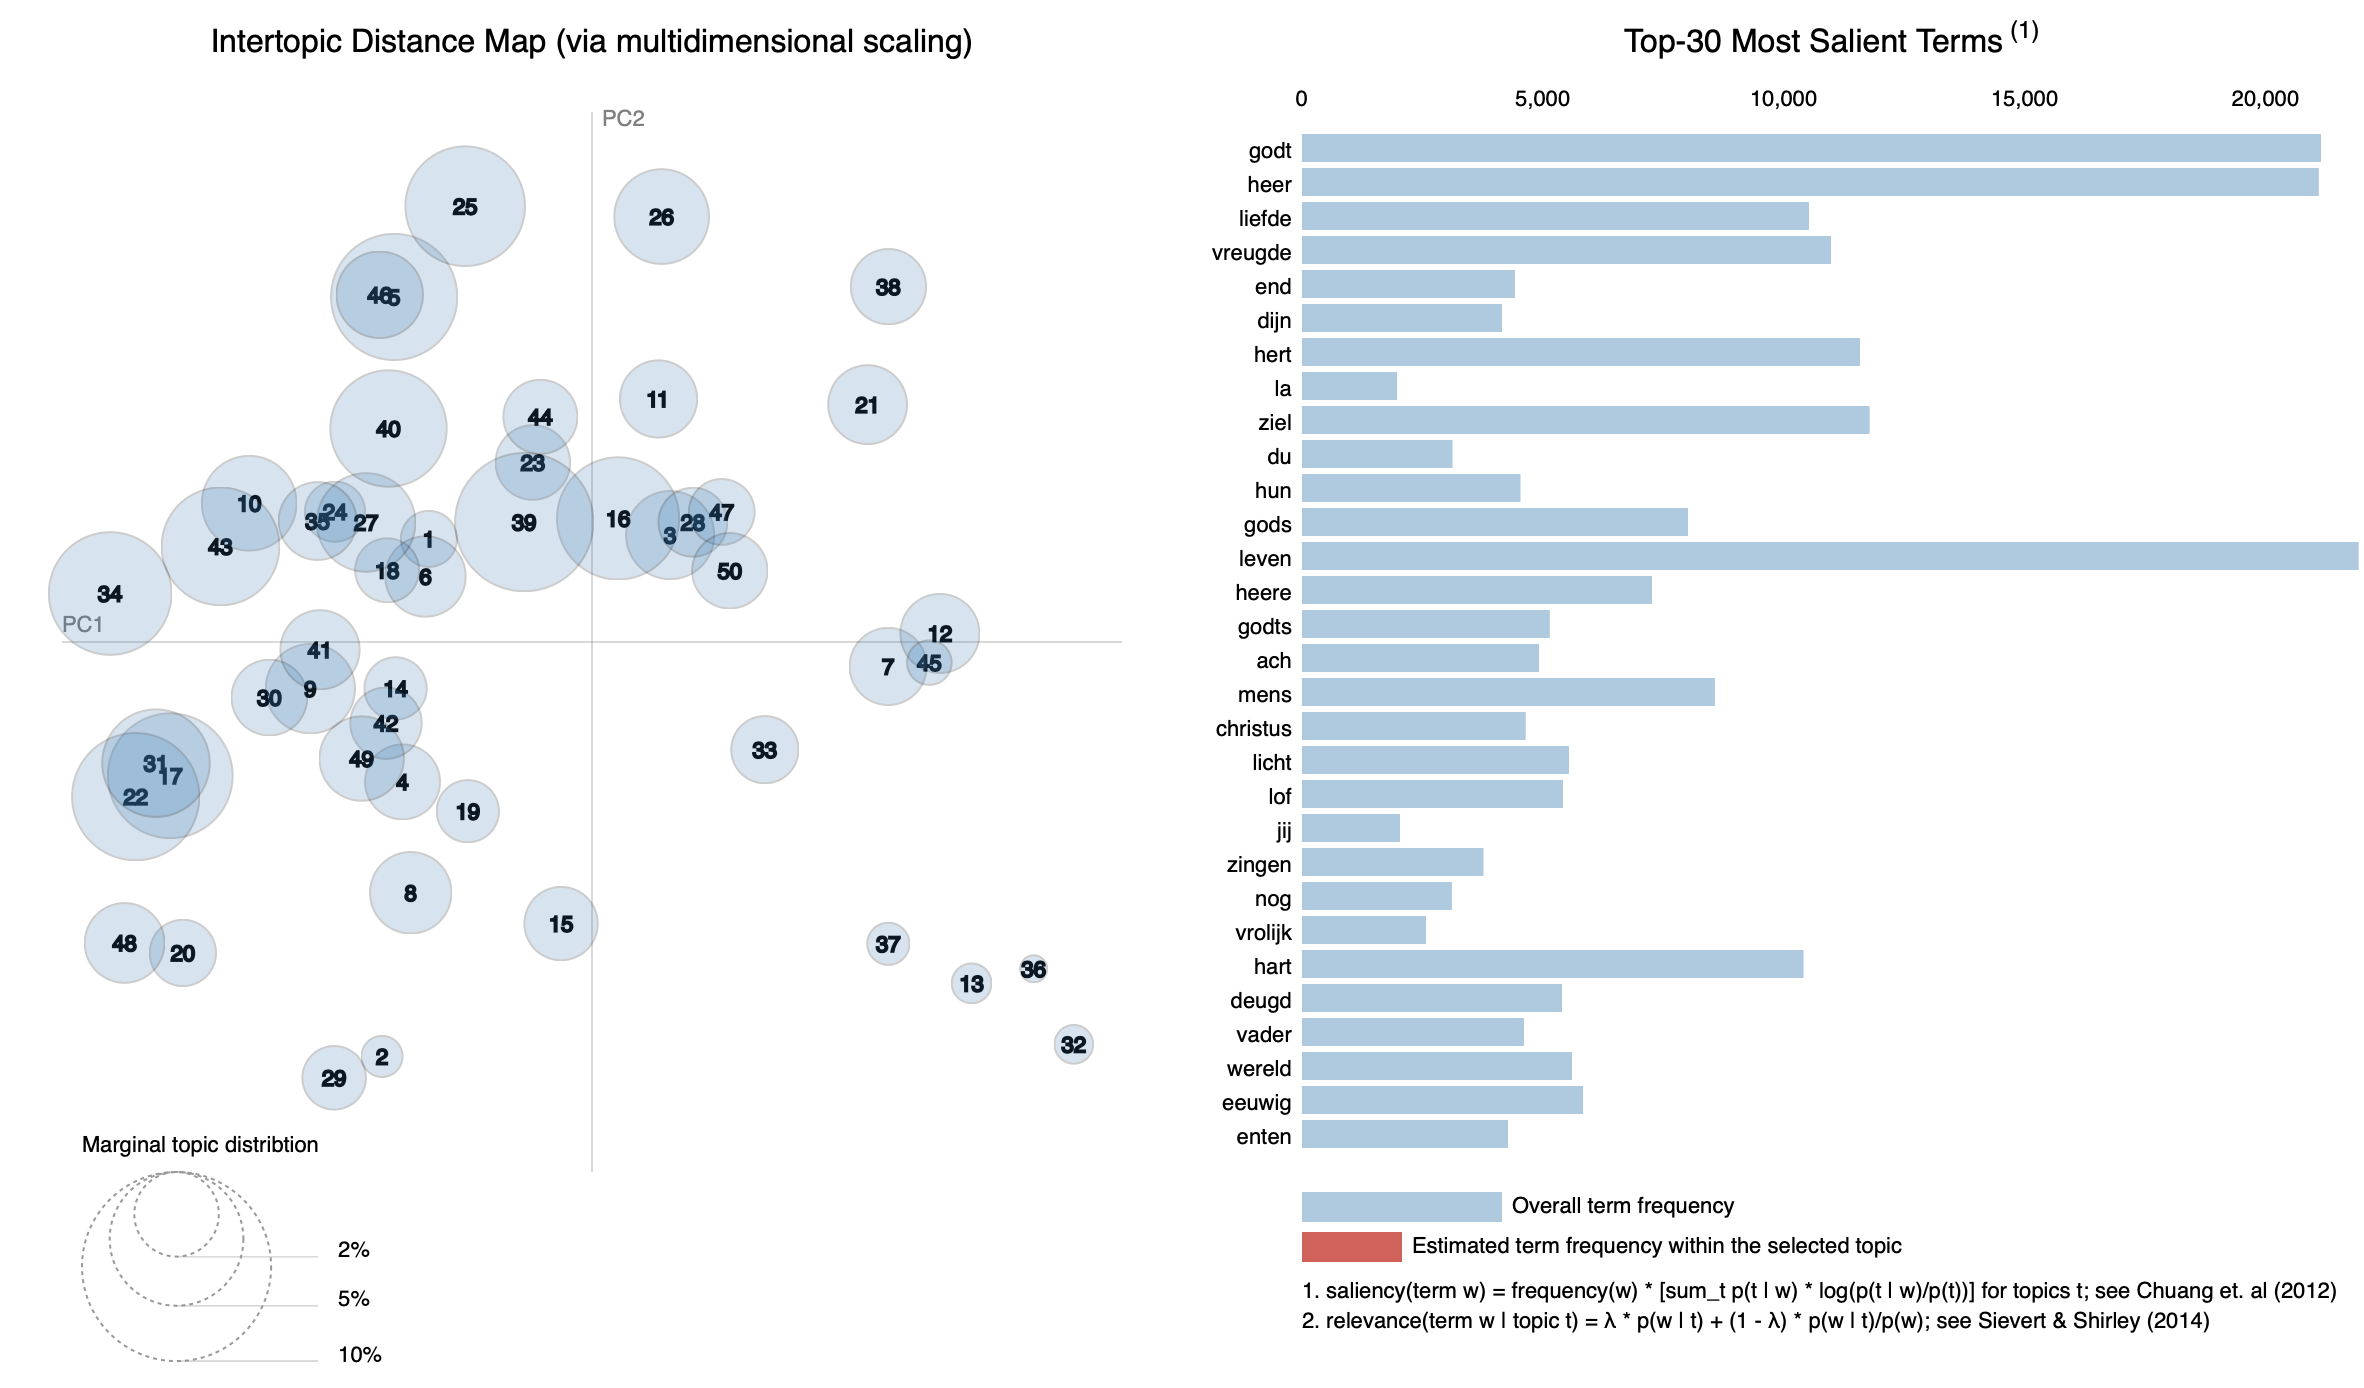
\includegraphics[scale=0.3]{INL_pyLDAvis}
	\caption{Visualization of topics in the INL-normalized corpus with \texttt{pyLDAvis}}
	\label{fig:pyLDAvisINL}
\end{figure}

\subsection{VARD2-normalized corpus}
At first there were 194,159 tokens in the dictionary that was built from the VARD2-normalized corpus. After eliminating 117,045 tokens with \texttt{no\_below = 2}, 77,114 tokens remained. For the final time I let the tool compose 50 topics. The coherence score of the built model was 0.4962, which is higher than the score of the model built from the INL-normalized corpus. The visualization made with \texttt{pyLDAvis} immediately shows that this topic model obtained better results than the one built in the previous paragraph. The bubbles are more evenly scattered throughout the chart, and less bubbles overlap with each other. This creates the expectation that the subjects of the topics made from this version of the corpus, are easier to assign. Below I discuss some topics and how I assigned a subject to them. The results are stored in Table~\ref{table:DomTopVARD2}. Besides, I examined for each topic which song represented this topic at best, in other words, which song had the highest contribution to that specific topic, using the following code: 

\begin{lstlisting}
song_topic_highest_contribution = pd.DataFrame()
song_topics_outdf_grpd = dominant_topics.groupby("dominant_topic")

for i, grp in song_topics_outdf_grpd:
song_topic_highest_contribution = pd.concat([song_topic_highest_contribution, grp.sort_values(["perc_contribution"], ascending=[0]).head(1)], axis=0)

song_topic_highest_contribution.reset_index(drop=True, inplace=True)
song_topic_highest_contribution.columns = ["id", "topic", "perc_contribution"]
\end{lstlisting}

To topic 28 (Figure~\ref{fig:topic28VARD2}), the most prevalent topic in this corpus, I assigned the topic \textit{religion \& intangibility}, since the words in this topic were mainly about the intangible aspects of religion, such as \enquote{ziel}, \enquote{geest} and \enquote{eeuwig}. The song that represents this topic the most, is a sung version of the Lord's prayer (\texttt{id} = 118423), of which I quote the first three stanzas below:

\begin{quote}
	 ONse Vader in Hemelrijck,\\
	Die ons heet kinders al gelijck,\\
	En wilt dat wy u roepen aen,\\
	Als wy met node zijn bevaen:\\
	Geeft dat niet bidt alleen den mondt,\\
	Maer dat het gae uyt 's herten gront.\\
	
	Geheyligt uwen name zy,\\
	U woordt ongevalscht blijv' ons by:\\
	Dat wy oock leven heyliglijck,\\
	Na uwen name weerdiglijck,\\
	Behoet ons Heer, voor valsche leer,\\
	Dat 't arm vervoerde volck bekeer.\\
	
	U Koninghrijck koom', Heere goet,\\
	Hier en hier na. Den trooster soet\\
	Geeft ons dien Chrisius ons toesey\\
	Met zijn gaven menigerley:\\
	Breeckt Satans tooren ende macht;\\
	Voor zijn ergheyt u Kercke wacht.
\end{quote}

\noindent It is understandable that this particular song represents this topic: the Lord's Prayer commemorates specifically the intangible aspects of the christian belief. Topic 27 (Figure~\ref{fig:topic27VARD2}), to which I assigned \textit{world \& money}, is represented at best by this song, dated from 1645 (\texttt{id} = 3207):

\begin{quote}
	ACh! snoode overdaedt,\\
	Vrouw-voedtster van de vuyle dartelheyt,\\
	Oorsaeck van alle quaedt,\\
	Of immers 't geen den wegh daer toe bereyt:\\
	V weelde baert veel onghemack,\\
	En Wellust is een lastigh pack.\\
	
	Die stil en wel te vre'en\\
	Met redelijck behoef is wel vernoegh,\\
	En gaet in vrede heen,\\
	En is gherust hoe 't Godt de Heere voeght:\\
	Die isser vry veel beter an;\\
	Ghenoegh, dat maeckt een deftigh man.\\
	
	Ghnoegh heeft overvloedt,\\
	Schoon dat sen kasjes ledigh zijn van geldt;\\
	Ghenoegh heeft schat en goedt,\\
	Ghenoegh is nimmermeer om Goudt ontsteldt:\\
	Hy leeft gherust die wynigh heeft,\\
	En by sijn weynigh eerlijck leeft.
\end{quote}

\begin{figure}[hbt!]
	\centering
	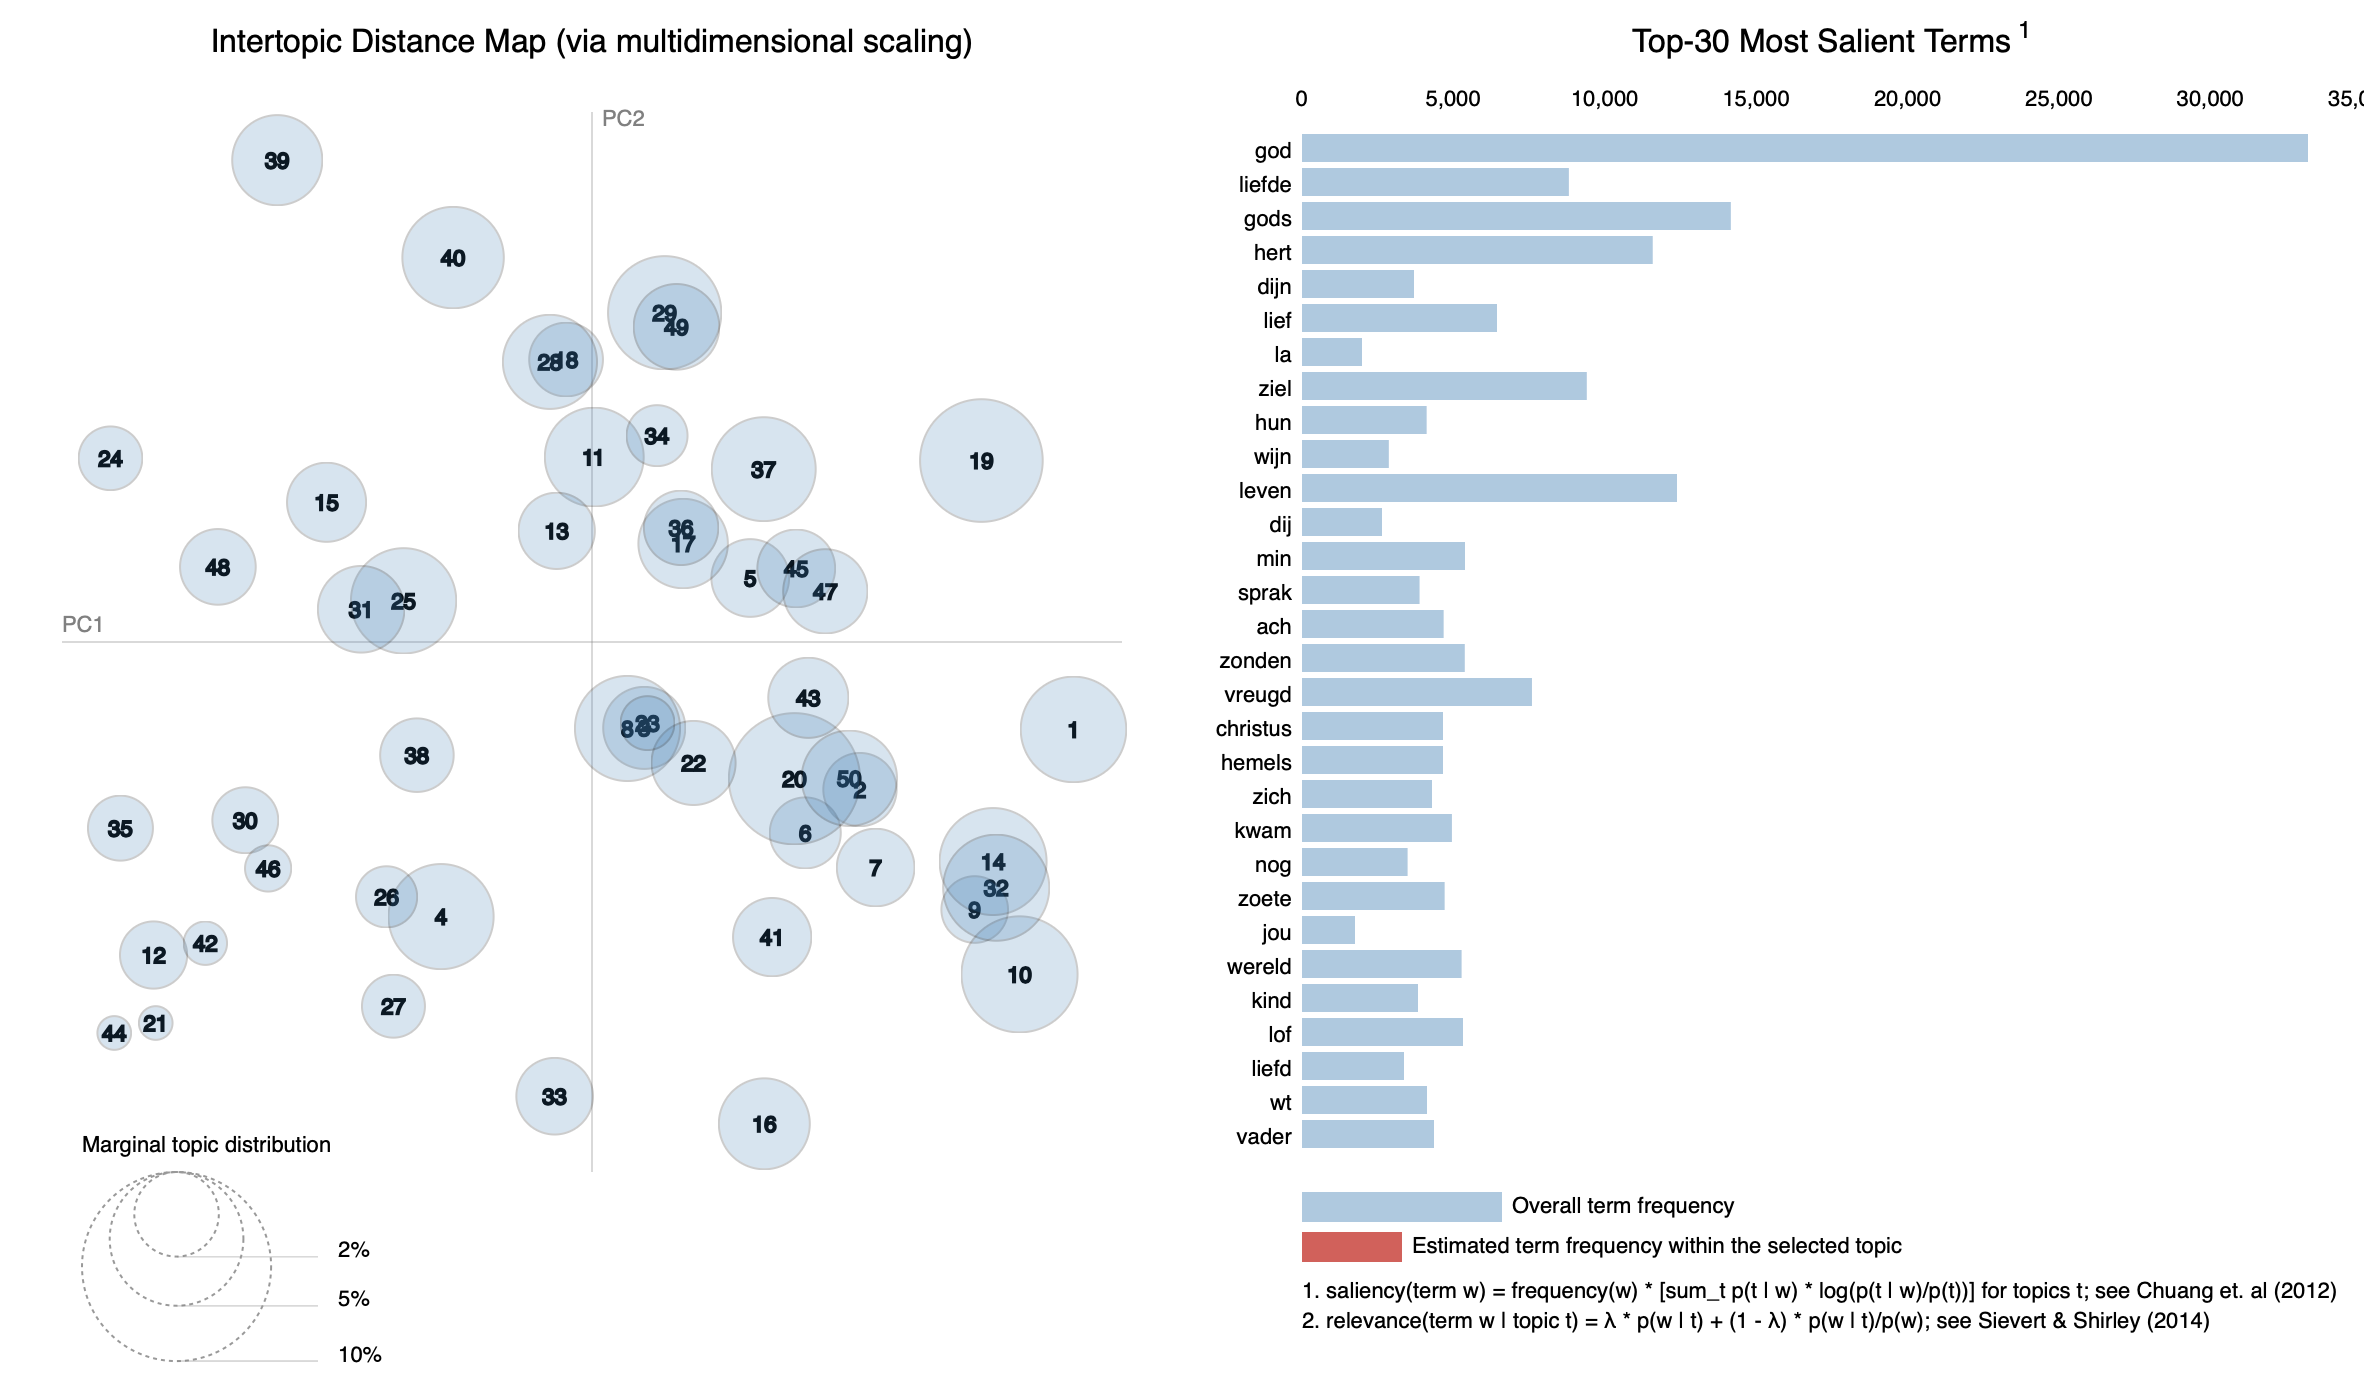
\includegraphics[scale=0.3]{VARD2_pyLDAvis}
	\caption{Visualization of topics in the VARD2-normalized corpus with \texttt{pyLDAvis}}
	\label{fig:pyLDAvisVARD2}
\end{figure}

\noindent Though the song contains various metaphorical phrases, such as \enquote{vrouw-voedster van de vuyle dartelheyt}, \enquote{oorsaeck van alle quadth}, \enquote{Wellust is een lastigh pack}, the song is still recognized as a song on wealth and soberness.

\begin{table}
	\begin{minipage}{0.5\textwidth}
		\begin{tabular}{ccl}
			\toprule
			Topic & Songs & Subject \\
			\midrule
			28             &  1151 & intangible religion \\
			39             &  1094 & love \& sadness \\
			38             &  1092 & love \& happiness \\
			18             &   878 & religion \\
			9              &   815 & religion \& old spelling \\
			0              &   756 & religion \& life \\
			24             &   618 & rejection \\
			2              &   591 & love \& tragedy \\
			13             &   591 & religion \\
			27             &   532 & world \& money \\
			6              &   521 & possessives \\
			31             &   518 & religion \\
			4              &   512 & religion \& happiness \\
			30             &   506 & love \\
			7              &   499 & God \& enemy \\
			14             &   498 & myth \& beauty \\
			21             &   477 & love \& happiness \\
			47             &   477 & bucolic songs \\
			44             &   465 & religion \& virtue \\
			40             &   464 & religion \& Jesus\\
			19             &   452 & verbs \\
			36             &   436 & religion \\
			49             &   432 & God \& country \\
			5              &   427 & Christmas \\
			12             &   422 & marriage \\
			\vdots & \vdots & \vdots \\
			\bottomrule
		\end{tabular}
	\end{minipage} \hfill
	\begin{minipage}{0.5\textwidth}
		\begin{tabular}{|ccl}
			\toprule
			Topic & Songs & Subject  \\
			\midrule
			\vdots & \vdots & \vdots \\						
			16             &   406 & good \& evil \\
			3              &   395 & verbs \\
			1              &   390 & religion \& Mary \\
			35             &   388 & religion \\
			46             &   386 & earthly life \\
			10             &   383 & suffer \& sadness \\
			29             &   378 & drinking \\
			48             &   377 & love \\
			23             &   355 & physical love \\
			34             &   351 & seducing \\
			32             &   340 & nation \& country \\
			42             &   339 & cross \& passion \\
			37             &   280 & nature \\
			8              &   268 & godly life \\
			11             &   253 & entertainment \\
			26             &   250 & money \& work \\
			15             &   248 & Old Testament \\
			17             &   244 & heaven \\
			22             &   227 & church \\
			25             &   201 & sea \\
			33             &   187 & ??? \\
			45             &   140 & trash \\
			41             &   124 & German \\
			43             &    97 & French \\
			20             &    66 & solfège \\
			\bottomrule
		\end{tabular}
	\end{minipage}
	\caption{Dominant topics in VARD2-normalized corpus (\textit{n} = 22,297)}
	\label{table:DomTopVARD2}
\end{table}

Topic 24 (Figure~\ref{fig:topic24VARD2}) is a remarkable one: I assigned the word \textit{rejection} to it. Several words, including the \enquote{weg}, \enquote{waarom} and especially the most prevalent \enquote{neen}, suggest that songs with this topic are about an unanswered love or the rejection of a lover. The song with this topic as its highest contribution shows this perfectly. Here I quote the first two stanzas (\texttt{id} = 10359):

\begin{quote}
	Ick ongheluckigh Vrijer,\\
	Hoe ben ick in de ly?\\
	Ick kan gheen Vrijster winnen,\\
	Hoe dapper dat ick vry,\\
	Sy achten 't maer voor grillen,\\
	't En klemt niet wat ick doe:\\
	Sal dit noch langher duuren,\\
	Ick wordt mijn leven moe.\\
	
	Ionghman waer toe dit klaghen,\\
	Ey! laet u grillen staen,\\
	'k En sagh van al mijn daghen\\
	Noyt sulcken vreemden Haen:\\
	Ghy reutelt en ghy rammelt,\\
	Als of ghy had' een gons,\\
	Ghy Bongioert selfs in jou Bocxsen,\\
	En leght die schult op ons.
\end{quote}

\noindent This song is a dialogue between Hylas and Phyllis. Hylas plays the role of an unlucky youngster who laments about his futile attempts in conquering a girl; Phyllis explains that girls do not like his rude approach. Another topic whose most representative song shows clearly the subjects of the songs belonging to this topic, is topic 32 on \textit{nation \& country} (Figure~\ref{fig:topic32VARD2}). The song with the highest contribution is a so called Geuzen song (\texttt{id} = 27769) from \textit{Een Nieu Geuse Lieden boecxken} (1578). Below the first three stanzas are quoted:

\begin{quote}
	Wel op, wel op Spangiaerden,\\
	Die nu in Brabant zijn,\\
	Hoe smaken u die ghebraden\\
	Daer toe den coelen wijn,\\
	Ghy moet naer Spangien met ghewelt,\\
	Sonder Paspoort, sonder gelt,\\
	Jochey, nu slaet dien Spangiaerts vry.\\
	
	In Brabant quamen sy dringhen\\
	Die Spaensche Jonckers wijs,\\
	Vlaendren wouden sy dwinghen,\\
	Die steden maecken prijs\\
	Of sy wolden hebben betaelt,\\
	Die leste penninck ongefaelt\\
	Jochey nu slaet de Spangiaerts vry.\\
	
	De Staten van den Lande,\\
	Die setten haer een dach,\\
	Wy sullen u wel betalen\\
	U Leeninghe corten af\\
	Soo moest ghy uyt den Lande gaen\\
	Die Spangiaerts riepen niet te verstaen\\
	Jochey, nu slaet de Spangiaerts vry.
\end{quote}

\begin{figure}
	\begin{minipage}[c]{0.48\linewidth}
		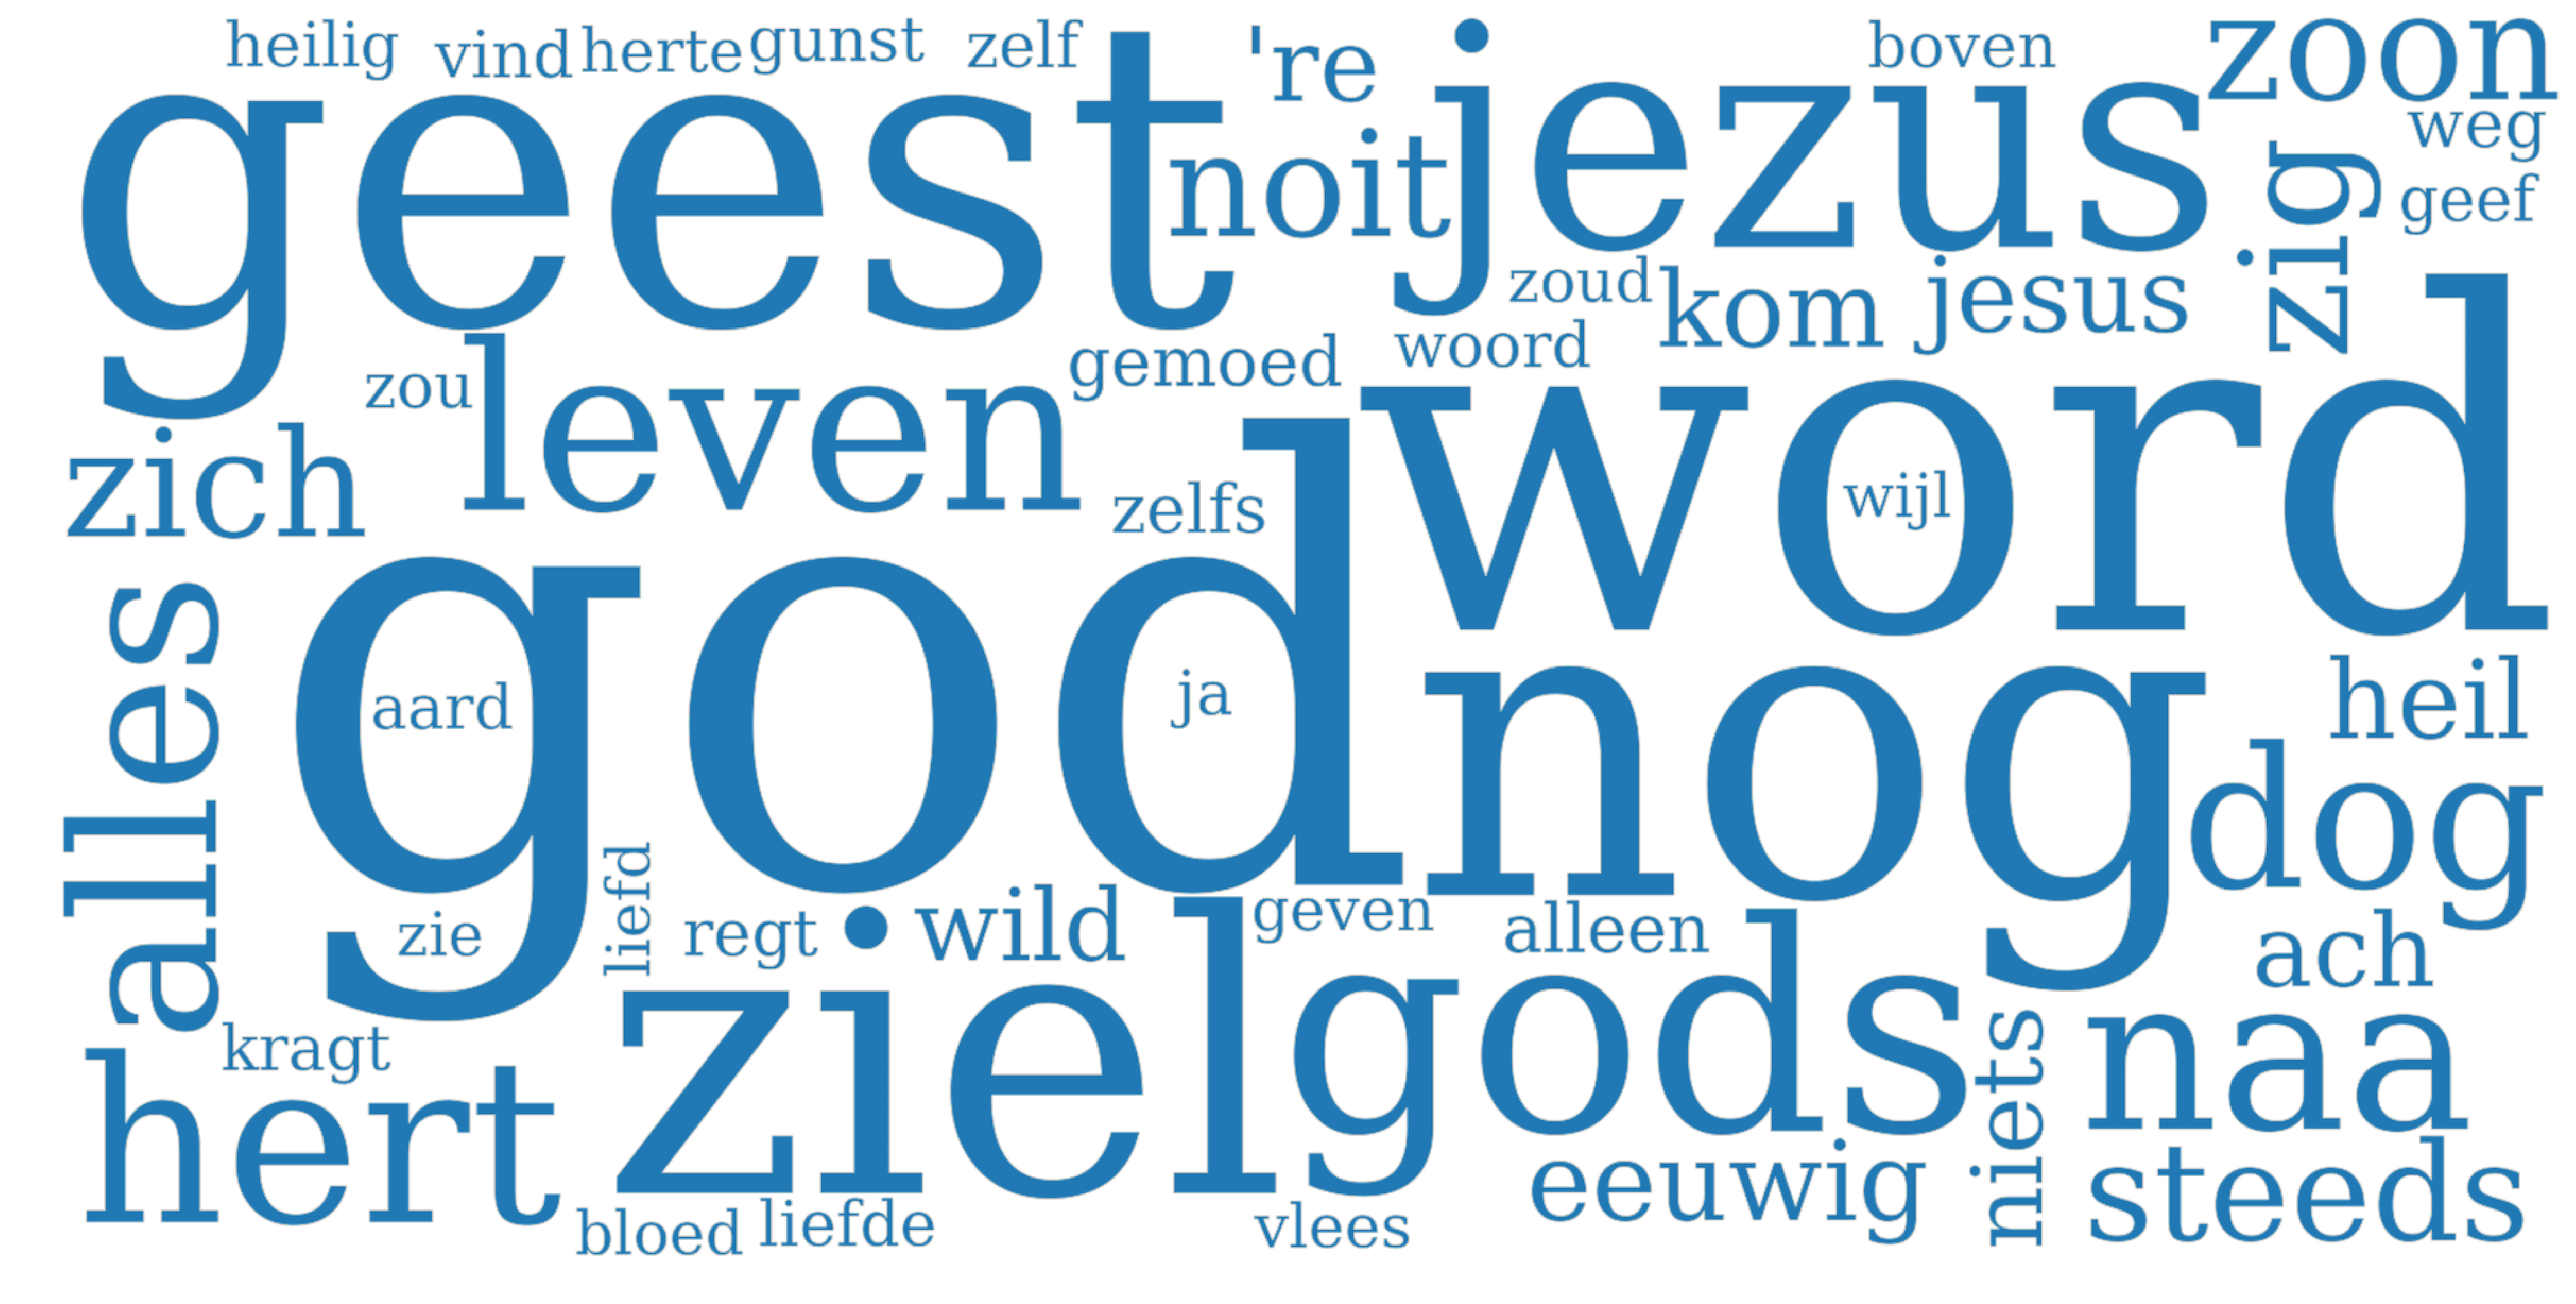
\includegraphics[width=\linewidth]{VARD2_topic28}
		\caption{\textit{religion \& intangibility} (28, VARD2)}
		\label{fig:topic28VARD2}
		\vspace{4ex}
	\end{minipage}%%
	\begin{minipage}[c]{0.48\linewidth}
		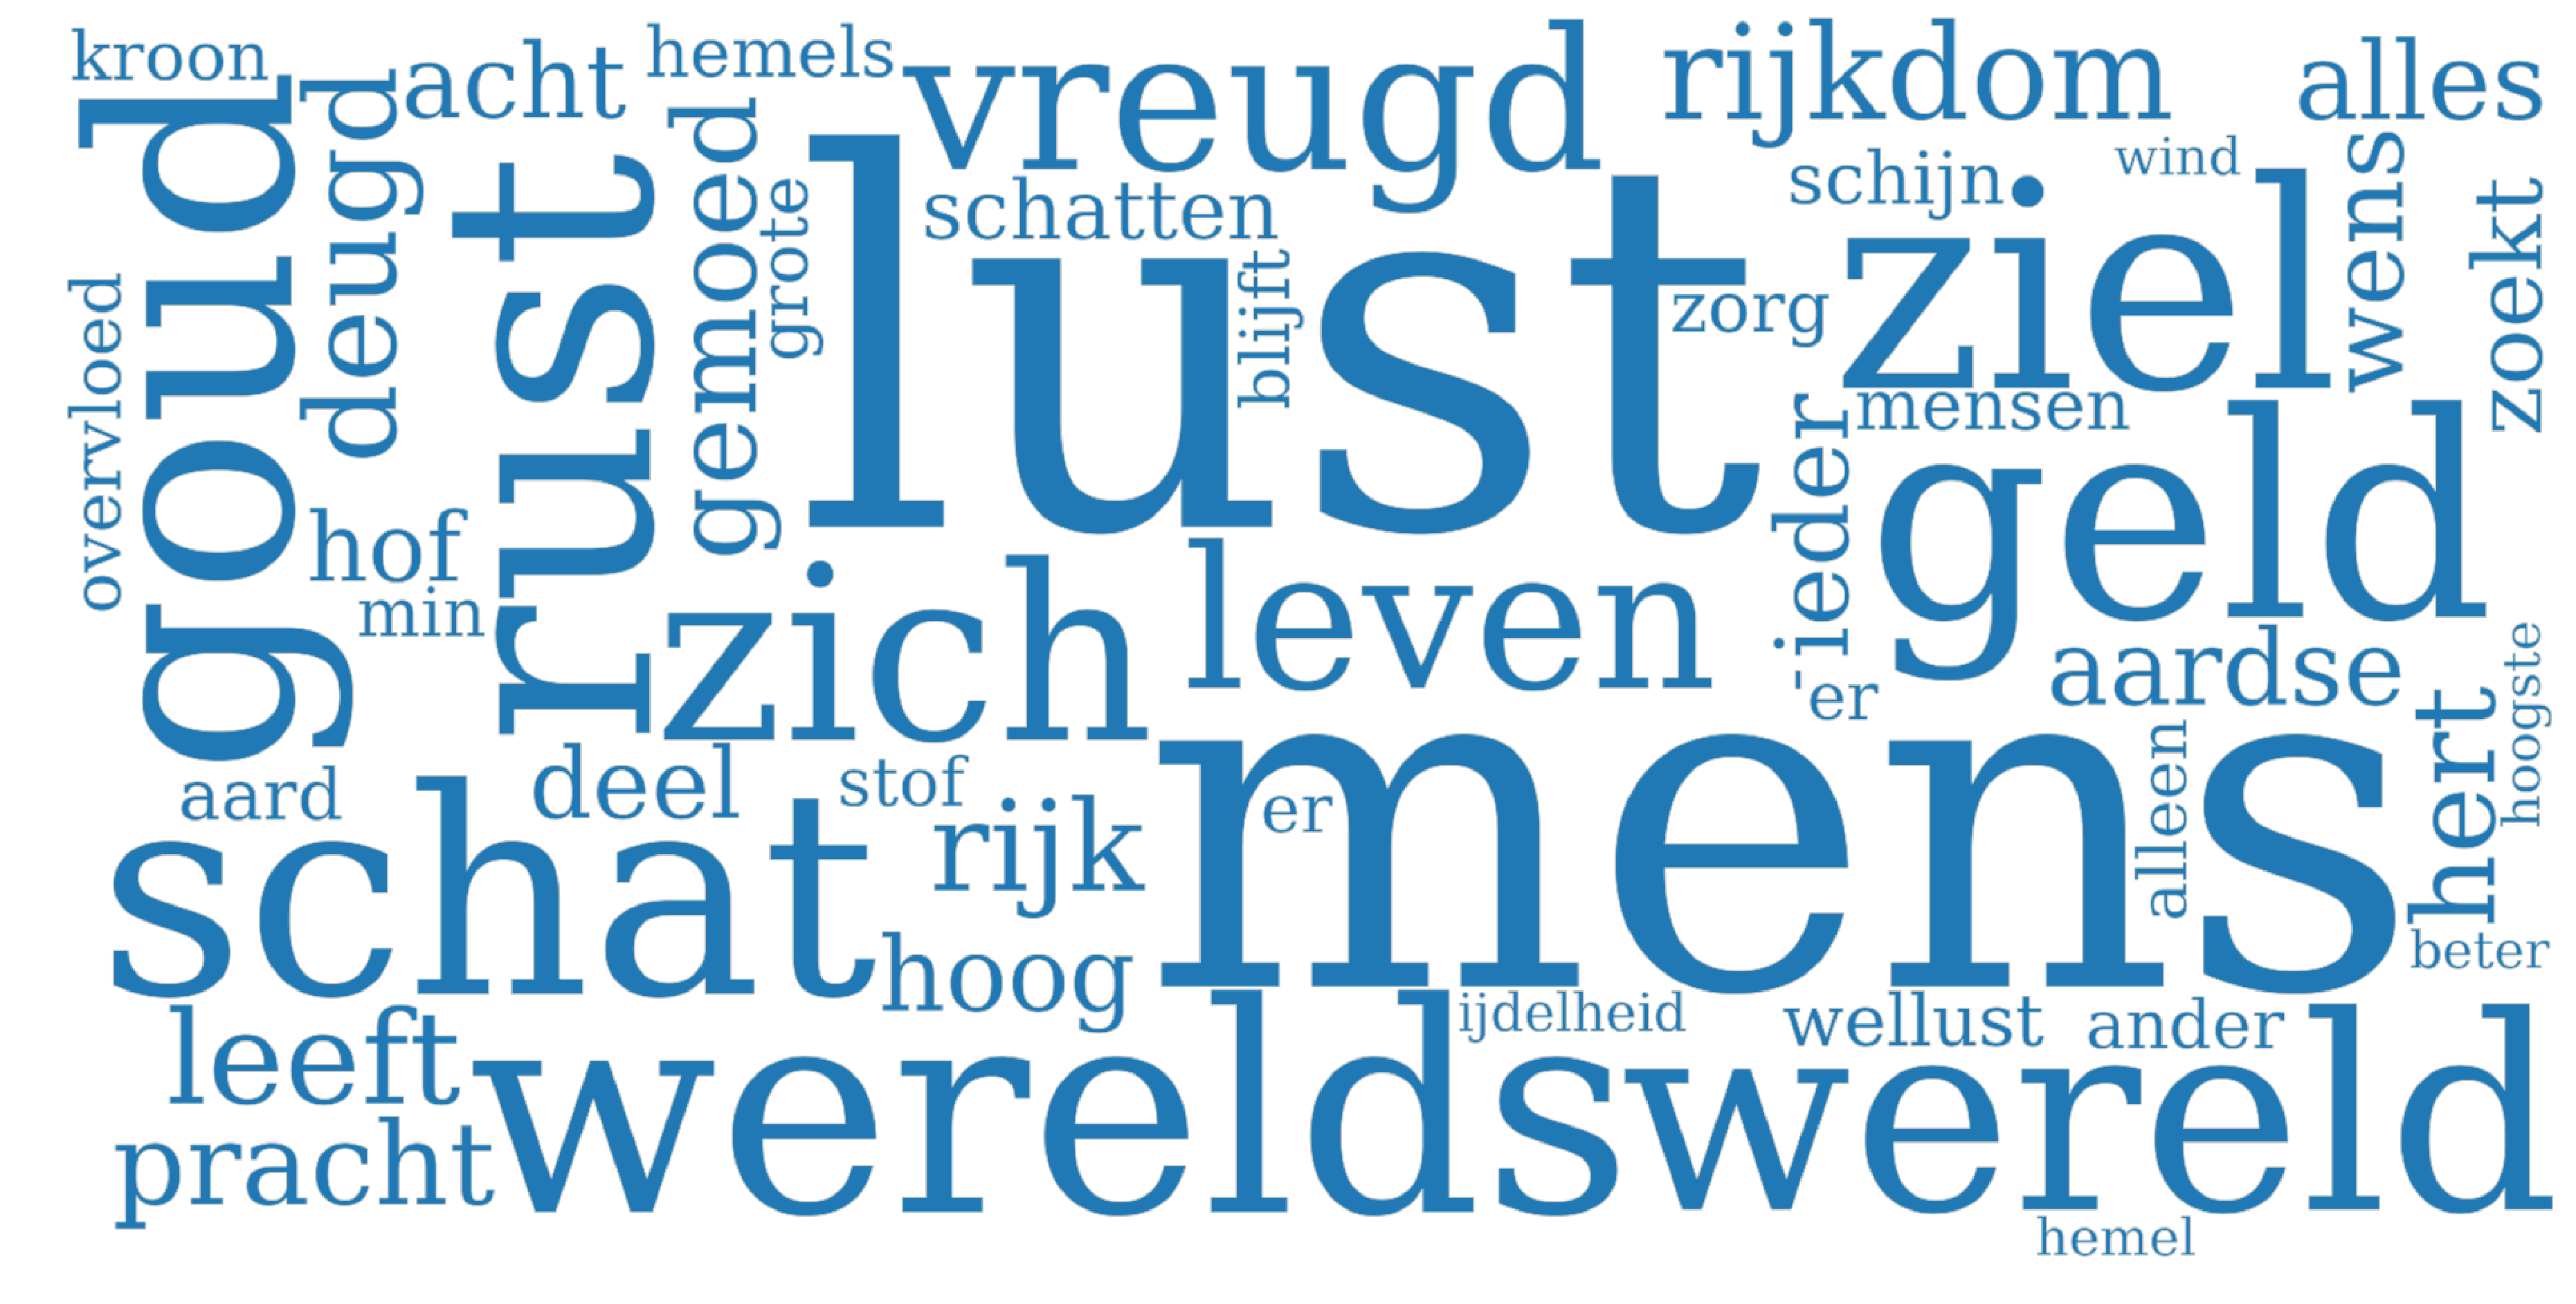
\includegraphics[width=\linewidth]{VARD2_topic27}
		\caption{\textit{world \& money} (27, VARD2)}
		\label{fig:topic27VARD2}
		\vspace{4ex}
	\end{minipage}%%
	\hfill
	\begin{minipage}[c]{0.48\linewidth}
		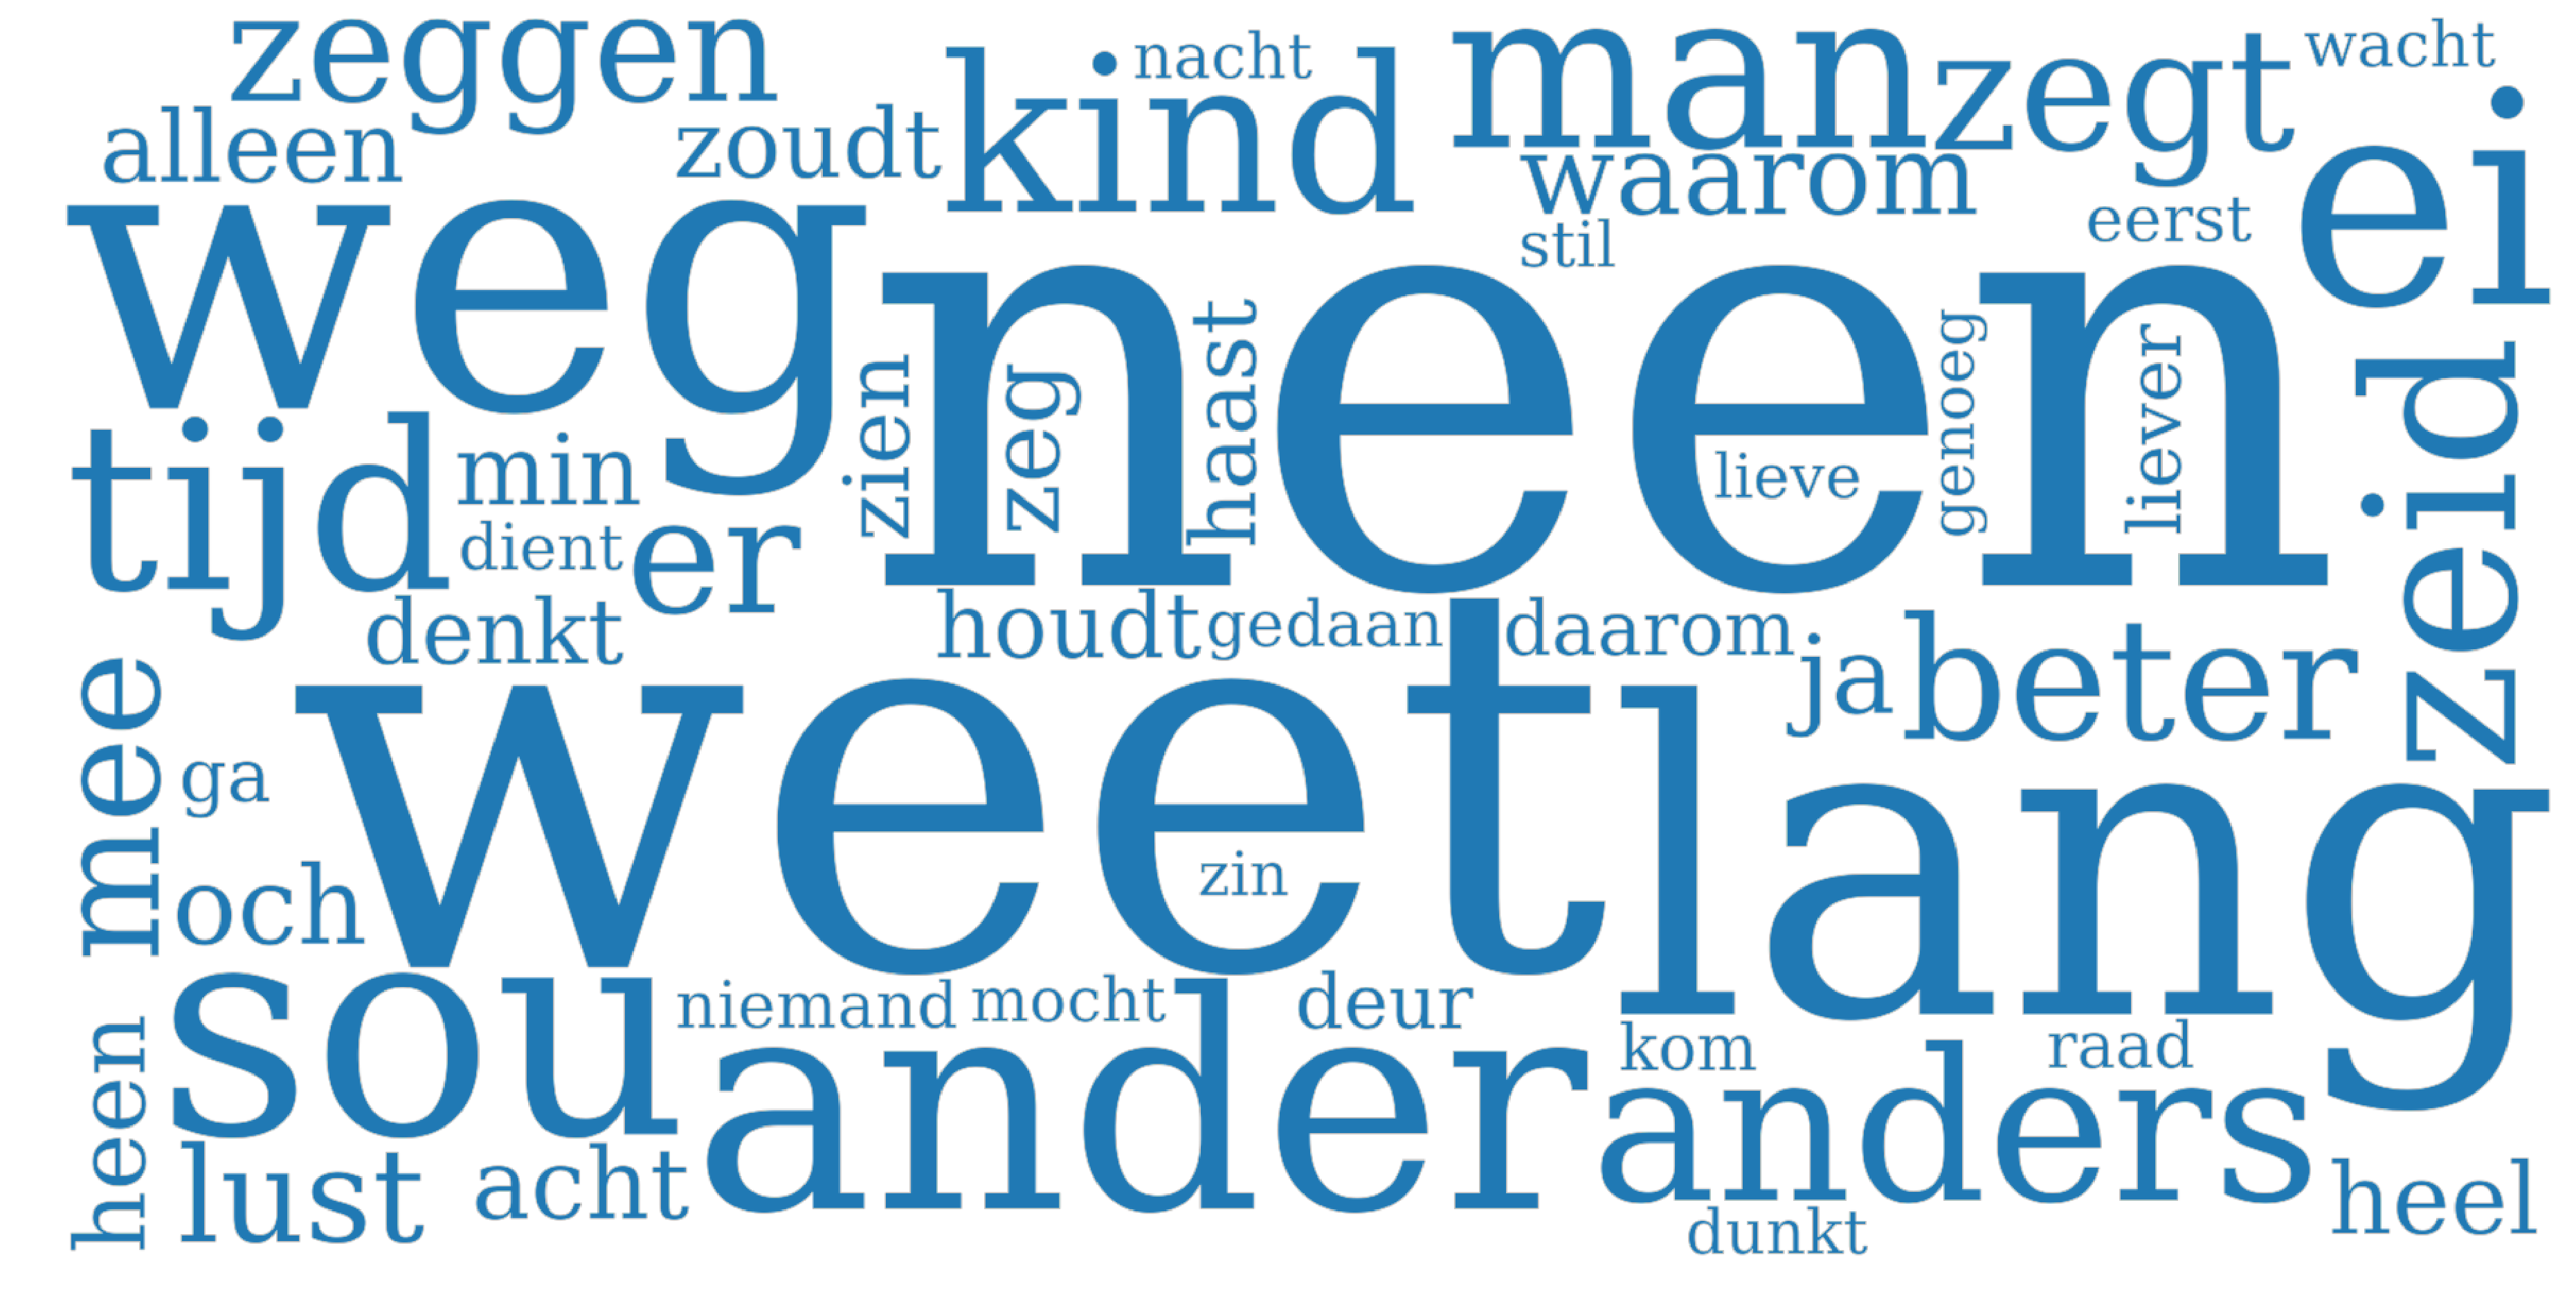
\includegraphics[width=\linewidth]{VARD2_topic24}
		\caption{\textit{rejection} (24, VARD2)}
		\label{fig:topic24VARD2}
		\vspace{4ex}
	\end{minipage}%%
	\begin{minipage}[c]{0.48\linewidth}
		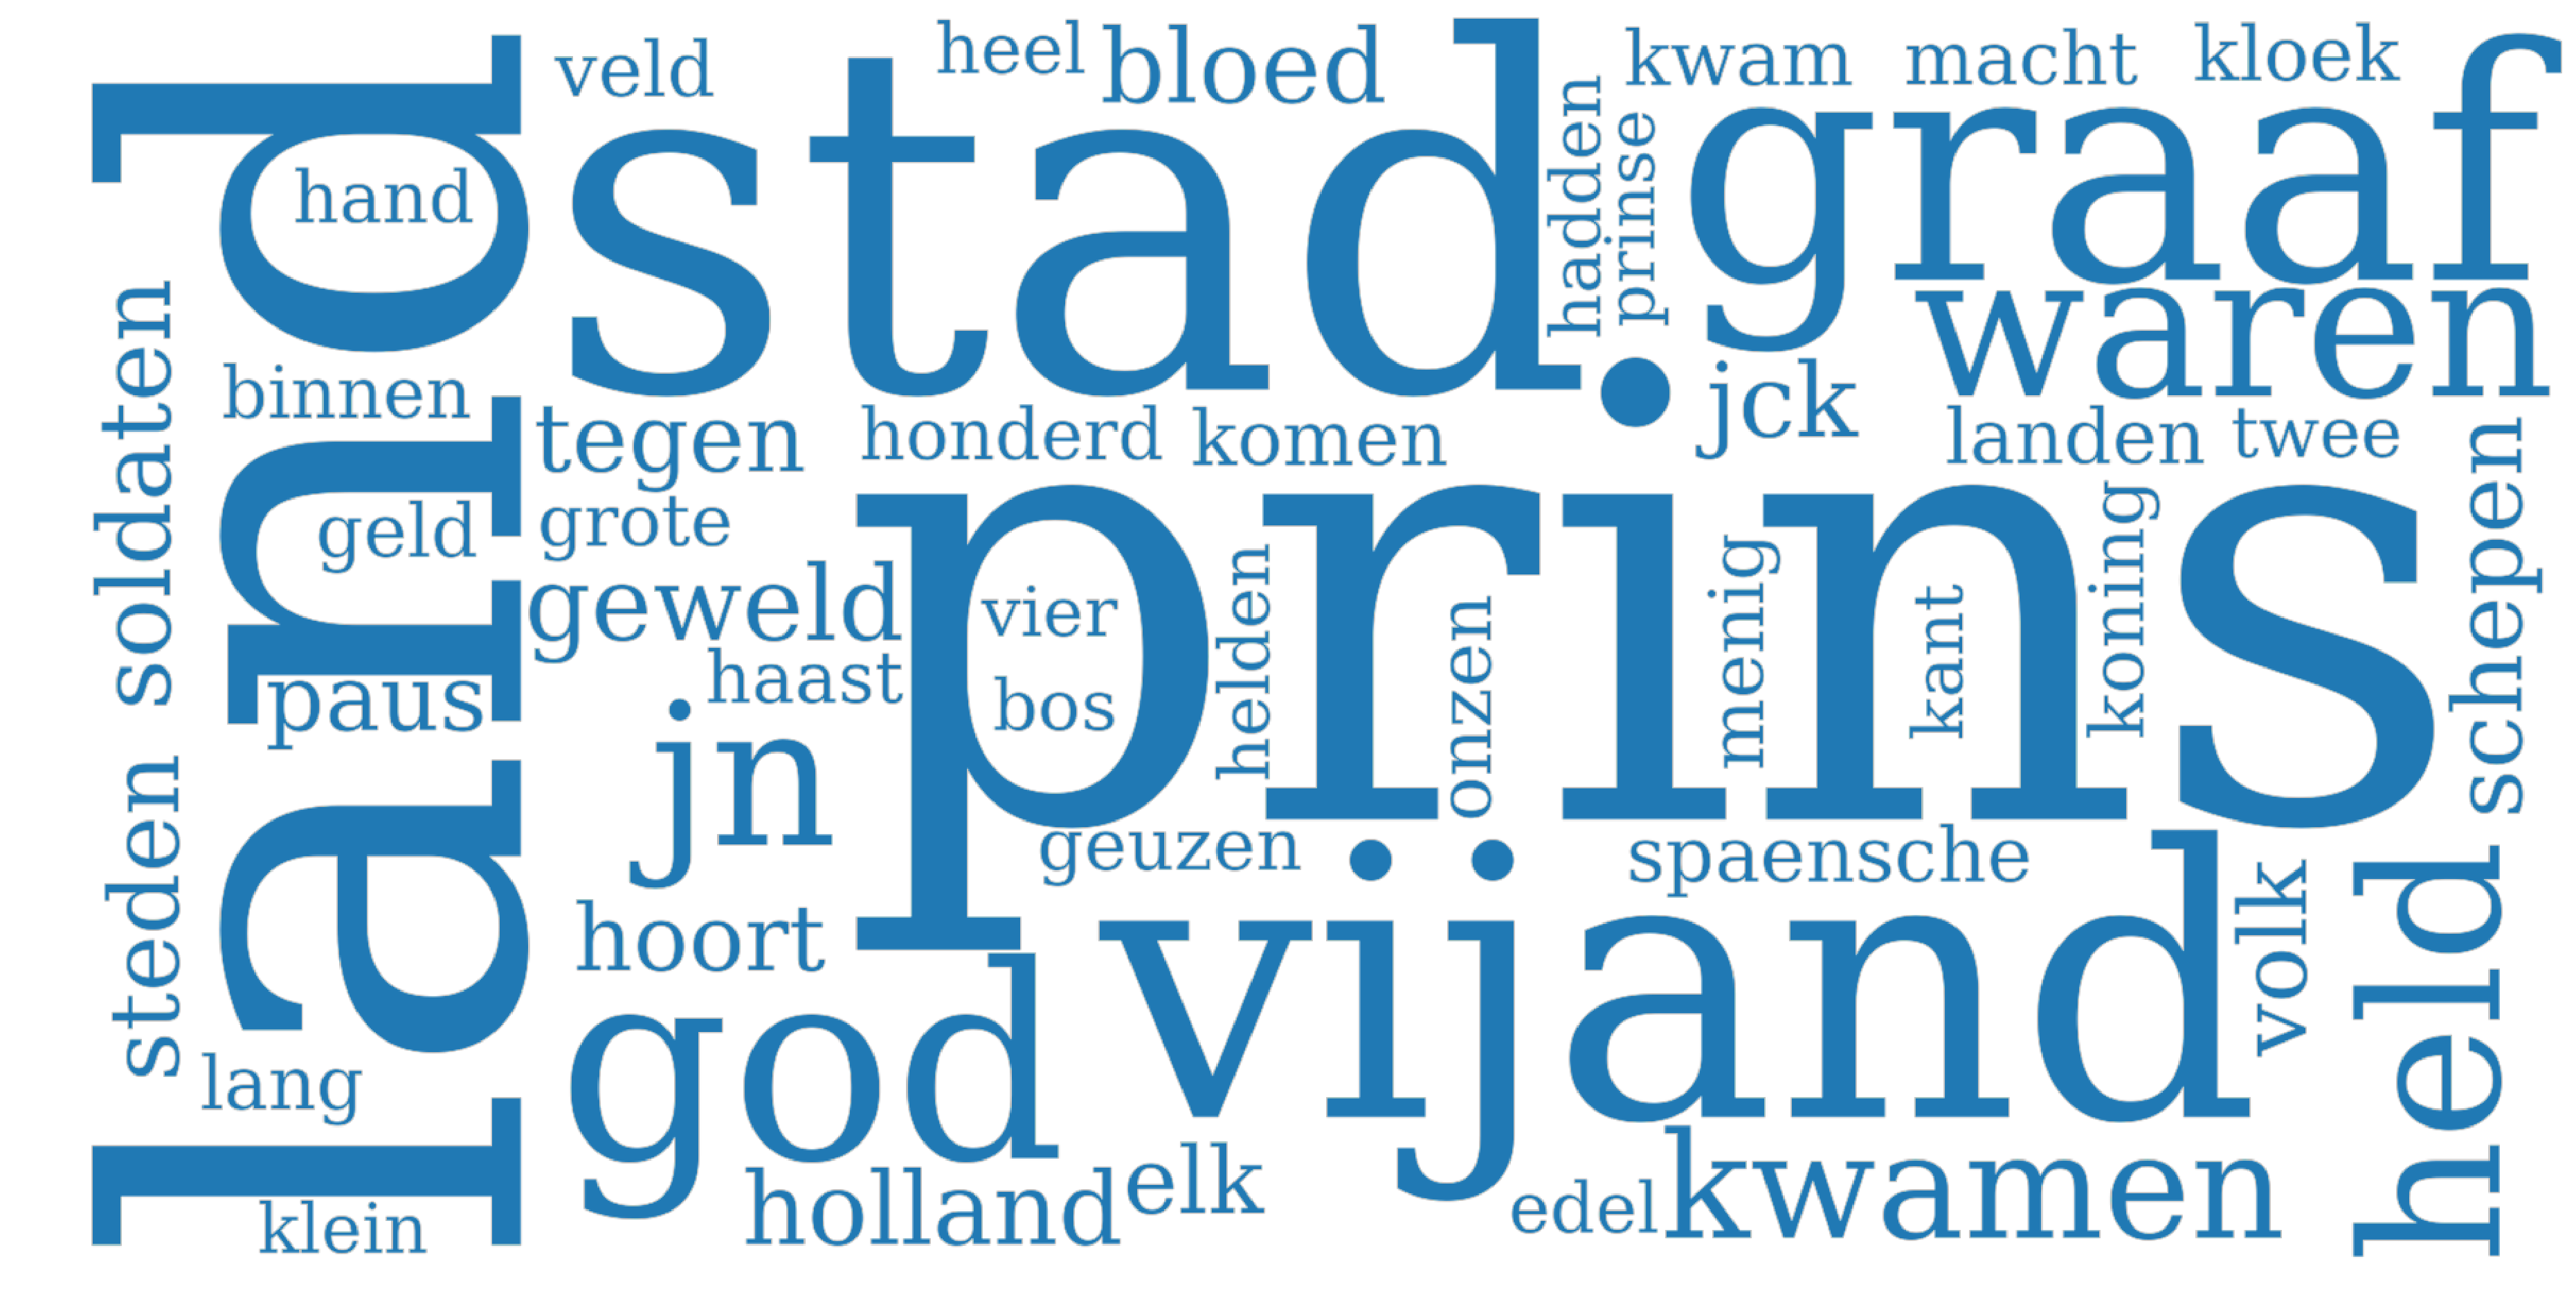
\includegraphics[width=\linewidth]{VARD2_topic32}
		\caption{\textit{nation \& country} (32, VARD2)}
		\label{fig:topic32VARD2}
		\vspace{4ex}
	\end{minipage}%%
\end{figure}

\noindent Geuzen songs were named after the Geuzen, the nickname for them who fought against the Spanish during the Dutch Revolt. In Geuzen songs, the motives for the battle against the Spanish were expressed, which is also the case in the song quoted above.

\section{Evaluating models}
Now that I have built three models from the three versions of my corpus, it is essential to evaluate the models and decide which one is the most worthwhile to continue my analysis with. It will come as no surprise anymore that the corpus normalized with the INL-tool is not worth the effort to investigate any further. Existing differences in words are smoothed out by wrong normalizations, resulting in inconclusive, resembling topics. The two remaining models are the one build from the original corpus, and the one build from the VARD2-normalized corpus. The biggest advantage of building topics from the original corpus, is that there is no risk in words losing their original meaning. However, this enormous word variation is at the same time a major disadvantage. The dictionary built from the original corpus is much larger than the dictionary from the VARD2-normalized corpus: 218,027 tokens versus 194,159 tokens. After discarding tokens that appear only one time, the difference is still considerable: 90,091 versus 77,114 tokens. This means that, when building topics from the original corpus, 12,977 words were considered as unique words, while, according to the VARD2-tool, these words were just variants of one of the other 77,114 words. From the  original corpus are therefore topics composed that are based on the time-specific spelling of the words. A negative consequence of this is that diachronic patterns in topical fluctuations are harder, or in fact impossible, to determine.

The VARD2-tool functions as a solution to that problem. The biggest advantage of this tool, compared to the INL-tool, is that I am able to verify which word was normalized to which word. VARD2 not only gives the normalized texts as .txt-output, but also every text as .xml-file, in which the performed normalizations are tagged. Moreover, a statistical file with data about how many words are normalized in each text, is created as well. Considering all this, I will continue my analysis with the version of the corpus that is normalized with the VARD2-tool. Although there are still a number of topics which can be considered as trash, the coherence of the words in these topics is the best I got.

It is now necessary to extend the corpus with the other songs containing the same \textit{incnormid}, resulting in a corpus of 43,772 songs, in which to every song the most dominant topic is assigned. I have used the following block of code for this:

\begin{lstlisting}
nlb = pd.read_csv("data/nlb.csv", sep=",")
nlb_timeset = nlb[(nlb["jaar_begin"] >= 1550) & (nlb["jaar_begin"] <= 1750)]
nlb_timeset = nlb_timeset[nlb_timeset["incnormid"] != 0] 

topics = pd.read_csv("VARD2_dominant_topic_per_song.csv", sep="\t", index_col=0)

msc = nlb_timeset.merge(topics, left_on="recordid", right_on="id")

nlb_timeset = nlb_timeset.loc[nlb_timeset["incnormid"].isin(msc["incnormid"])]

incs = msc.groupby("incnormid").first()[["dominant_topic", "perc_contribution"]]

topics = nlb_timeset.set_index("incnormid").join(incs).sort_values("incnormid")

topics = topics.reset_index()
\end{lstlisting}

\noindent The question is how the distribution of topics changes, now the size of the corpus almost has doubled. In Table~\ref{table:DomTopVARD2extended}, the new numbers of songs are presented. There are some changes in the ranking, but mostly because of religious topics that have taken over the Top10. A topic with a remarkable rise, is topic 32, on \textit{nation \& country}. Originally, there were 340 songs with this topic as the most prevalent one, but that number has increased to 1221. Earlier I showed that the song that represented this topic at best, was a Geuzen song. The expansion of this topic can be explained by the fact that song books with the so called Geuzen songs were reprinted a lot during the Dutch Revolt.

\begin{table}
	\begin{minipage}{0.5\textwidth}
		\begin{tabular}{ccl}
			\toprule
			Topic & Songs & Subject \\
			\midrule
			9              &            3936 & religion \& old spelling \\
			31             &            1966 & religion \\
			0              &            1848 & religion \& life \\
			28             &            1700 & intangible religion \\
			39             &            1671 & love \& sadness \\
			18             &            1631 & religion \\
			38             &            1607 & love \& happiness \\
			13             &            1403 & religion \\
			6              &            1277 & possessives \\
			32             &            1221 & nation \& country \\
			2              &            1073 & love \& tragedy \\
			24             &            1062 & rejection \\
			30             &            1038 & love \\
			1              &            1029 & religion \& Mary \\
			5              &            1021 & Christmas \\
			44             &             944 & religion \& virtue \\
			27             &             869 & world \& money \\
			12             &             841 & marriage \\
			47             &             787 & bucolic songs \\
			40             &             771 & religion \& Jesus \\
			48             &             767 & love \\
			8              &             755 & godly life \\
			46             &             752 & earthly life \\
			19             &             744 & verbs \\
			4              &             693 & religion \& happiness \\
			\vdots & \vdots & \vdots \\
			\bottomrule
		\end{tabular}
	\end{minipage}
	\begin{minipage}{0.5\textwidth}
		\begin{tabular}{|ccl}
			\toprule
			Topic & Songs & Subject \\
			\midrule
			\vdots & \vdots & \vdots \\
			36             &             686 & religion \\
			17             &             683 & heaven \\
			7              &             675 & God \& enemy \\
			14             &             655 & myth \& beauty \\
			49             &             646 & God \& country \\
			10             &             642 & suffer \& sadness \\
			34             &             628 & seducing \\
			21             &             625 & love \& happiness \\
			3              &             618 & verbs \\
			42             &             616 & cross \& passion \\
			23             &             602 & physical love \\
			29             &             590 & drinking \\
			16             &             572 & good \& evil \\
			15             &             546 & Old Testament \\
			37             &             501 & nature \\
			33             &             492 & ??? \\
			26             &             418 & money \& work \\
			35             &             410 & religion \\
			11             &             392 & entertainment \\
			22             &             329 & church \\
			25             &             312 & sea \\
			45             &             302 & trash \\
			41             &             170 & German \\
			43             &             148 & French\\
			20             &             108 & solfège\\
			\bottomrule
		\end{tabular}
	\end{minipage}
	\caption{Dominant topics in VARD2-normalized corpus (\textit{n} = 43,772)}
	\label{table:DomTopVARD2extended}
\end{table}

A methodical choice that needs some critical evaluation, is the fact that I picked the most dominant topic for each song and discarded the rest. It is possible, though, that a certain topic is very often the second-popular topic of a song. If that topic is rarely the most popular topic, it will end at the bottom of the ranking as stored in Tables~\ref{table:DomTopVARD2} and~\ref{table:DomTopVARD2extended}, although it can be a rather prevalent topic within the corpus. Another hypothesis, which can not be tested with the current method and the results arising therefrom, is that certain topics often occur together in a Top3 of topic contributions of a song. To get more insight in these trends, I extracted the Top3 topics of each song with the following code:

\begin{lstlisting}
transformed_docs = lda.load_document_topics()
docs = [[texts[indx]] + [p[1] for p in doc] for indx, doc in enumerate(transformed_docs)]
composition = pd.DataFrame(docs, columns=["document_id"] + ["topic {}".format(x) for x in range(0, N_TOPICS)])

arr = np.argsort(-composition.values, axis=1)
df1 = pd.DataFrame(composition.columns[arr], index=composition.index)

top3topics = df1[[0, 1, 2]].copy()
top3topics.columns = ["top1", "top2", "top3"]

songstop = nlb_timeset.merge(top3topics, left_on="recordid", right_on="id")
nlb_timeset = nlb_timeset.loc[nlb_timeset["incnormid"].isin
(songstop["incnormid"])]
incstop = songstop.groupby("incnormid").first()[["top1", "top2", "top3"]]

top3topicsong = nlb_timeset.set_index("incnormid").join(incstop).
sort_values("incnormid")
top3topicsong = top3topicsong.reset_index()
\end{lstlisting}

\noindent The result is a dataframe with 43,772 rows, where for each song (i.e. each row) the Top3 dominant topics are stored in columns. I grouped the topics that were in the second position of the Top3, and stored the most frequent ten of them in Table~\ref{table:SecondandThirdPopularTopics}. It turns out that from the Top10 second-popular topics, five topics were in the Top15 popular topics as well. They are all on religion.\footnote{Topics 31 (\textit{religion}), 9 (\textit{religion \& old spelling}), 18 (\textit{religion}), 0 (\textit{religion \& life}) and 24 (\textit{rejection}).} From the other five topic from the Top10 second-popular topics, two topics were composed of \textit{verbs}.\footnote{Topics 19 and 3.} The three other topics in the Top10 second-popular topics were on \textit{suffer \& sadness}, \textit{religion} and \textit{God \& enemy}. From the Top10 third-popular topics, eight topics were in the Top10 second-popular topics as well. The two \enquote{new} topics are topic 15 on the \textit{Old Testament} and topic 21 on \textit{love \& happiness}. I conclude therefore that, except the topics on \textit{God \& enemy} and the \textit{Old Testament}, the Top3 does not bring new topics to attention.

\begin{table}[]
	\centering
	\begin{tabular}{lll|lll}
		\toprule
		Topic 2 & Songs & Subject & Topic 3 & Songs & Subject  \\
		\midrule
		19 & 3456 & verbs 	&	19 &   4513 & verbs \\
		31 & 2295 & religion & 18  &  2244 & religion  \\
		9 & 2166 & religion \& old spelling & 10   & 1988 & suffer \& sadness\\
		18 & 2109 & religion & 0 & 1928 & religion \& life \\
		0 & 1724 & religion \& life & 3 & 1820 & verbs \\
		10 & 1693 & suffer \& sadness & 24 & 1790 & rejection \\
		24 & 1659 & rejection & 7 & 1659 & God \& enemy \\
		3 & 1658 & verbs & 36 & 1433 & religion \\
		36 & 1564 & religion & 15 & 1254 & Old Testament \\
		7 & 1342 & God \& enemy & 21 & 1235 & love \& happiness \\
		\bottomrule      
	\end{tabular}
	\caption{Top10 with second- and third-popular topics}
	\label{table:SecondandThirdPopularTopics}
\end{table}

The answer to my question what the most dominant topics in my corpus are, is \enquote{religion and something}, for sure. That result is not surprising at all: I already knew from the distribution of categories (Table~\ref{table:SongsCat}) that I could expect lots of topics concerning \enquote{religion}. However, since this category assigning has been in some cases quite general and arbitrary, the topic modeling method could give more insight in topical subdivisions within a genre. For some reason, LDA was able to distinguish songs that were merely on religion and happiness from songs that were merely on religion and virtue. The same applies to songs from the category \enquote{love and sex}. In the Dutch Song Database, thousands of songs are placed in this category, leaving no room for difference between songs on love and happiness, songs on love and sadness, or songs on rejection. Building a topic model has resulted in uncovering differences within the wide-ranging genres of songs. The next step I want to take in this thesis is how these topics in song lyrics fluctuate over time. Are songs on love and happiness and songs on love and sadness rising at the same time, or is the one a reaction to the other? When are songs on God and country becoming prevalent? Are there certain religious topics that disappear over time, being replaced by others? Can I indicate certain historical or cultural events that drive these trends? And how do my observations relate to prevailing theses in current research on the role of literature in the early modern centuries? Can I confirm that literature functions as a constructor of identity? Is the relation between politics and literature indeed reflected in my results? Does a certain ideology emerge from topics, and if so, which one? Are song topics becoming more and more variate over time, as well as the audience of songs? In the next chapter I will try to find an answer to these questions.





	\chapter{Roles of literature}

In this chapter I examine how the composed topics and their dynamics over time relate to prevailing theses drawn from contemporary qualitative research on the role of early modern literature, which I already discussed in Chapter 1, \textit{Introduction}. I discuss each claim in more detail, after which I explore whether the claim can be validated with the obtained results.

\section{Literature and ideology}
In the Introduction, I already discussed how literature is seen as a propagator of an ideology and how this is the case for the literature of the pietistic tradition. I also made clear in the previous chapter, that religion is by far the most dominant topic in my corpus. From the fifty topics that were built, eighteen have, more or less, something to do with religion. Regarding the Top10 most dominant topics, six of them are on religion. In Figure~\ref{fig:religion}, I plotted the evolution of these six topics over time. The y-axis shows the number of songs with a certain topic as their most dominant topic; the x-axis shows the development of a topic's popularity through time. Table~\ref{table:DomTopVARD2extended} already showed that topic 9 was by far the most dominant topic in my corpus. Figure~\ref{fig:religion} makes clear that this topic was mainly popular in the sixteenth century: it even almost disappears after 1650. There is a clear explanation for that, to which I already referred in assigning the subject \textit{religion and old spelling} to this topic. It contains words in a typical fifteenth and sixteenth-century spelling, ages in which no clear difference between the printed letters \enquote{v}, \enquote{w} and \enquote{u} existed, resulting in words such as \enquote{wt}, \enquote{bouen}, \enquote{uan}, \enquote{verheuen}, and \enquote{blijuen}. These words were not normalized by the VARD2-tool. An explanation for this is that the tool was trained on more recent texts (dating from 1637 and 1657), in which words were spelled according to more modern spelling conventions. Variants that were common in earlier centuries, were therefore probably not included in the variant-list. Another reason might be that these interchangeable letters, such as \enquote{v}, \enquote{u}, and \enquote{w}, are mainly a result of poorly transcribed prints. It can be said anyway that this topic 9 is not actually a topic, but merely a cluster of old-fashioned words that were still used between 1550 and 1625, and that these words disappear from the vocabulary of song lyrics when the seventeenth century endures.

\begin{figure}[hbt!]
	\centering
	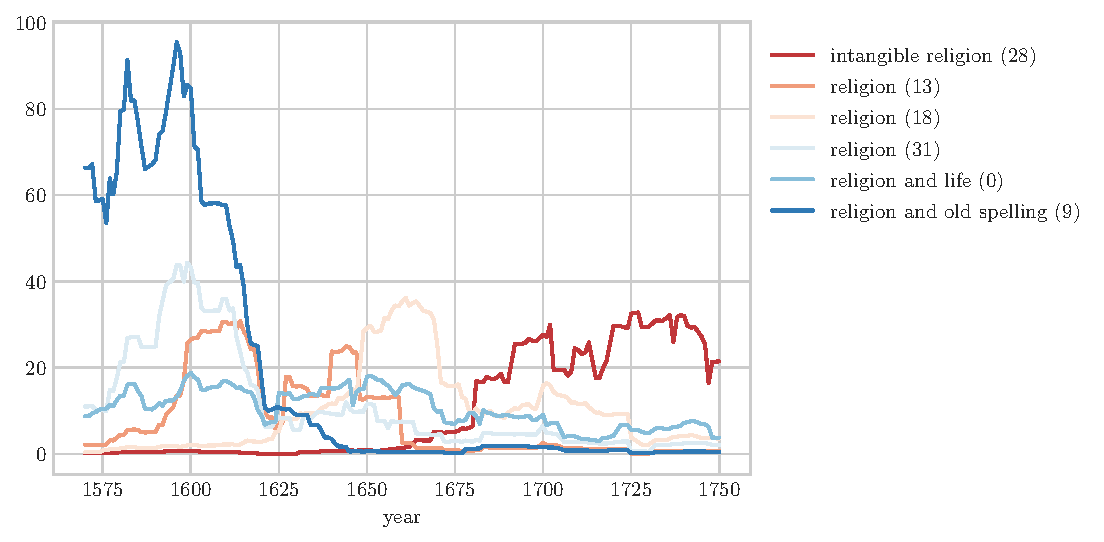
\includegraphics[scale=0.8]{religion}
	\caption{Topics on religion from the Top10}
	\label{fig:religion}
\end{figure}

Dynamics within the other five topics can be easier observed in a graph without topic 9. This plot (see Figure~\ref{fig:religion_min_9}) shows that the topics 13, 18 and 31, to which I was not able to assign a more detailed subscription than \textit{religion}, follow each other roughly. It starts with topic 31, peaking just before 1600, succeeded by topic 13 which culminates in the first half of the seventeenth century. Topic 18 closes the row, peaking in the second half of the seventeenth century. Looking in more detail to the words from which the topics were composed, does not give that much insight, but in the Intertopic Distance Map, made with \texttt{pyLDAvis} (Figure~\ref{fig:pyLDAvisVARD2}), topics 13 and 31 overlap very much in the bottom right quadrant. This overlap can also be observed when looking at their graph lines: both topics peak almost at the same time. Topic 18 is positioned in the upper right quadrant in Figure~\ref{fig:pyLDAvisVARD2}, the same quadrant where topic 28 is located: the topic on \textit{intangible religion} that succeeds topic 18, according to the plot in Figure~\ref{fig:religion_min_9}. There is a clear trend in the graph line of topic 28: until 1650 this topic hardly exists, but afterwards the line shows a quickly increasing slope. Until 1750, where my corpus ends, this topic on \textit{intangible religion} dominates. I already explained in the previous chapter that, in this topic, words prevail that are related to the intangible aspects of the Christian faith.

\begin{figure}[hbt!]
	\centering
	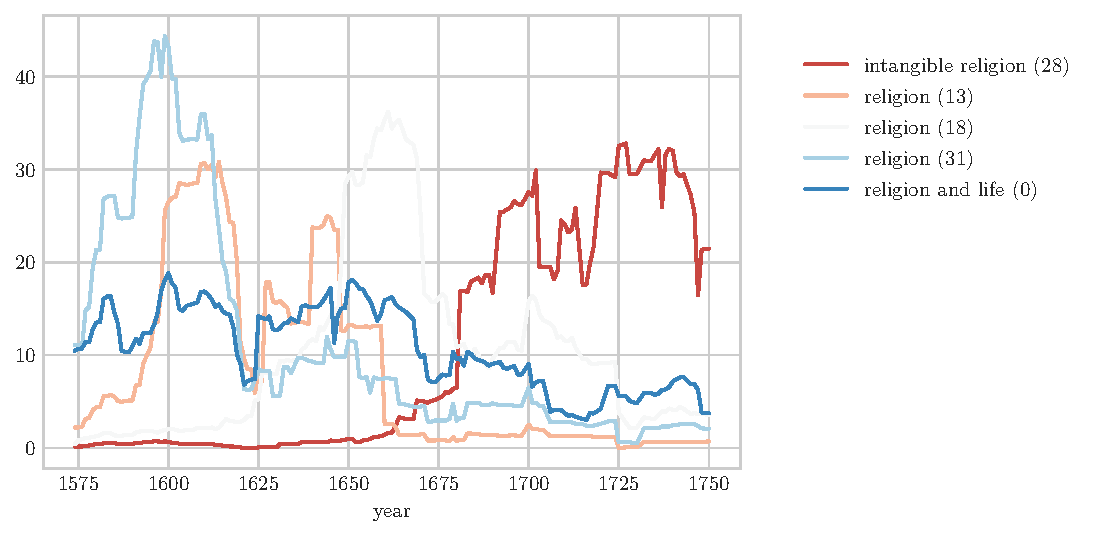
\includegraphics[scale=0.8]{religion_min_9}
	\caption{Topics on religion from the Top10 (except topic 9)}
	\label{fig:religion_min_9}
\end{figure}

\begin{figure}[hbt!]
	\centering
	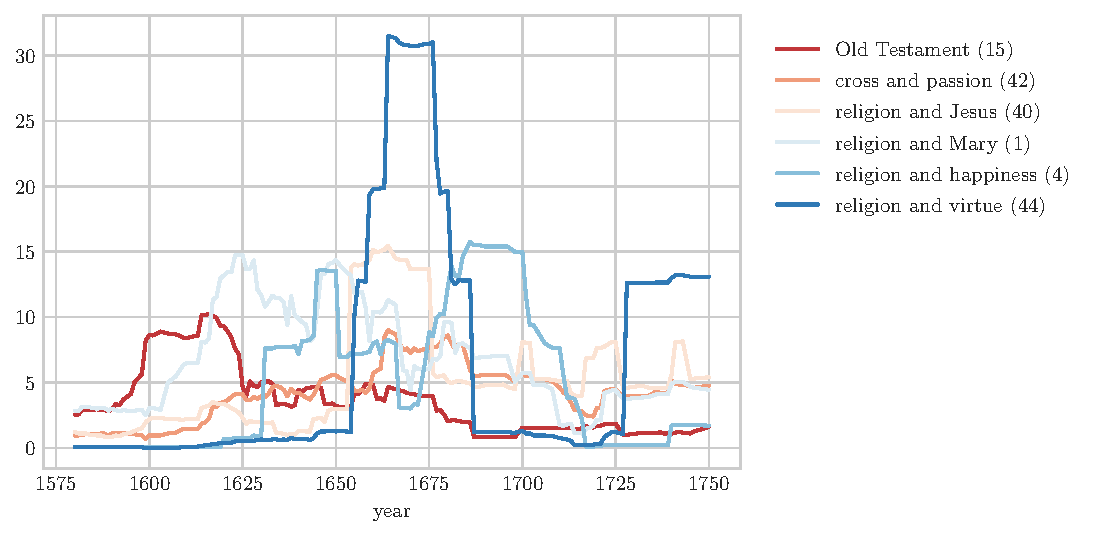
\includegraphics[scale=0.8]{religion2}
	\caption{Topics on religion from the lower parts of the chart}
	\label{fig:religion2}
\end{figure}

Since the sudden increase of this topic coincides with the rise of the pietistic tradition in the Low Countries called the Further Reformation, topic 28 clearly represents one of the two trends Porteman and Smits-Veldt determined in literary texts from this movement. On the one hand, literary texts with a focus on a sanctification on society and all aspects of life, prevailed. On the other hand, texts appeared in which the personal lived experience with God was described and expressed. These latter are brought together in topic 28. Figure~\ref{fig:religion2} shows that the other religious topics, which were located lower in the chart, do not demonstrate a striking curve, except the \enquote{Domtower-ish} shape of topic 44, belonging to \textit{religion and virtue}. Since the sudden rise of this topic is located in the second half of the seventeenth century as well, this seems to fit with the first trend of the literary texts from the Further Reformation that Porteman and Smits-Veldt determined. \autocite[658]{porteman_een_2009} Dominant words in this topic that confirm these thoughts, are \enquote{deughden}, \enquote{bidt}, \enquote{leven}, and \enquote{vroom}. The twofold ideology the advocates of the Further Reformation wanted to propagate according to contemporary research, is cleary represented in the obtained quantitative results.

\section{Literature and poetics}
I expect the relationship between literature and poetics to be most apparent in love topics that can be related to Petrarchism. Francesco Petrarca (1304 - 1374), godfather of this movement, was an Italian poet from the fourteenth century, who became famous all over Europe during the early modern centuries. One of the reasons for this was because he started to write poetry in the Italian vernacular, and based on the classics. This was a great inspiration for Dutch poets in the sixteenth and seventeenth century, who were searching for their own identity, during a war for political and religious independence.\autocite[17]{porteman_een_2009} The other reason for Petrarca's fame in the Netherlands was the popularity of his poetry on love. Distinctive of Petrarca's love sonnets, was the worship of a charming but unreachable woman. As a result of that, love always causes both happiness and pain in his poems. The physical beauty of the beloved is often described, using natural metaphors and mythological references. The lover owns a split personality, and often struggles with suicidal tendencies.\autocite{bork_algemeen_2012} 

Regarding the results obtained in the previous chapter, the second-largest overarching category of topics is love. The two most dominant topics in this category, are two contradictory ones: topic 39 is on \textit{love and sadness}, topic 38 is on \textit{love and happiness}. In Figure~\ref{fig:love} I plotted the two topics through time, which shows an interesting pattern. What immediately stands out, is that the topics only start to occur around 1630. From that point in time, \textit{love and sadness} is the most dominant topic, culminating around 1660, but decreasing quickly afterwards. Around 1710, the line of topic 38 on \textit{love and happiness} suddenly rises, and rapidly becomes the dominant one of the two love topics. This plot suggests that song with negative emotions are replaced by songs with a more light-footed view on love. The question is if that trend is confirmed by other topics on love. Therefore I included more love-topics to the plot, resulting in the graph of Figure~\ref{fig:love_extended}. Prior to topic 39, topic 2 starts the list of topics on love. This topic, on \textit{love and tragedy}, dominates between 1575 and 1630. What follows, is a couple of overlapping peaks, all culminating around 1660, with the topic on \textit{love and sadness} as most dominant one. The smaller peaks belong to \textit{rejection}, \textit{seducing} and \textit{physical love}.

\begin{figure}[hbt!]
	\centering
	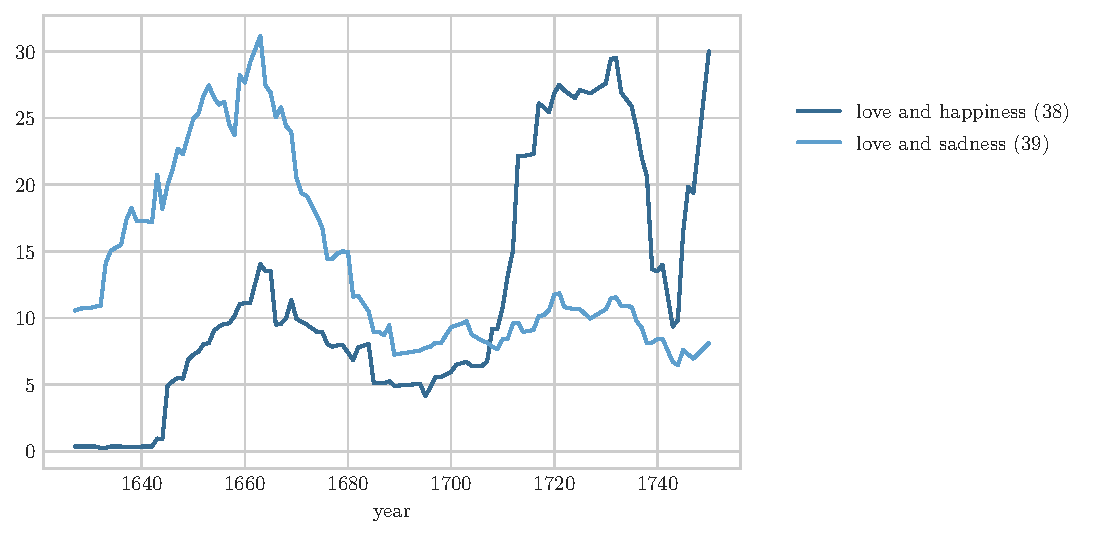
\includegraphics[scale=0.8]{love}
	\caption{\textit{love and happiness} versus \textit{love and sadness}}
	\label{fig:love}
\end{figure}

All these topics, dominating the sixteenth and seventeenth century love topics, can be related to the heydays of the Petrarchism. The most famous imitators of Petrarca in the Netherlands were poets Jan van der Noot (1539 - 1595) and Pieter Corneliszoon Hooft (1581 - 1647).\autocite[46, 206]{porteman_een_2009} In most of the poems Hooft wrote, he adhered to the international conventions of amorous lyric, in which Petrarca's poetry strongly resonated. The case of Hooft demonstrates that not only poems, but songs as well, were written according to Petrarcian standards. Hooft's songs ended up in song books, accompanied with melodies, and reached a large audience.\autocite[46, 206]{porteman_een_2009} Porteman and Smits-Veldt argue that, from 1607, song poets referred in their melody assigning to songs from Hooft's play \textit{Granida} (1605).\autocite[206]{porteman_een_2009} These are the trends I see reflected in Figure~\ref{fig:love_extended}, where topics, who all in their own way relate to Petrarcian love poetry, dominate between 1575 and 1650.

\begin{figure}[hbt!]
	\centering
	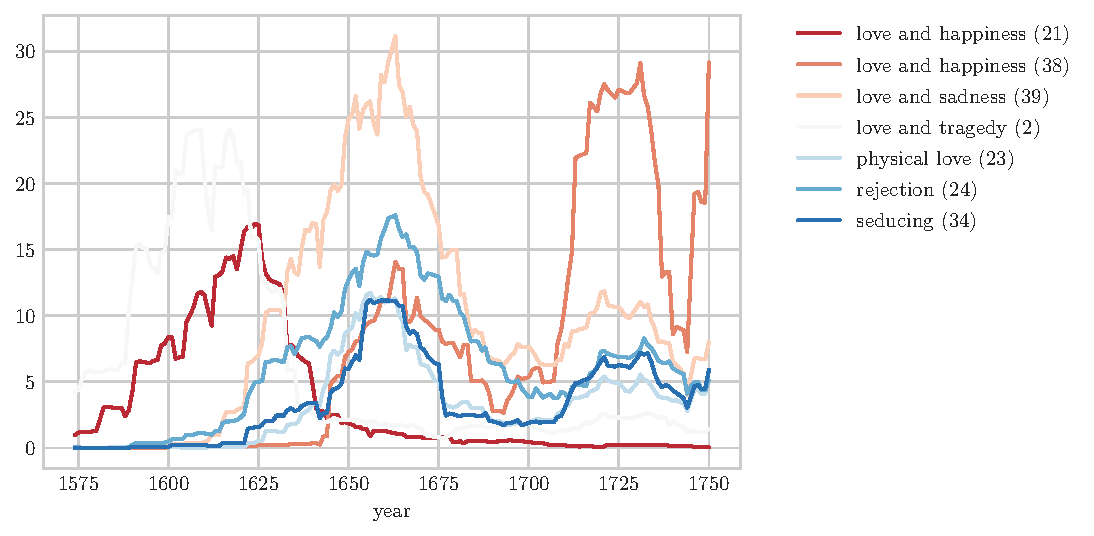
\includegraphics[scale=0.8]{love_extended}
	\caption{Love topics}
	\label{fig:love_extended}
\end{figure}

Other topics which can be related to the humanistic tradition, are \textit{bucolic songs} (47), \textit{myth and beauty} (14) and \textit{nature} (37), which I plotted in Figure~\ref{fig:bucolic}. With \enquote{bucolic}, I refer to the \enquote{pastorale} or \enquote{sheperd's song}, a popular genre in the seventeenth century. The bucolic song originates from the classics, when poets such as the Greek Theocritus and the Roman Virgil were famous bucolic poets. The use of mythological figures, such as \enquote{venus} and \enquote{phoebus} from topic 14, indicates the imitation of classical genres and topics.

\begin{figure}[hbt!]
	\centering
	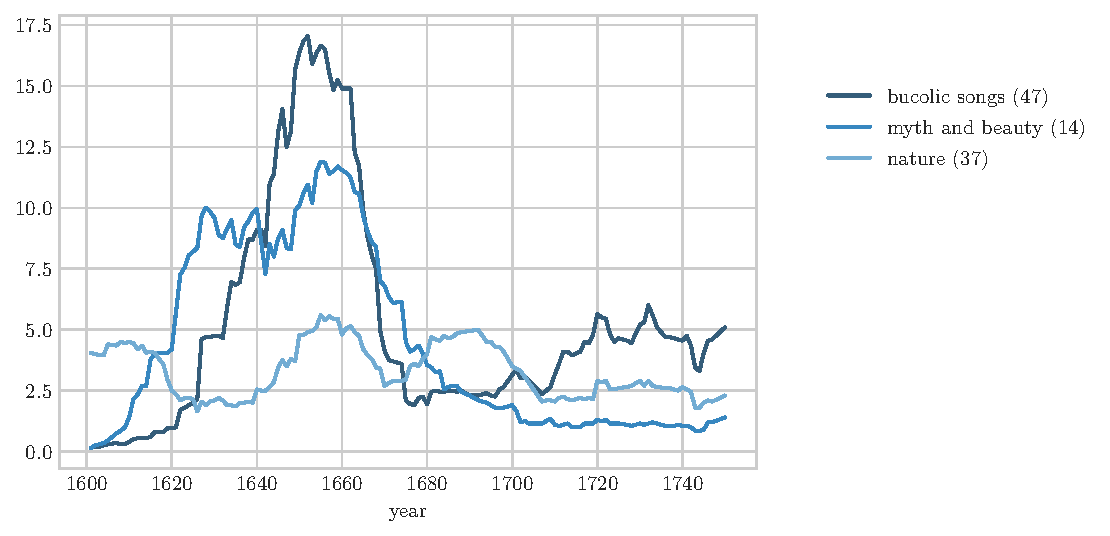
\includegraphics[scale=0.8]{bucolic}
	\caption{Renaissance topics}
	\label{fig:bucolic}
\end{figure}

As from 1660, I see a clear decline of these topics. It is important to realize, though, that the total distribution of songs in my corpus declines as well as the seventeenth century ends (but inclines again at the beginning of the eighteenth century). Still, an evident pattern can be observed in the love topic distribution in the eighteenth century. Topics on \textit{love and sadness}, \textit{love and tragedy} and \textit{rejection} are overruled by a topic on \textit{love and happiness}. According to Figure~\ref{fig:love_extended}, the Petrarcian tradition seems to move to the background, making room for a less dramatic, and more light-footed interpretation of love.

\section{Literature and politics}
Regarding the relation between literature and politics, I already mentioned the claim from contemporary research that, during political crises, literature with such crises as subject is written and read more often. If that is correct, I should see an increase of topics related to country, war and enemy, during times in which the Dutch Republic was in a precarious political situation. Although war was more of a rule than an exception in the history of the Dutch Republic, there are for sure some moments to indicate in which the crisis was peaking. First and foremost there is the Eighty Years' War, lasting from 1568 until 1648, in which the Dutch struggled for independence from the Spanish king. Although the war was interrupted for the Twelve Year's Truce, which was set from 1609 until 1621, this did not lead to a quite and carefree period in the Dutch Republic: two factions emerged as result of a theological disagreement between two professors in theology from the University of Leiden about the predestination. The debate was not limited to the religious discourse, but grew into a national conflict, concerning the question how and by whom the correct dogmas of the Reformed Church (\enquote{Gereformeerde Kerk}) should be decided.\autocite[40]{prak_gouden_2012} The conflict culminated in 1619 in the death sentence of Johan van Oldebarnevelt, the land's advocate of the Republic, simultaneously with the Synod of Dort in which the controversy around the remonstrants and counter-remonstrants was settled by sentencing counter-remonstrantism to heresy. As a result, prince Maurits managed to end the intern agitation before the Truce itself ended.\autocite[47]{prak_gouden_2012} In the end, the dispute ensured an uninterrupted uproar in the Republic for eighty years, since the Revolt continued after the Twelve Year's Truce ended in 1621. After an up and down wavy continuation of the battle, without a substantial difference in power, the Peace of Münster was finally signed by the Dutch Republic and the Spanish Crown in the winter of 1648, indicating the end of the Revolt.\autocite[53]{prak_gouden_2012} Summarized, if there is one period in which songs with nation and war as topic should be excelling, it has to be during the Dutch Revolt.

The results from the last paragraph of Chapter 7 already showed that, after adding reprints to my corpus, the topic on \textit{nation and country} is positioned at the bottom of the Top10 dominant topics. Related topics seem to be topic 7 on \textit{God and enemy} and topic 49 on \textit{God and country}, and therefore I plotted these three topics together in Figure~\ref{fig:nation}. It turns out that \textit{nation and country} starts to appear as most dominant topic of a song around 1580. Striking is the fact that the line does not start close to zero, but close to ten: the songs seem to appear almost out of nothing. In the next forty years, the number of songs per year with this topic as their dominant one, only rises. This sudden increase in popularity clearly indicates that songs with this topic were written, read and sung much more often during that time. Dominant words show that this topic is indeed on the Revolt, which is mainly illustrated by words as \enquote{prins}, \enquote{land}, \enquote{graaf}, \enquote{spaensche} and \enquote{paus}. This confirms the hypothesis that there should be an increase of topics related to country, war, and enemy, during the Eighty Years' War. In the previous chapter I already suggested that the Geusen songbooks were probably largely responsible for the sudden popularity of this topic. The line of topic 32 in Figure~\ref{fig:nation} confirms that expectation: it appears around the same time as the oldest known edition of \textit{Een nieu geuse lieden boexcken} dates from, which is the year 1577 or 1578.\autocite[75]{porteman_een_2009} Around 1640, the graph line of topic 32 shows a drastic fall, which can be explained with the end of the Dutch Revolt in 1648.

\begin{figure}[hbt!]
	\centering
	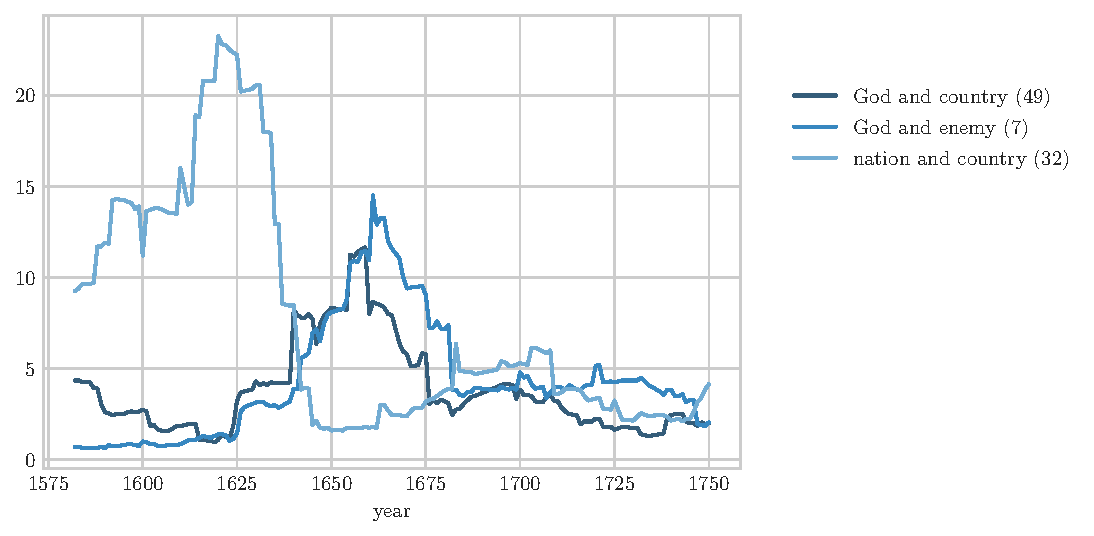
\includegraphics[scale=0.8]{nation}
	\caption{Nation, country and politic topics}
	\label{fig:nation}
\end{figure}

Remarkable is that, at the same time, two other relatable topics are rising, namely the one on \textit{God and country} (49) and \textit{God and enemy} (7). However, this does not come as much as a surprise, if you realize that the peace in the Dutch Republic only lasted until Stadtholder William II did a failed attempt to take over the city Amsterdam and therefore increase his power in 1650.\autocite[55]{prak_gouden_2012} He died a couple of months later, leaving his highly pregnant wife behind. It was the start of the First Stadtholderless period, which lasted until 1672. Again, the Dutch Republic was in turbulent waters. Although they were much more important than many a monarchy in the second half of the seventeenth century, the search for a new balance of power in Europe was accompanied by a long series of wars. Between 1652 and 1674, the Republic fought three wars with England.\autocite[57]{prak_gouden_2012} That could be an explanation for the topics on country and enemy that are still prevalent, after the end of the Revolt.

However, there are some differences between topic 32 on the one hand, and the topics 7 and 49 on the other hand. An important contrast is the major absence of religious words in topic 32. The word \enquote{god} is part of this topic, but it is the only word from the religious domain, and, moreover, it is less prevalent than words such as \enquote{prins}, \enquote{land}, \enquote{stad} and \enquote{vijand}. The topics 7 and 49, however, contain much more overlap with other religious topics, with the presence of words such as \enquote{god}, \enquote{boze}, \enquote{gods}, \enquote{handen} in topic 7, and \enquote{god}, \enquote{zijnen}, \enquote{naam}, \enquote{heren} and \enquote{hemel} in topic 49. I therefore suspect that these songs are religious songs with a strong focus on the aspect of war, peace, enemy, and the people. The song with the highest contribution of topic 49, turns out to be a psalm in the translation of Petrus Datheen (\texttt{id} =  7998), the song with the highest contribution of topic 7 is from the songbook \textit{Stichtelijcke Gesangen, behelsende: Bybelsche In-vallen. Geestelijcke Bedenckingen. Eerlijcke Vermaeckingen.} from 1661 (\texttt{id} = 155823). It is therefore also possible that the rise of these two topics has something to do with the earlier mentioned rise of reformed songbooks after 1650.

\section{Literature and diversity}
The last claim on the role of literature in early modern times I will test, is the one on diversity of both the people that were involved with literature, as well as the topics in literature. I already cited Veldhorst, who made clear that poor and rich, young and old were engaged with songs during the seventeenth century.\autocite[217]{veldhorst_pharmacy_2008} Furthermore, several studies have shown that songbooks printed especially for young readers started to appear at the beginning of the seventeenth century.\footnote{See for example \autocites{stronks_dees_2014}{grootes_het_1987}.} Their number only increased as the years passed. In the introduction of a twentieth century edition of G.A. Bredero's \textit{Groot lied-boeck}, F.H. Matter designates the publication of \textit{Den nieuwen Lust-hof} in 1602 as the beginning of a new era, in which more and more songbooks appear that are especially intended for the youth, as appears from their title or preliminary work.\autocite[18]{bredero_g._1975} A major part of the songs were on love, but not all of them. Matter asks himself why poets and printers were keen to gain the favor of the youth by producing songbooks especially for them. He does not believe that their one and only reason was the fact that youth is continuously in love and therefore yearns for love songs. Other possible explanations Matter mentions, are that youth represents a potential market since they were rather prosperous, that they are not yet seized by household worries, and that youth can be related to modern, anti-traditional and sensitive to new movements in art and literature.\autocite[19]{bredero_g._1975}

Another group that became more and more involved in literature, are women. Although male authors dominate the literary history, we know from several studies that female authors and readers were not absent during the early modern centuries. The extensive study \textit{Met en zonder lauwerkrans. Schrijvende vrouwen uit de vroegmoderne tijd 1550-1850: van Anna Bijns tot Elise van Calcar} on writing women in the early modern time shows that women were active in both the profane and religious domain, and in very different genres.\autocite{schenkeveld-van_der_dussen_met_1997} The sisters Anna and Tesselschade Roemers Visscher, Katharina Lescailje and Titia Brongersma are the most famous examples of female poets, but Schenkeveld-van der Dussen et al. determine more than seventy female writers from the seventeenth century alone. Women wrote poetry on all sorts of worldly subjects, mostly published in anthologies. Porteman and Smits-Veldt notice that, in contrast to male poets who started to publish collection bundles from the second half of the seventeenth century, this did not happen for the literary works by women.

Regarding female poets who wrote religious poetry, they put themselves completely at the service of the purpose of their texts: spiritual foundation and consolation.\autocite[840]{porteman_een_2009} Many of them were pastor's wives, and their work was in line with the tradition of the Further Reformation. From about 1670, collection bundles from female poets began to be published as well. These bundles were for the most part filled with poetry on religious subjects, and sometimes alternated with poets on worldly subjects. Authors from such mixed bundles saw their writership as subservient to the religious community they belonged to. If they discussed worldly subjects in their poetry, this happened still in a religious perspective. In some cases, the intended public of female writers were women as well. The addressates of sixteenth-century poet Vrou Gerrits' bundle are her sisters in Christ, and for Cornelia Teellinck's work, a female readership is assumed as well.\autocite[51]{schenkeveld-van_der_dussen_met_1997} Geertruida Sluiter states explicitly that she is writing to clearly formulate her faith and help fellow females with that. However, we can not assume that women were only writing for women, since there are as much examples that prove the opposite, for example the works of the eighteenth-century poet Geertruyd Gordon.\autocite[840]{porteman_een_2009} 

With the methods used in this thesis and the results obtained with it, it is hard to check whether the above claims are confirmed by quantitative research. I can see that certain love topics become more and more prevalent indeed, but topics do not give me insight in the writer of a lyric or the intended public of a song. It is possible that there are changes in the gender of characters that are subject of a lyric, but the use of a stop list ensures that personal pronouns which might suggest something on this, are excluded from the composed topics. To test the above claims, other quantitative methods should be used, for example an analysis of the preliminary works of songbooks to get insight in the intended public of a literary work.

My methods are more useful to say something about the growing diversity of topics in my corpus over time. The turnover, which I discussed previously in Chapter 3 and Chapter 6, can show me if the same topics stay the most popular over a longer period of time, or if the composition of the upper part of the ranking constantly, or during a certain time period, shifts. To compute the annual turnover of topics, I followed the steps I formulated earlier in Chapter 6. From the DataFrame I created in Chapter 7, I extracted the most dominant topic for each song. Afterwards I grouped these topics by year, and counted the number of appearances for each topic in every year. In this way, I could create an annual popularity index, containing all song topics, ranked according to their frequency of appearance in descending order. I used the following block of code:

\begin{lstlisting}
import numpy as np
import pandas as pd

top3topicsong = pd.read_csv("top3topics_allsongs.csv", sep="\t", index_col=0)
groups = top3topicsong.groupby("year")

year2index = {year: i for i, year in enumerate(sorted(top3topicsong.year.unique()))}
X = np.zeros((top3topicsong.year.unique().size, 50))
counts = groups["top1"].value_counts()
for (year, topic), count in counts.iteritems():
topic = int(topic.replace("topic ", ""))
X[year2index[year], topic] += count

turnovertop1 = np.array([x[::-1] for x in X.argsort(1)])
\end{lstlisting}

\noindent The result is a \texttt{numpy} matrix in which each array corresponds with a year, and consists a list of topics, ranked from the most dominant to the least dominant. Note that the length of the matrix is 196: the years are numbered from 0 to 195. This means that five years, from which no songs are present in my corpus, are excluded from the matrix. It concerns the years 1555, 1606, 1691, 1726, and 1729. For each position in the ranked lists, I count the number of \enquote{shifts} in the ranking that have taken place between two consecutive years. This \enquote{number of shifts} is called the turnover. Computing the turnover for all time steps in our collections yields a turnover series.

However, calculating the turnover of this ranking would not make sense, since all fifty topics appear in each ranking every year. The number of shifts would therefore always be zero, resulting in a flat graph line. Therefore I use a cutoff, to only include the upper part of the ranking in the calculation of the annual turnover. I use the following code for that (after I converted the \texttt{numpy} matrix to a \texttt{pandas} DataFrame):

\begin{lstlisting}
df_turnoverseries = pd.DataFrame(turnovertop1)
cutoff5 = df_turnoverseries[[0, 1, 2, 3, 4]].copy()
cutoff10 = df_turnoverseries[[0, 1, 2, 3, 4, 5, 6, 7, 8, 9]].copy()
\end{lstlisting}

\noindent My new DataFrame \texttt{cutoff5} contains the Top5 topics for each year, while \texttt{cutoff10} contains the Top10 topics for each year. As said before, the turnover can be defined as the number of new topics that enter a popularity-ranked list at position \textit{n} at a particular moment in time \textit{t}. Therefore I need to compare two rankings of two consecutive years and return the size of their difference. Karsdorp, Kestemont and Riddell have defined the function \texttt{turnover} as following:\autocite[134]{karsdorp_humanities_2019}

\begin{lstlisting}
def turnover(df):
df = df.apply(set, axis=1)
turnovers = {}
for year in range(df.index.min() + 1, df.index.max() + 1):
name_set, prior_name_set = df.loc[year], df.loc[year - 1]
turnovers[year] = len(name_set.difference(prior_name_set))
return pd.Series(turnovers)
\end{lstlisting}

\noindent I invoke the function with the following lines of code:

\begin{lstlisting}
turnover_topics_5 = turnover(cutoff5)
turnover_topics_10 = turnover(cutoff10)
\end{lstlisting}

\noindent The DataFrame \texttt{turnover\_topics\_5} now contains 196 rows, with each row containing a number between 0 and 5, corresponding with the number of shifts that have taken place between two consecutive years. The same applies for the DataFrame \texttt{turnover\_topics\_10}, except that each row in this DataFrame contains a number between 0 and 10. In Figure~\ref{fig:annualturnover5}, the absolute turnover of the Top5 song topics per year are plotted, while Figure~\ref{fig:annualturnover10} contains the same plot for the Top10 song topics per year.

\begin{figure}[hbt!]
	\centering
	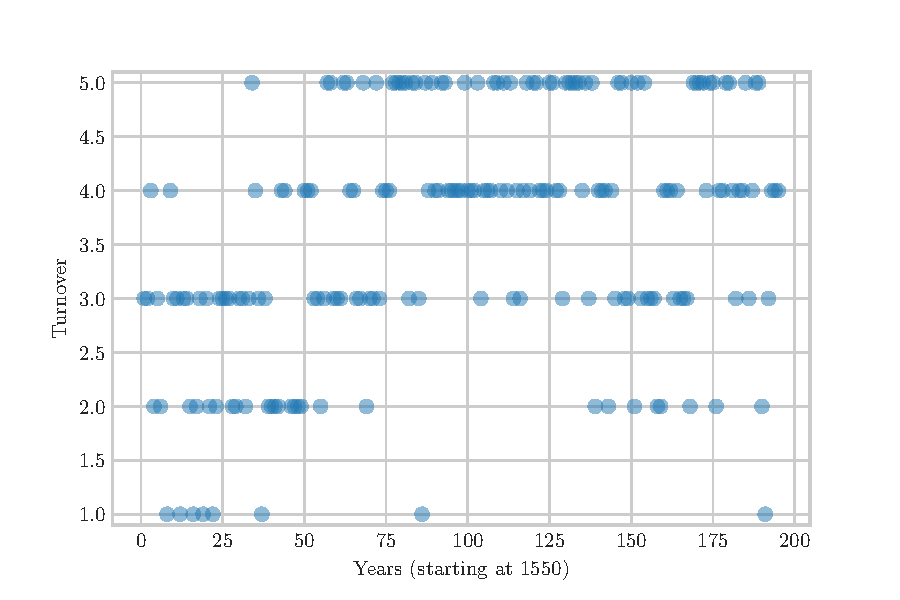
\includegraphics[scale=0.8]{annualturnover5}
	\caption{Absolute turnover of Top5 song topics (1550-1750)}
	\label{fig:annualturnover5}
\end{figure}

\begin{figure}[hbt!]
	\centering
	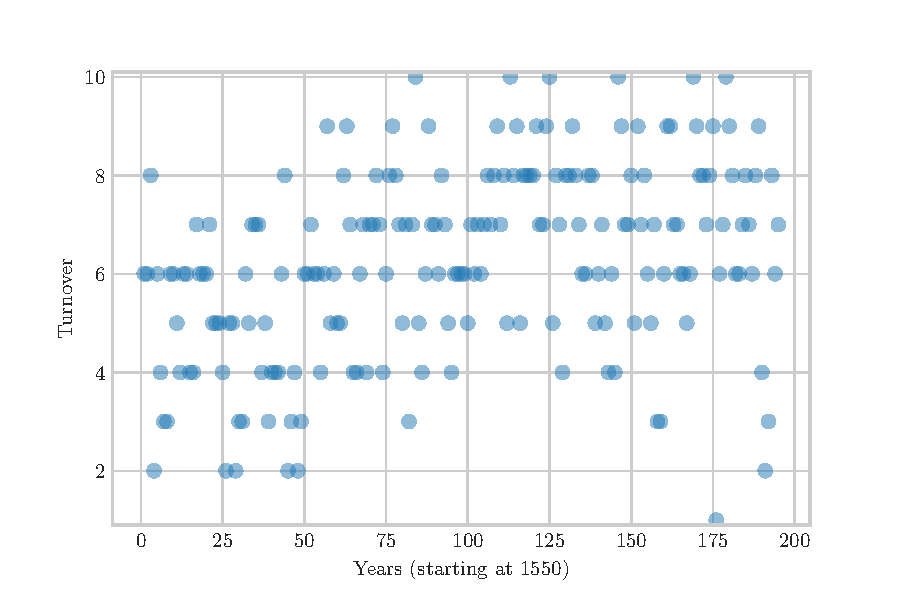
\includegraphics[scale=0.8]{annualturnover10}
	\caption{Absolute turnover of Top10 song topics (1550-1750)}
	\label{fig:annualturnover10}
\end{figure}

The reason why there are no numbers on the x-axis that can be recognized as actual years, is that earlier on, I converted the years to an index, from which five years were excluded of which I had no songs. The shortage of these years slightly distorts the image, but roughly the numbers on the x-axis can be converted to the actual years, by adding 1550 to it. According to Figure~\ref{fig:annualturnover10}, a higher turnover seems to appear from 1600. From 1625 to 1700, a turnover value below 3 does not even appear, which means that during this period, every year at least three new topics appear in the Top10. The same trend can be observed in Figure~\ref{fig:annualturnover5}. Between 1550 and 1600, the number of new topics in the Top5 is located between 1 and 4, but between 1625 and 1700, this number is in general somewhere between 3 and 5. Still, the plots in these figures are not very easy to interpret. Therefore it is helpful to use a smoothing function, which can make the visual intuitions I just made more clear. I use the \enquote{moving average} function, in \texttt{pandas} available through the method \texttt{rolling}. This function takes a couple of datapoints and returns the average of these datapoints. With the argument \texttt{window} I specify the size of the window, i.e. how many previous data points the function should take to calculate the average value. In the following code block I set the window size to 10 and create a plot afterwards:

\begin{lstlisting}
turnover_rw_10 = turnover_topics_10.rolling(10).mean()
plt.rc("text", usetex=True)
plt.rc("font", family="serif")
turnover_rw_10.plot()
\end{lstlisting}

\noindent The same I did for the DataFrame \texttt{turnover\_topics\_5}. Figures~\ref{fig:rolling5} and~\ref{fig:rolling10} show the resulting plots. When looking at Figure~\ref{fig:rolling5} in more detail, I observe a clear increase in turnover regarding the years 1550-1675. Between 1675 and 1720, the line drops, but starts to rise again after 1720. This rise only endures until 1735: by then the line drops again. In Figure~\ref{fig:rolling10}, more or less the same pattern can be observed. This means that starting around 1600, the number of topics that are in the upper part of the ranking in two consecutive years, quickly decreases. In other words: every year, more new topics make their appearance in the Top5 or Top10 of most dominant topics. This confirms the claim that a growing variation in subjects appeared during the seventeenth century.

\begin{figure}[hbt!]
	\centering
	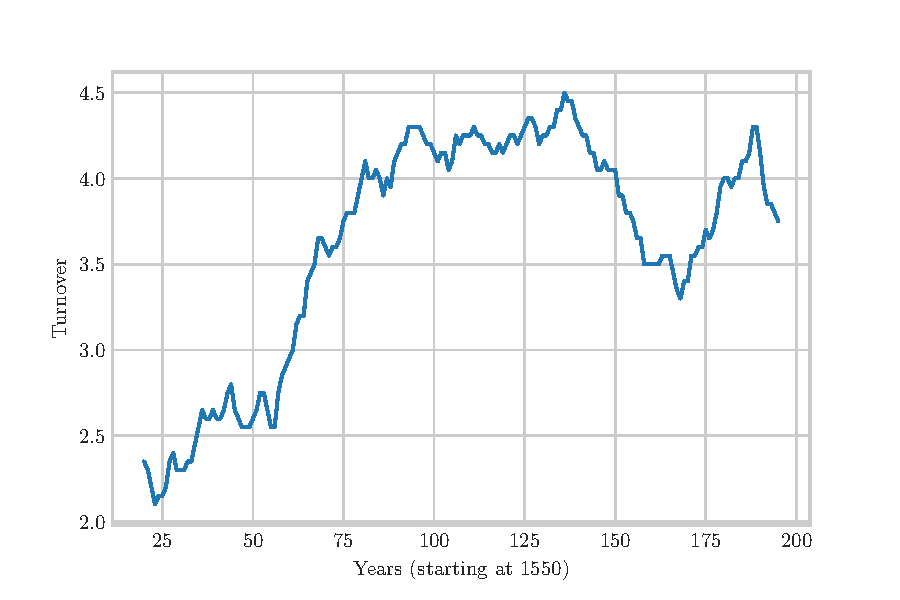
\includegraphics[scale=0.8]{rolling5}
	\caption{Moving average turnover of Top5 song topics (1550-1750, window = 20)}
	\label{fig:rolling5}
\end{figure}

\begin{figure}[hbt!]
	\centering
	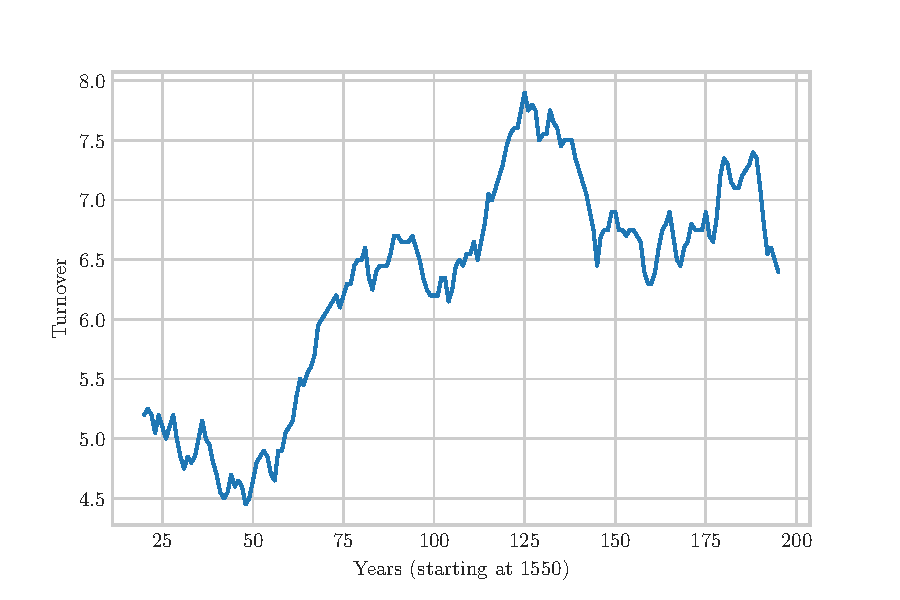
\includegraphics[scale=0.8]{rolling10}
	\caption{Moving average turnover of Top10 song topics (1550-1750, window = 20)}
	\label{fig:rolling10}
\end{figure}

In Chapter 3, I already discussed the different biases that can be at stake in a process of cultural evolution. I mentioned the study of Acerbi and Bentley, who showed a \enquote{concave} turnover profile for the turnover of recent baby names in the United States. The decreasing slope of the curve suggests a preference for relatively uncommon names, which they assign as an anti-conformity bias. The opposite was the case for early boys names, where an increasing slope suggested a preference for common names, in which Acerbi and Bentley recognized a conformity bias. In order to derive a certain bias from a turnover plot, Acerbi and Bentley use a variable top size to calculate the average turnover for each value of the top size. Plotting these two against each other, reveals whether more shifts appear in the bottom of the chart, or in the upper part of the chart. More shifts in the bottom part of the chart results in an increasing slope of the curve and therefore a conformity bias. More shifts in the upper part of the chart results in a decreasing slope of the curve and therefore an anti-conformity bias. In the turnover series that is depicted in Figure~\ref{fig:rolling5}, a fixed top size is used, namely \textit{y} = 5. To create a comparable plot as the ones Acerbi and Bentley plot, I need to calculate the average turnover for every length of the chart. I use the next block of code for that:

\begin{lstlisting}
def slicing(i):
cutoff = df_turnovertop1.iloc[:,0:i]
return cutoff

def turnover(i):
cutoff = slicing(i)
turnco = cutoff.apply(set, axis = 1)
turnovers = {}
for year in range(turnco.index.min() + 1, turnco.index.max() + 1):
name_set, prior_name_set = turnco.loc[year], turnco.loc[year - 1]
turnovers[year] = len(name_set.difference(prior_name_set))
return pd.Series(turnovers)

max_y = 51 
scores = []

for i in range(1, max_y):
avg_turnover = np.mean(turnover(i))
scores.append(avg_turnover)
\end{lstlisting}

In Figure~\ref{fig:turnoverbias51}, the result of the code above is plotted, with \texttt{max\_y} = 51. This means that for every length of the rank (starting with 1), the average turnover is calculated, ending at 50. Looking at the plot, it immediately becomes clear that this curve does not give any insight in possible biases. The reason for that is that in the ranking of song topics, a fixed number of fifty topics fill the charts. The closer the top list size comes to 50, the less topics are excluded, eventually resulting in a turnover of 0: all topics are included in the Top50, so no shifts have taken place. At first it sounds reasonable to create a plot with no negative slope, which means that the top list size should not be larger than 20, but in the end, that would not give extra insight. Since the shape of the curve in Figure~\ref{fig:turnoverbias51} is parabolic, a cutoff would always show a curve with a decreasing slope. According to Acerbi and Bentley, a decreasing slope suggests an anti-conformity bias, but in this case, it is more of a \enquote{parabolic bias}, which has nothing to do with the transmission of traits. Deriving a transmission bias from a turnover plot on early modern song topics will only make sense if the number of different topics is not equal to the maximum top list size.

\begin{figure}[hbt!]
	\centering
	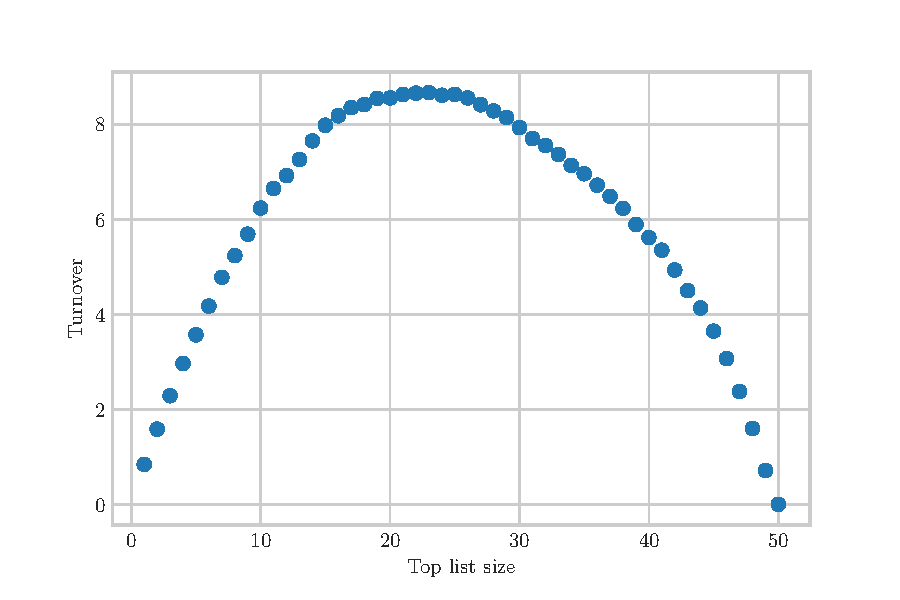
\includegraphics[scale=0.8]{turnoverbias51}
	\caption{Average turnover per top list size}
	\label{fig:turnoverbias51}
\end{figure}



\part{Conclusion}
	\chapter{Conclusion and discussion}

For years, literary researchers on the early modern period have published studies on countless well-known and less well-known early modern texts and authors, enough to fill complete libraries. These qualitative studies have shaped our idea about the Dutch Republic, her inhabitants, leaders, enemies, and in particular, her literature. To some extent, it is understandable that these researchers are a bit wary of new, digital methods to investigate cultural products from a larger distance. Zooming out means that many details become invisible: details which, with close reading, would have given us essential information about a text, its writer, publisher, reader, or the context in which it was created. However, in words of Underwood, \enquote{[a] single pair of eyes at ground level can't grasp the curve of the horizon}.\autocite[x]{underwood_distant_2019} If we take our distance and get up in the sky, we will see things, patterns, we were never able to see before. This does not mean that we should forget the observations we did earlier, when we were still on our knees, studying a text through a magnifying glass. The golden mean shall always be a combination of both: a confrontation of the one method with the other, to see how both perspectives are related to each other and how they can complement each other.

That is what I have tried to do in this thesis. In researching a corpus of Dutch early modern songs from a larger distance, I have not only added a study to the very long list of studies on Dutch early modern song culture, but most of all, I have expanded the very short list of \textit{quantitative} studies on the Dutch early modern song. The answers I have found on the twofold question I asked in the first chapter of this thesis, are probably not the most surprising. However, the application of digital methods to a corpus of 43,772 Dutch songs was a rather unexplored area. With the results obtained in this research and the interpretation of these results, I have combined the two perspectives mentioned above (close and distant reading), and evaluated if and how the outcome of qualitative research on the one hand and quantitative research on the other hand can be related to each other. I do believe that the combination of these two methods and the confrontation with each other can help the early modern literary studies reach a new level.

The first of the two questions I asked was which topics the most dominant were in early modern Dutch songs. In answering this question, the preliminary steps I had to take before I was actually able to let the computer compose topics, took the most time. In the previous months, during my internship at the Meertens Institute, I had gained enough knowledge on skills such as parsing XML-files, that this was no longer a problem. However, the enormous variation in spelling of these songs turned out to be a big bump. Working with a corpus containing texts from a period of two hundred years in which no normalized spelling was set, was in this case a very complicating fact. I use the words \enquote{in this case}, because I realize that there are also situations in which this variation is no problem, or even desirable, for example to investigate how fast or slow the spelling of words change over time. In the context of this thesis, however, it was very important that all texts were normalized to the same spelling. For topic modeling it is necessary that a word is spelled exactly the same way through time, otherwise the computer will build different topics for situations in which one topic would be sufficient.

To normalize historical spelling, there are several methods available for the English language, but regarding the Dutch language, options were limited. The very straightforward INL-tool I used had been helpful in a sentiment analysis of early modern songs, but in this study, the tool worked too sloppy and the results were therefore too unreliable. The VARD2-tool I tested had much more potential, especially because the tool gave an output file in which all made changes were reported. The fact that the training set of the tool was build from seventeenth century translations of the Bible, had both advantages and disadvantages. I already knew that a major part of my song corpus consisted of religious songs, so there would be a lot of overlapping words between the Bible and my corpus. The dating of the training set in the seventeenth century, had the disadvantage that older words (from the fifteenth or sixteenth century) were not included in the set. \enquote{Old} words in songs, such as \enquote{dijn}, were therefore not normalized by the tool. Still, I considered the VARD-normalized version of the corpus as the best version, and therefore continued my analysis with that one.

Of all the digital methods to research literary texts computationally that have arisen in the last decades, I have chosen a rather controversial one in this thesis. Topic modeling is widely discussed, not only because it is based on probabilities and the mathematical idea therefore seems a mystery to many users, but also because we know that the tool needs improvement and is not already at its best at the moment. Changing some settings, for example the number of topics or the number of iterations, can highly influence the output. I therefore have had rerun the tool several times, searching for the best settings. In this study, as well as for all studies in which computational methods are used, it is of great importance to critically evaluate the methods used. Although I have done that to some extent, I realize that there are still aspects that could have been evaluated more. Another point where human intervention may have influenced the results negatively, is the assigning of a certain subject to topics. I have done this assigning by looking at the word cloud of a topic, in which more dominant words were depicted larger than less dominant words. I have tried to include this difference in word dominance in my consideration which subject would describe the topic at best, but still it is possible that, if someone else would have done the topic assigning, different subjects would be given to the topics, simply because a human being can never be as objective as a computer -- which, actually, is why a computer is never 100\% objective as well, since I am (or somebody else is) the one building the tool.

This finally brings me to the answer on the first part of the twofold research question, what the most dominant topics in my corpus were. As said before, the answer did not come as a surprise. Based on the genre distribution in my corpus, I already expected the religious topics to be by far the most dominant. However, what the genre distribution of the Dutch Song Database does not show, are the subcategories within a genre. Furthermore, a genre does not say anything about the topic of songs within that genre. Those insights are obtained by building topics from the corpus. Apart from all criticism, it is admirable that the topic modeling tool was able to distinguish between songs on, for example, \textit{love and tragedy}, and songs on \textit{rejection}. Another remarkable observation was the dominance of songs with \textit{nation and country} as their most dominant topic, especially after adding the reprints and songs from other songbooks to the corpus. It is necessary to discuss the method I used in choosing the most dominant topic for each song. The output of a topic modeling tool is always a distribution over the number of topics you let the tool made. In the context of this study, it meant that theoretically, fifty topics were present in each song, and the sum of their contributions was always one. However, for each song there was of course a vast majority of topics that was not present, and their contribution was very close to (but never) zero. At the same time there was always one topic that stood out as most dominant. In a lot of cases, the contribution of that topic was quite high (0.6 or higher), but there were also songs in which the topic with the highest contribution still had a very low contribution, in the worst cases even below 0.2. To be pragmatic I have limited my choice to the most dominant topic for each song (regardless how small or large the contribution of that topic), but I realize that this undoubtedly has biased my results.

In answering the second part of the research question -- investigating topical fluctuations in a diachronic corpus -- the curve of the horizon Underwood spoke about, came into view. I zoomed out in order to see which patterns became visible by observing topics over a longer period of time. What I learned is that, speaking in general, every topic peaked at one particular moment. It means that most of the topics are not equally dominant at all times, but appear, peak and disappear at a certain moment. To what extent is this relatable to spelling and word choice? Is it possible that songs from the same period stick together anyway, because they look like each other regarding their words, and the way these words are spelled? This is exactly what I have tried to eliminate by using a spelling normalization tool, but since this tool has its limits as well, it is possible that I only partly succeeded in this. Still, intuitively I can not imagine that this is the only reason for the sharp peak in every topical plot. Above all, it suggests how certain topics appear and disappear over time, making room for other topics which are often very similar, but still at an important point different, otherwise these songs would have had the same dominant topic.

In my thesis, I have related topical fluctuations to cultural-historical changes. It turned out that several topics can be related to certain events in the Dutch Republic, for example the rise of Petrarchism, the Eighty Years' War and the heydays of the Further Reformation. A question that rises from these results is: are songs a predictor or follower of trends? Do songs arise as the result of a certain trend, or are they boosting a certain trend? From previous, qualitative studies, we know that both options were common in the early modern times. The number of songs of the Further Reformation, for example, grew because Calvinists published their own songbooks in high circulation. In these songs, subjects were described which were already discussed and preached about in churches. The Wilhelmus, however, is an example of a song that functioned more as a booster of a trend, namely the revolt against the Spanish king. In the end, I think that the current results are too roughly meshed to say something wise about this matter. Other methods will undoubtedly be more suitable to answer this question.

More than exploring the relationship between topical fluctuations in my results on the one hand and cultural-historical changes in the Dutch Republic on the other hand, I mainly explored how my results, obtained with quantitative research, can be related to the \textit{status quaestionis} in qualitative research on Dutch early modern literature. Which roles are assigned to literature, concerning the early modern centuries? I distinguished four of them and explored whether my obtained results could validate these four theses. Regarding the relationship between literature and ideology, I illustrated with songs from the Further Reformation how a certain ideology is carried out in song lyrics. The relationship between literature and poetics of which we know, thanks to numerous qualitative studies on humanism, the classical tradition, the Renaissance tradition, and Petrarchism, was confirmed by the quantitative results regarding love topics in my corpus. Concerning the third thesis on early modern literature -- literature and politics are closely related in times of political crises -- this was confirmed mainly by the enormous number of songs with \textit{nation and country} as their most dominant topic, published during the Revolt. The last claim on the role of literature in the early modern times -- diversity in both involved people and topics -- was more complicated to test. With the used method, it is not possible to distill an intended public from a text. I already stated that other methods would be more fruitful to test this thesis. The diversity in topics I have investigated in calculating the turnover.

In calculating the turnover of topics, I came close to the theoretical field I wanted to explore in this thesis: cultural evolution. Hearing and reading about it in the months before I started to write my thesis, I had become curious about \enquote{how Darwinian theory can explain human culture and synthesize the social sciences}, to say it with Mesoudi.\autocite{mesoudi_cultural_2011} I wanted to investigate if and how cultural evolution could be applied to early modern songs. But when does a study become a study on cultural evolution? It is more than offering a diachronic perspective. Cultural evolution links certain changes in texts, or any cultural product, to cultural and historical circumstances, and human behavior. I did the \enquote{Darwin check} to see if the three preconditions of biological evolution -- variation, competition and inheritance -- could be applied to culture, and more specific, to a corpus of Dutch early modern songs. The songs survived the test, and I explored how I would be able to say something about the transmission bias that might have been at stake in human behavior when inheriting song topics. In the end, I did not gain the unambiguous result I was hoping for. I faced the limitations of either my corpus, my skills and knowledge, or the available methods.

I am almost tempted to say that culture -- and in this case, a complex corpus of songs, uneven distributed over time, and with loads of spelling variation -- is too complex for simple evolutionary models. But then Mesoudi refutes:

\begin{quote}
	It is not being argued that human culture really can be described entirely in terms of just a handful of simple variables and processes. Rather, the reduction involved is methodological: faced with an enormously complex phenomenon such as culture, the most productive approach to understanding that phenomenon is to divide it up in small pieces and try to explain them in a piecemeal style. (...) Only simple models can yield quantitative, testable predictions that can be shown to be either statistically supported or not; and if not, we simply build and test an alternative model.\autocite[131]{mesoudi_cultural_2011}
\end{quote}

\noindent Against another objection, namely that cultural phenomena are too unique and particular to be compared with each other in the way cultural evolutionists suggest, Mesoudi argues with stating that

\begin{quote}
	the aim is not to \textit{replace} the study of specific historical events or societies with general microevolutionary processes. On the contrary, without details of specific societies or time periods, there is no data with which to test the validity of the general evolutionary processes. Nor is it to deny that there are important differences between societies and time periods. Of course there are. But there are also similarities, and identifying these similarities, and explaining them with simple principles (...) surely \textit{adds} to the study of specific cases rather than detracts from them.\autocite[132]{mesoudi_cultural_2011}
\end{quote}

\noindent It is quite funny to recognize the same rhetoric as used by digital humanities scholars such as Underwood and Piper, in defending their computational methods, just as I did in the beginning of this chapter, as well as in Chapter 2. I might not have understood yet the width and depth of cultural evolution by writing this one thesis, what I do know is this: to investigate whether we can indicate cultural evolution in a corpus of Dutch early modern songs, quantitative research of these songs is necessary. But, at the same time, in order to understand the observed patterns achieved with computational methods, we need the results obtained with qualitatively researching early modern literature as well.

Using computational methods on large digital corpora, is like zooming out on Google Earth: you do not see the streets, the squares and the roundabouts anymore. Instead, you start to see cities, borders, huge woods, long rivers, mountains, deserts, oceans, and, eventually, the shape of the earth. It changes your whole perspective on the city you reside in, the country you are inhabitant of, and the continent on which you live. But to plan your route to visit a concert of Famke Louise on a pop stage you have not been before, you still use Google Maps. And that is okay. Because the one does not have to replace the other.




\backmatter
% bibliography, glossary and index would go here.
\printbibliography[heading=bibintoc]
\chapter{Stop list original corpus}

\begin{minipage}[t]{0.25\textwidth}
	en\\
	die\\
	in\\
	de\\
	van\\
	dat\\
	u\\
	een\\
	met\\
	't\\
	is\\
	mijn\\
	niet\\
	ick\\
	te\\
	den\\
	hy\\
	my\\
	het\\
	al\\
	op\\
	ons\\
	als\\
	ghy\\
	’\\
	zijn\\
	tot\\
	daer\\
	haer\\
	voor\\
	om\\
	soo\\
	sijn\\
	hem
\end{minipage}
\begin{minipage}[t]{0.25\textwidth}
	door\\
	sy\\
	sal\\
	maer\\
	ik\\
	dan\\
	heeft\\
	t\\
	gy\\
	nu\\
	wat\\
	o\\
	wel\\
	hier\\
	want\\
	uw\\
	aen\\
	wy\\
	wilt\\
	dit\\
	noch\\
	by\\
	hoe\\
	of\\
	geen\\
	der\\
	myn\\
	na\\
	was\\
		moet\\
	uyt\\
	v\\
	men\\
	oock\\
\end{minipage}
\begin{minipage}[t]{0.25\textwidth}
	des\\
	‘\\
	laet\\
	seer\\
	alle\\
	doet\\
	wil\\
	veel\\
	doen\\
	zy\\
	so\\
	ende\\
	waer\\
	doch\\
	kan\\
	eer\\
	end\\
	groot\\
	siet\\
	meer\\
	haar\\
	daar\\
	schoon\\
	dus\\
	komt\\
	hebt\\
	gaen\\
	zijt\\
	vol\\
	eens\\
	zyn\\
	maar\\
	wie\\
	sonder
\end{minipage}
\begin{minipage}[t]{0.25\textwidth}
	'k\\
	goet
	ten\\
	's\\
	d\\
	ter\\
	soet\\
	dees\\
	aan\\
	ben\\
	gaet\\
	uwen\\
	wesen\\
	naer\\
	syn\\
	heb\\
	zal\\
	nae\\
	uwe\\
	zoo\\
	staet\\
	gheen\\
	int\\
	toe\\
	vry\\
	hebben\\
	dien\\
	weer\\
	lust\\
	sult\\
	mach\\
	geeft\\
	dese\\
\end{minipage}
\chapter{Stop list INL-normalized corpus}

\begin{minipage}[t]{0.25\textwidth}
	en\\
	ik\\
	die\\
	de\\
	in\\
	u\\
	van\\
	dat\\
	zijn\\
	een\\
	met\\
	al\\
	't\\
	is\\
	te\\
	mijn\\
	niet\\
	den\\
	ons\\
	het\\
	op\\
	als\\
	haar\\
	hebben\\
	’\\
	hei\\
	tot\\
	gij\\
	voor\\
	clitic\\
	om\\
	zullen\\
	hem
\end{minipage}
\begin{minipage}[t]{0.25\textwidth}
	door\\
	deze\\
	daar\\
	doen\\
	zo\\
	na\\
	dan\\
	nu\\
	t\\
	aan\\
	wat\\
	zij\\
	o\\
	wel\\
	hier\\
	want\\
	uw\\
	gaan\\
	uit\\
	god\\
	of\\
	maer\\
	noch\\
	geen\\
	hoe\\
	gei\\
	ook\\
	der\\
	hy\\
	zeggen\\
	wi\\
	was\\
	moet
\end{minipage}
\begin{minipage}[t]{0.25\textwidth}
	v\\
	maar\\
	daer\\
	bij\\
	ick\\
	staan\\
	men\\
	des\\
	‘\\
	eend\\
	wild\\
	soo\\
	zoet\\
	eer\\
	groot\\
	komen\\
	wil\\
	veel\\
	kan\\
	sieren\\
	WAAR\\
	laat\\
	ghy\\
	mogen\\
	doch\\
	sy\\
	schoon\\
	geest\\
	wie\\
	meer\\
	waard\\
	maken\\
	dus\\
\end{minipage}
\begin{minipage}[t]{0.25\textwidth}
	sullen\\
	hoog\\
	vol\\
	eens\\
	goed\\
	wilt\\
	kwaad\\
	wees\\
	lief\\
	ten\\
	d\\
	zieden\\
	worden\\
	spreken\\
	min\\
	lang\\
	geven\\
	ben\\
	gy\\
	heb\\
	vrij\\
	laet\\
	sijn\\
	zelf\\
	zoo\\
	blijven\\
	toe\\
	gheen\\
	recht\\
	brengen\\
	alleen\\
\end{minipage}
\chapter{Stop list VARD-normalized corpus}

\begin{minipage}[t]{0.25\textwidth}
	en\\
	het\\
	in\\
	de\\
	die\\
	van\\
	dat\\
	ik\\
	u\\
	mijn\\
	zijn\\
	een\\
	met\\
	is\\
	gij\\
	te\\
	niet\\
	den\\
	hij\\
	mij\\
	zo\\
	al\\
	op\\
	als\\
	daar\\
	ons\\
	haar\\
	zij\\
	tot\\
	zal\\
	voor\\
	maar
\end{minipage}
\begin{minipage}[t]{0.25\textwidth}
	om\\
	hem\\
	door\\
	aan\\
	des\\
	o\\
	dan\\
	heeft\\
	’\\
	nu\\
	wat\\
	wel\\
	na\\
	hier\\
	want\\
	wij\\
	heer\\
	wilt\\
	dit\\
	ook\\
	uit\\
	noch\\
	bij\\
	der\\
	of\\
	laat\\
	hoe\\
	geen\\
	men\\
	was\\
	moet\\
	v\\
\end{minipage}
\begin{minipage}[t]{0.25\textwidth}
	uw\\
	zeer\\
	WAAR\\
	‘\\
	alle\\
	doet\\
	wil\\
	ziet\\
	uwe\\
	veel\\
	doen\\
	goed\\
	kan\\
	komt\\
	ende\\
	doch\\
	gaan\\
	zijt\\
	eer\\
	end\\
	groot\\
	dood\\
	meer\\
	zonder\\
	schoon\\
	gaat\\
	wezen\\
	dus\\
	zoet\\
	hebt\\
	vol\\
	naar\\
\end{minipage}
\begin{minipage}[t]{0.25\textwidth}
	eens\\
	wie\\
	mag\\
	'k\\
	staat\\
	ten\\
	geeft\\
	ter\\
	werd\\
	gelijk\\
	ben\\
	uwen\\
	syn\\
	heb\\
	maakt\\
	wordt\\
	deze\\
	zoo\\
	zult\\
	vrij\\
	weer\\
	gheen\\
	toe\\
	altijd\\
	hebben\\
	nooit\\
	staan\\
	dag\\
	dien\\
	dezen\\
	ze\\
	onze\\ 
\end{minipage}
\chapter{Topics original corpus}

\begin{longtable}{p{.10\textwidth} | p{.90\textwidth}}
	\toprule
	Topic & Words \\       
	\midrule                                                   
	0     & zo uit zich ook ziet waar laat naar zelf nooit                       \\
	1     & lof maria hemels godt moeder godts boven reyn bruydegom schoone      \\
	2     & ook god heer kerk godes goods volk werd deur christus                \\
	3     & ach hert lief min ziel pijn leven och hart smert                     \\
	4     & heer godt heere vader lof onse naem herten geest onsen               \\
	5     & hun godt leeven gaat vrolyk laat quaat waar geeven weesen            \\
	6     & ic lief es ooc moeder vader god ruyter man miin                      \\
	7     & godt kindt stal kindeken nieuwe moeder kint iaer geboren mensch      \\
	8     & hart wiens gelijk sich ook er word waar n't wijl                     \\
	9     & god laat uit leeven heer naa goed gods waar hert                     \\
	10    & prins jn jck graef paus soldaten schepen stadt onse spaensche        \\
	11    & heer godt se hen wt sullen doer ouer dies n't                        \\
	12    & herder vee groene harder coridon herders schaepjes herderin soete ey \\
	13    & man neen weet mee ander sou staen gelt maeckt huys                   \\
	14    & quam sprack sagh riep liet doe nam gaf gingh sey                     \\
	15    & hemels heer god godes sint hart goods maeght lof groote              \\
	16    & hij sij mij ghij gij wij dij bij sall vive                           \\
	17    & liefde liefd hert iesu ziel lief soete iesus min herte               \\
	18    & nog ook 'er jk zo sprak lief dog er ziet                             \\
	19    & heer jesus ook iesus nogh seydt godt vader alleluja christus         \\
	20    & ich das mein vnnd mir je vous ein le la                              \\
	21    & godt leven ziel godts heer goedt eeuwigh mensch vreught tijdt        \\
	22    & godt gods god mensch quaet wet hert wert recht menschen              \\
	23    & doodt godt sonden heer leven christus mensch bloedt lijden ziel      \\
	24    & leuen christus wt nv gods heere woort god doot godt                  \\
	25    & heer dijn godt dy god heere hun wt du dies                           \\
	26    & leven ghelijck oft gheven ooghen gheeft teghen gheest tijdt boven    \\
	27    & och doot lijden heere werelt godt noot comt verdriet herte           \\
	28    & god heer sich hand sijne hert lof goed vreughd dood                  \\
	29    & lief liefde hert adieu liefste troost reyn ic princesse mocht        \\
	30    & ziel hert heer god nog geest ook gods laat hemel                     \\
	31    & la fa bruydt vrolijck bruydegom twee man bruyt paer vreught          \\
	32    & soete min venus minne ach hemel licht schoone wiens glans            \\
	33    & godt volck godts hulp landt macht hooft tegen vyanden strijden       \\
	34    & dy yn soe uwz mey jon fen god az heer                                \\
	35    & godt hert sich godts quaedt loff wordt vw zich ziel                  \\
	36    & sprack waren godt quam gods eenen quamen heeren wt hadden            \\
	37    & sprack godt man heere quam abraham vader israel water huys           \\
	38    & mey vruchten groen groene lof winter boomen vrucht onder schoone     \\
	39    & leven heer geven god sullen gelijck komen oogen heere dagen          \\
	40    & godt hert oft liefde leven vreught godts heer heel n't               \\
	41    & vreucht comt liefd vvant deucht deur venus n't vvilt reyn            \\
	42    & gods godt christus heeren woort sullen godts desen heer hoort        \\
	43    & wijn sa drincken wyn bier boer drinckt eenen bacchus nat             \\
	44    & heer hun uit ook godt god volk heeren naar heere                     \\
	45    & ha n't waar laat gaat ho gaan va dies staat                          \\
	46    & zee schip baren varen mee ree winden schipper voort landt            \\
	47    & mit dyn god du dy ghoed zo dynen unde elck                           \\
	48    & jou je jy nou kom ja meysje ey hey och                               \\
	49    & min zo laat liefde hert nog zoet ach zoete ziel     \\
	\bottomrule      
\end{longtable}
              

\chapter{Topics INL-normalized corpus}

\begin{longtable}{p{.10\textwidth} | p{.90\textwidth}}
	\toprule
	Topic & Words \\       
	\midrule
	0     & hun leven gods vreugde eeuwig godt heemels heemel vrome dood      \\
	1     & du end dijn heer deinen huur fijn myn dyne zek                    \\
	2     & er nog jk zy dog zeer vader trouw kind adieu                      \\
	3     & heer iesus jesus christus petrus godt vinden weer zegge twee      \\
	4     & mens leven lust rust zek hert ziel vreugde alles gemoed           \\
	5     & vals mens tong boos haat elk schijn snood lust waarheid           \\
	6     & wijn drinken sa bier glas boer lustig geld bacchus wy             \\
	7     & godt volk israel heere coninck man heeren ginck david abraham     \\
	8     & heer hun volk godt heeren heil woord na?m zek hen                 \\
	9     & leven wereld godt mens tijd eeuwig sterven doden dood zonde       \\
	10    & schoonheid haer deugd lof scholen glans goud siet wit leven       \\
	11    & jij er kom nauw ja och mede meysje weer zien                      \\
	12    & ich das mein vnnd mir ein mich jn nitt zei                        \\
	13    & kerk geloof gods eerst nieuw christus godes zeer eigen heer       \\
	14    & stad waren moeten prins wy graef enten binnen menig laten         \\
	15    & zek zee hand heen water volk bloed hemel weer af                  \\
	16    & gods enten zondaar leven heere elk heeren ghelijck fijn liefde    \\
	17    & godt hert zek godts woord af waer kracht ramp leven               \\
	18    & hij ende ic ghij vader wij alzo och willen moeder                 \\
	19    & end heer godt hen zien volk n't kracht myn dies                   \\
	20    & groen herder vee harder ach waer coridon schaepjes herderin onder \\
	21    & christus gods wart leven enten ende heere dood wereld mens        \\
	22    & hert hun n't leven godt oft naer myn heel liefde                  \\
	23    & godt ziel godts vreugde vinden heer haren boven leven troost      \\
	24    & ach hert leven smart hart pijn ziel droef sterven trouw           \\
	25    & nog myn leven zeer liefde zoete dog zy nooit er                   \\
	26    & liefde enten hart deur troost vreugde ic reen hert zwaar          \\
	27    & vreugde zingen vrolijk blij zang spelen wy springen verheugd lof  \\
	28    & dijn end du heer godt dijnen dies dij alleluia godes              \\
	29    & godt maria godts lof moeder hemels boven vreugde klaar zondaar    \\
	30    & heer godt lof leven vader loven prijs hemel wy boven              \\
	31    & le vous la qui kwee mon les vive ma dobbe                         \\
	32    & zee schip mede weer varen voort land prins wy landt               \\
	33    & godt godts leven gods heer heeren werk hart altijd deugd          \\
	34    & hemels godes heer sint haer leven deugd ziel goods maeght         \\
	35    & la fa hu bom lier ta mi tiere tieren sol                          \\
	36    & du yn uwz dy fen gunnen mei az mof heer                           \\
	37    & mond venus leven kusje ach ziel brand kussen lust hart            \\
	38    & sou ander tijd weet man neen denken waer weer haast               \\
	39    & ziel zich nog gods leven hert heer zeer eeuwig nooit              \\
	40    & bloed doden dood lijden kruis leven christus godt zonde vader     \\
	41    & kind godt nieuw mens stal geboren iaer klein kinnetje moeder      \\
	42    & heer ziel hert zonde leven mijne heere troost bidden och          \\
	43    & vreugde man trouw leven vrede twee vrouw wens liefde bruydt       \\
	44    & ha venus deur goden daphne cupido mars kleur ho diana             \\
	45    & liefde hert ziel lieven hart beminnen vreugde liefd leven zin     \\
	46    & licht nacht dag ogen son slaap zon gezicht duister stralen        \\
	47    & heer godt heere hun fijn noot hart vijand enten helpen            \\
	48    & vijand strijd tegen macht geweld strijden kracht sterk godt hulp  \\
	49    & groen mey vruchten tijd vrucht groeien bloeien kruid veld winter\\
	\bottomrule
\end{longtable}
\chapter{Topics VARD2-normalized corpus}

\begin{longtable}{p{.10\textwidth} | p{.90\textwidth}}
	\toprule
	Topic & Words \\       
	\midrule                                                             
	0     & god vader geest lof leven herten onzen woord zonden naam           \\
	1     & maria moeder gods lof god hemels maagd vreugd klaar rein           \\
	2     & lief adieu liefste liefde hert troost mocht och herte minnen       \\
	3     & kwam zag sprak ging riep doe liet nam gaf stond                    \\
	4     & god oft hert vreugd gods leven heel mijnen haren liefde            \\
	5     & kind geboren god stal kindeken moeder mens nieuwe bethlehem maria  \\
	6     & dijn dij god du hun wt mit fijn dijnen recht                       \\
	7     & god volk bloed hand vijand tegen land geweld straf kwaad           \\
	8     & god hen zullen allen wt doer gants dies geprezen werden            \\
	9     & god wt leun gods nv woord christus genen si wereld                 \\
	10    & och lijden ach hert pijn verdriet ziel druk tranen droefheid       \\
	11    & mee 'er twee ieder deur mof geld klok net je                       \\
	12    & vreugd man bruid twee bruidegom geluk paar bruyt deugd trouw       \\
	13    & gods oft elk god woord heren geest enen rein leven                 \\
	14    & venus licht schoonheid gezicht glans zon goden ogen schone stralen \\
	15    & god sprak kwam zijnen enen gods volk waren ginck man               \\
	16    & kwaad elk zich recht licht waarheid mens eigen schijn haat         \\
	17    & vrolijk hemels hemel vreugd boven zon eeuwig ziel hert oog         \\
	18    & god gods mens leven woord geest godes hert recht heren             \\
	19    & leven zullen geven komen tijd maken dagen laten niemand moeten     \\
	20    & la ha fa hu bom alleluia liere vive tiere es                       \\
	21    & liefde vreugd deur rein denkt tis liefd wt nieuwe tijd             \\
	22    & kerk gods geloof godes christus deur christen werk zou iae         \\
	23    & zoete mond lieve ei ach lipjes kusjes kussen lust vreugd           \\
	24    & neen weet lang weg ander sou ei tijd man kind                      \\
	25    & zee schip land wind mee baren varen voort ree reis                 \\
	26    & geld enen man hun boer oft vrouw huis sou boeren                   \\
	27    & lust mens werelds rust ziel schat geld goud wereld zich            \\
	28    & god word geest nog ziel jezus gods leven hert naa                  \\
	29    & wijn drinken sa vrolijk drinkt lustig bier vreugd bacchus zingen   \\
	30    & nog dog lief jk 'er ag zoete kind trouw zou                        \\
	31    & gods christus god woord zullen hoort moeten heren och vrienden     \\
	32    & prins land stad vijand graaf god waren jn held kwamen              \\
	33    & zich god hert vw ren er zijns gods zelfs dies                      \\
	34    & jou je jij meisje ja kom lieve och meid ien                        \\
	35    & hun god zich hart hen leven gods volk zijne heil                   \\
	36    & ziel mijne god mijnen woord hert ziele hand ogen recht             \\
	37    & mei vruchten groen groene vrucht schone bomen winter boom land     \\
	38    & min hart liefde nog hert ziel leven vreugd ach ogen                \\
	39    & ach min lief hert liefde ziel minne pijn hart leven                \\
	40    & sprak christus jesus jezus zeid kwam petrus zeide joden nog        \\
	41    & das mein vnnd mir ein mik jn nitt zei mit                          \\
	42    & zonden kruis bloed jezus lijden jesu vader wonden god jesus        \\
	43    & le vous je la pour mon les qui ne boire                            \\
	44    & god hemels godes sint hart gods maagd ziel lof deughden            \\
	45    & dij yn soe uwz jon fen mei god nat amor                            \\
	46    & wereld god leven tijd eeuwig kwaad sterven werelds zonden mens     \\
	47    & vee herder groene zoete veld harder herders schaepjes coridon zon  \\
	48    & liefde hert liefd ziel herte ziele lief alleen zoete iesu          \\
	49    & god lof zijnen volk naam heren zijne hoog hemel looft   \\
	\bottomrule          
\end{longtable}
\end{document}